\documentclass[edeposit,fullpage,12pt]{uiucthesis2009}
% Use draftthesis for notes and date markings on every page.  Useful when you
%   have multiple copies floating around.
% Use offcenter for the extra .5 inch on the left side. Needed with fullpage and fancy.
% Use mixcasechap for compatibility with hyperref package, which does NOT like all caps default
% Use edeposit for the adviser/committee on the title page.
% Use tocnosub to suppress subsection and lower entries in the TOC.
% PhD candidates use "proquest" for the proquest abstract.

\makeatletter

\usepackage{setspace}
%\usepackage{epsfig}  % for figures
\usepackage{graphicx}  % another package that works for figures
\usepackage{multirow}
\usepackage{placeins}
\usepackage{caption}  % allows center figures caption
\usepackage{booktabs} % nice rules (thick lines) for tables
\usepackage{array}
\usepackage{tabularx}
\usepackage[table]{xcolor}
\newcolumntype{b}{>{\hsize=1.0\hsize}X}
\newcolumntype{s}{>{\hsize=.5\hsize}X}
\newcolumntype{m}{>{\hsize=.75\hsize}X}
\newcolumntype{x}{>{\hsize=.25\hsize}X}
\newcolumntype{L}{>{\raggedright\arraybackslash}X}
\newcolumntype{R}{>{\raggedleft\arraybackslash}X} 
\def\arraystretch{1}
\graphicspath{{figures/}}
%\usepackage{subfigure}  % for subfigures
\usepackage{amsmath}  % for math spacing
%\usepackage{amssymb}  % for math spacing
%\usepackage{url}  % Hyphenation of URLs.
\usepackage{lscape}  % Useful for wide tables or figures.
\usepackage[justification=raggedright]{caption}	% makes captions ragged right - thanks to Bryce Lobdell
%\usepackage[font=small,labelfont=bf]{caption}
\usepackage[acronym,toc]{glossaries}  % acronyms inclusion
\usepackage{color,soul}
\makeglossary
\usepackage{xspace}
\usepackage{float}
\usepackage{subcaption}
\newcommand{\Cyclus}{\textsc{Cyclus}\xspace}%
\newcommand{\Cycamore}{\textsc{Cycamore}\xspace}%
\newcommand{\deploy}{\texttt{d3ploy}\xspace}%
\glspatchtabularx

\usepackage{amsmath}%
\usepackage{MnSymbol}%
\usepackage{wasysym}%

\usepackage{tikz}
\usetikzlibrary{positioning, arrows, decorations, shapes}
\usetikzlibrary{shapes.geometric,arrows}

\definecolor{illiniblue}{HTML}{B1C6E2}
\definecolor{illiniorange}{HTML}{f8c2a2}
\usetikzlibrary{shapes.geometric, arrows}
\tikzstyle{oblock} = [rectangle, draw, fill=illiniorange, 
text width=15em, text centered, rounded corners, minimum height=4em]
\tikzstyle{bblock} = [rectangle, draw, fill=illiniblue, 
text width=15em, text centered, rounded corners, minimum height=4em]
\tikzstyle{sbblock} = [rectangle, draw, fill=illiniblue, 
text width=12em, text centered, rounded corners, minimum height=4em]
\tikzstyle{arrow} = [thick,->,>=stealth]
\tikzstyle{obslock} = [rectangle, draw, fill=illiniorange, 
text width=4em, text centered, rounded corners, minimum height=4em]
\tikzstyle{bbslock} = [rectangle, draw, fill=illiniblue, 
text width=4em, text centered, rounded corners, minimum height=4em]
\tikzstyle{arrow} = [thick,->,>=stealth]

\usepackage[document]{ragged2e}
% Uncomment the appropriate one of the following four lines:
\msthesis
%\phdthesis
%\otherdoctorate[abbrev]{Title of Degree}
%\othermasters[abbrev]{Title of Degree}

\title{Gwen Thesis}
\author{Gwendolyn J. Chee}
\department{Nuclear, Plasma, and Radiological Engineering}
\degreeyear{2019}

% Advisor name is required for
% - doctoral students for the ProQuest abstract
% - master's students who do not have a master's committee
%\advisor{Professor Kathryn D. Huff}

% Uncomment the \committee command for
% - all doctoral students
% - master's students who have a master's committee
\committee{Assistant Professor Kathryn D. Huff, Advisor\\
           Professor James F. Stubbin} 

\begin{document}
%\newacronym{<++>}{<++>}{<++>}
\newacronym[longplural={metric tons of heavy metal}]{MTHM}{MTHM}{metric ton of heavy metal}
\newacronym{ABM}{ABM}{agent-based modeling}
\newacronym{ACDIS}{ACDIS}{Program in Arms Control \& Domestic and International Security}
\newacronym{AHTR}{AHTR}{Advanced High Temperature Reactor}
\newacronym{ANDRA}{ANDRA}{Agence Nationale pour la gestion des D\'echets RAdioactifs, the French National Agency for Radioactive Waste Management}
\newacronym{ANL}{ANL}{Argonne National Laboratory}
\newacronym{ANS}{ANS}{American Nuclear Society}
\newacronym{API}{API}{application programming interface}
\newacronym{ARE}{ARE}{Aircraft Reactor Experiment}
\newacronym{ARFC}{ARFC}{Advanced Reactors and Fuel Cycles}
\newacronym{ARMA}{ARMA}{Autoregressive Moving Average}
\newacronym{ARCH}{ARCH}{Autoregressive Heteroskedasticity}
\newacronym{ARIMA}{ARIMA}{Auto-Regressive Integrated Moving Averages}
\newacronym{ASME}{ASME}{American Society of Mechanical Engineers}
\newacronym{ATWS}{ATWS}{Anticipated Transient Without Scram}
\newacronym{BDBE}{BDBE}{Beyond Design Basis Event}
\newacronym{BIDS}{BIDS}{Berkeley Institute for Data Science}
\newacronym{CAFCA}{CAFCA}{ Code for Advanced Fuel Cycles Assessment }
\newacronym{CDTN}{CDTN}{Centro de Desenvolvimento da Tecnologia Nuclear}
\newacronym{CFD}{CFD}{Computational Fluid Dynamics}
\newacronym{CEA}{CEA}{Commissariat \`a l'\'Energie Atomique et aux \'Energies Alternatives}
\newacronym{CI}{CI}{continuous integration}
\newacronym{CNEN}{CNEN}{Comiss\~{a}o Nacional de Energia Nuclear}
\newacronym{CNERG}{CNERG}{Computational Nuclear Engineering Research Group}
\newacronym{CNRS}{CNRS}{Le Centre National De La Recherche Scientifique}
\newacronym{COSI}{COSI}{Commelini-Sicard}
\newacronym{COTS}{COTS}{commercial, off-the-shelf}
\newacronym{CSNF}{CSNF}{commercial spent nuclear fuel}
\newacronym{CTAH}{CTAHs}{Coiled Tube Air Heaters}
\newacronym{CUBIT}{CUBIT}{CUBIT Geometry and Mesh Generation Toolkit}
\newacronym{CURIE}{CURIE}{Centralized Used Fuel Resource for Information Exchange}
\newacronym{DAG}{DAG}{directed acyclic graph}
\newacronym{DANESS}{DANESS}{Dynamic Analysis of Nuclear Energy System Strategies}
\newacronym{DBE}{DBE}{Design Basis Event}
\newacronym{DESAE}{DESAE}{Dynamic Analysis of Nuclear Energy Systems Strategies}
\newacronym{DHS}{DHS}{Department of Homeland Security}
\newacronym{DOE}{DOE}{Department of Energy}
\newacronym{DRACS}{DRACS}{Direct Reactor Auxiliary Cooling System}
\newacronym{DRE}{DRE}{dynamic resource exchange}
\newacronym{DSNF}{DSNF}{DOE spent nuclear fuel}
\newacronym{DYMOND}{DYMOND}{Dynamic Model of Nuclear Development }
\newacronym{EBS}{EBS}{Engineered Barrier System}
\newacronym{EDF}{EDF}{Électricité de France}
\newacronym{EDZ}{EDZ}{Excavation Disturbed Zone}
\newacronym{EG}{EG}{Evaluation Group}
\newacronym{EIA}{EIA}{U.S. Energy Information Administration}
\newacronym{EPA}{EPA}{Environmental Protection Agency}
\newacronym{EPR}{EPR}{European Pressurized Reactors}
\newacronym{EP}{EP}{Engineering Physics}
\newacronym{EU}{EU}{European Union}
\newacronym{FCO}{FCO}{Fuel Cycle Options}
\newacronym{FCT}{FCT}{Fuel Cycle Technology}
\newacronym{FEHM}{FEHM}{Finite Element Heat and Mass Transfer}
\newacronym{FEPs}{FEPs}{Features, Events, and Processes}
\newacronym{FHR}{FHR}{Fluoride-Salt-Cooled High-Temperature Reactor}
\newacronym{FLiBe}{FLiBe}{Fluoride-Lithium-Beryllium}
\newacronym{FP}{FP}{Fission Product}
\newacronym{GDSE}{GDSE}{Generic Disposal System Environment}
\newacronym{GDSM}{GDSM}{Generic Disposal System Model}
\newacronym{GENIUSv1}{GENIUSv1}{Global Evaluation of Nuclear Infrastructure Utilization Scenarios, Version 1}
\newacronym{GENIUSv2}{GENIUSv2}{Global Evaluation of Nuclear Infrastructure Utilization Scenarios, Version 2}
\newacronym{GENIUS}{GENIUS}{Global Evaluation of Nuclear Infrastructure Utilization Scenarios}
\newacronym{GHG}{GHG}{Greenhouse Gas}
\newacronym{GPAM}{GPAM}{Generic Performance Assessment Model}
\newacronym{GRSAC}{GRSAC}{Graphite Reactor Severe Accident Code}
\newacronym{GUI}{GUI}{graphical user interface}
\newacronym{HLW}{HLW}{high level waste}
\newacronym{HPC}{HPC}{high-performance computing}
\newacronym{HTC}{HTC}{high-throughput computing}
\newacronym{HTGR}{HTGR}{High Temperature Gas-Cooled Reactor}
\newacronym{IAEA}{IAEA}{International Atomic Energy Agency}
\newacronym{IEMA}{IEMA}{Illinois Emergency Mangament Agency}
\newacronym{IHLRWM}{IHLRWM}{International High Level Radioactive Waste Management}
\newacronym{INL}{INL}{Idaho National Laboratory}
\newacronym{IPRR1}{IRP-R1}{Instituto de Pesquisas Radioativas Reator 1}
\newacronym{IRP}{IRP}{Integrated Research Project}
\newacronym{IRSN}{IRSN}{Institute for Radiological Protection and Nuclear Safety}
\newacronym{ISFSI}{ISFSI}{Independent Spent Fuel Storage Installation}
\newacronym{ISRG}{ISRG}{Independent Student Research Group}
\newacronym{JFNK}{JFNK}{Jacobian-Free Newton Krylov}
\newacronym{LANL}{LANL}{Los Alamos National Laboratory}
\newacronym{LBNL}{LBNL}{Lawrence Berkeley National Laboratory}
\newacronym{LCOE}{LCOE}{levelized cost of electricity}
\newacronym{LDRD}{LDRD}{laboratory directed research and development}
\newacronym{LFR}{LFR}{Lead-Cooled Fast Reactor}
\newacronym{LLNL}{LLNL}{Lawrence Livermore National Laboratory}
\newacronym{LMFBR}{LMFBR}{Liquid Metal Fast Breeder Reactor}
\newacronym{LOFC}{LOFC}{Loss of Forced Cooling}
\newacronym{LOHS}{LOHS}{Loss of Heat Sink}
\newacronym{LOLA}{LOLA}{Loss of Large Area}
\newacronym{LP}{LP}{linear program}
\newacronym{LWR}{LWR}{Light Water Reactor}
\newacronym{MAGNOX}{MAGNOX}{Magnesium Alloy Graphie Moderated Gas Cooled Uranium Oxide Reactor}
\newacronym{MA}{MA}{minor actinide}
\newacronym{MCNP}{MCNP}{Monte Carlo N-Particle code}
\newacronym{MILP}{MILP}{mixed-integer linear program}
\newacronym{MIT}{MIT}{the Massachusetts Institute of Technology}
\newacronym{MOAB}{MOAB}{Mesh-Oriented datABase}
\newacronym{MOOSE}{MOOSE}{Multiphysics Object-Oriented Simulation Environment}
\newacronym{MOSART}{MOSART}{Molten Salt Actinide Recycler and Transmuter}
\newacronym{MOX}{MOX}{mixed oxide}
\newacronym{MPI}{MPI}{Message Passing Interface}
\newacronym{MSBR}{MSBR}{Molten Salt Breeder Reactor}
\newacronym{MSFR}{MSFR}{Molten Salt Fast Reactor}
\newacronym{MSRE}{MSRE}{Molten Salt Reactor Experiment}
\newacronym{MSR}{MSR}{Molten Salt Reactor}
\newacronym{NAGRA}{NAGRA}{National Cooperative for the Disposal of Radioactive Waste}
\newacronym{NEAMS}{NEAMS}{Nuclear Engineering Advanced Modeling and Simulation}
\newacronym{NEUP}{NEUP}{Nuclear Energy University Programs}
\newacronym{NFC}{NFC}{Nuclear Fuel Cycle}
\newacronym{NFCSim}{NFCSim}{Nuclear Fuel Cycle Simulator}
\newacronym{NGNP}{NGNP}{Next Generation Nuclear Plant}
\newacronym{NMWPC}{NMWPC}{Nuclear MW Per Capita}
\newacronym{NNL}{NNL}{National Nuclear Laboratory}
\newacronym{NNSA}{NNSA}{National Nuclear Security Administration}
\newacronym{NPP}{NPP}{Nuclear Power Plant}
\newacronym{NPRE}{NPRE}{Department of Nuclear, Plasma, and Radiological Engineering}
\newacronym{NQA1}{NQA-1}{Nuclear Quality Assurance - 1}
\newacronym{NRC}{NRC}{Nuclear Regulatory Commission}
\newacronym{NSF}{NSF}{National Science Foundation}
\newacronym{NSSC}{NSSC}{Nuclear Science and Security Consortium}
\newacronym{NUWASTE}{NUWASTE}{Nuclear Waste Assessment System for Technical Evaluation}
\newacronym{NWF}{NWF}{Nuclear Waste Fund}
\newacronym{NWTRB}{NWTRB}{Nuclear Waste Technical Review Board}
\newacronym{OCRWM}{OCRWM}{Office of Civilian Radioactive Waste Management}
\newacronym{OECD}{OECD}{Organisation for Economic Co-operation and Development}
\newacronym{ORION}{ORION}{ORION}
\newacronym{ORNL}{ORNL}{Oak Ridge National Laboratory}
\newacronym{PARCS}{PARCS}{Purdue Advanced Reactor Core Simulator}
\newacronym{PBAHTR}{PB-AHTR}{Pebble Bed Advanced High Temperature Reactor}
\newacronym{PBFHR}{PB-FHR}{Pebble-Bed Fluoride-Salt-Cooled High-Temperature Reactor}
\newacronym{PEI}{PEI}{Peak Environmental Impact}
\newacronym{PH}{PRONGHORN}{PRONGHORN}
\newacronym{PRIS}{PRIS}{Power Reactor Information System}
\newacronym{PRKE}{PRKE}{Point Reactor Kinetics Equations}
\newacronym{PSPG}{PSPG}{Pressure-Stabilizing/Petrov-Galerkin}
\newacronym{PWAR}{PWAR}{Pratt and Whitney Aircraft Reactor}
\newacronym{PWR}{PWR}{Pressurized Water Reactor}
\newacronym{PyNE}{PyNE}{Python toolkit for Nuclear Engineering}
\newacronym{PyRK}{PyRK}{Python for Reactor Kinetics}
\newacronym{QA}{QA}{quality assurance}
\newacronym{RDD}{RD\&D}{Research Development and Demonstration}
\newacronym{RD}{R\&D}{Research and Development}
\newacronym{REE}{REE}{rare earth element}
\newacronym{RELAP}{RELAP}{Reactor Excursion and Leak Analysis Program}
\newacronym{RIA}{RIA}{Reactivity Insertion Accident}
\newacronym{RIF}{RIF}{Region-Institution-Facility}
\newacronym{SA}{SA}{Sensitivity Analysis}
\newacronym{SFR}{SFR}{Sodium-Cooled Fast Reactor}
\newacronym{SINDAG}{SINDA{\textbackslash}G}{Systems Improved Numerical Differencing Analyzer $\backslash$ Gaski}
\newacronym{SKB}{SKB}{Svensk K\"{a}rnbr\"{a}nslehantering AB}
\newacronym{SNF}{SNF}{spent nuclear fuel}
\newacronym{SNL}{SNL}{Sandia National Laboratory}
\newacronym{STC}{STC}{specific temperature change}
\newacronym{SUPG}{SUPG}{Streamline-Upwind/Petrov-Galerkin}
\newacronym{SWF}{SWF}{Separations and Waste Forms}
\newacronym{SWU}{SWU}{Separative Work Unit}
\newacronym{TRIGA}{TRIGA}{Training Research Isotope General Atomic}
\newacronym{TRISO}{TRISO}{Tristructural Isotropic}
\newacronym{TSM}{TSM}{Total System Model}
\newacronym{TSPA}{TSPA}{Total System Performance Assessment for the Yucca Mountain License Application}
\newacronym{ThOX}{ThOX}{thorium oxide}
\newacronym{UFD}{UFD}{Used Fuel Disposition}
\newacronym{UML}{UML}{Unified Modeling Language}
\newacronym{UOX}{UOX}{uranium oxide}
\newacronym{UQ}{UQ}{uncertainty quantification}
\newacronym{US}{US}{United States}
\newacronym{UIUC}{UIUC}{University of Illinois at Urbana-Champaign}
\newacronym{UW}{UW}{University of Wisconsin}
\newacronym{VISION}{VISION}{the Verifiable Fuel Cycle Simulation Model}
\newacronym{VVER}{VVER}{Voda-Vodyanoi Energetichesky Reaktor (Russian Pressurized Water Reactor)}
\newacronym{VV}{V\&V}{verification and validation}
\newacronym{YMR}{YMR}{Yucca Mountain Repository Site}

%%%%%%%%%%%%%%%%%%%%%%%%%%%%%%%%%%%%%%%%%%%%%%%%%%%%%%%%%%%%%%%%%%%%%%%%%%%%%%%
% TITLE
%
\maketitle
\justify
\parindent 1em%

\frontmatter

%%%%%%%%%%%%%%%%%%%%%%%%%%%%%%%%%%%%%%%%%%%%%%%%%%%%%%%%%%%%%%%%%%%%%%%%%%%%%%%
% ABSTRACT
%
\begin{abstract}
% Put the abstract in a file called "abs.tex" and it'll be inputted here.
The present United States nuclear fuel cycle faces challenges that hinder 
the expansion of nuclear energy technology. 
The U.S. Department of Energy identified four classes of nuclear fuel cycle 
options the U.S could transition to, which would overcome these challenges 
and make nuclear energy technology more desirable. 
The transitions have been modeled by various nuclear fuel cycle simulators. 
However, most fuel cycle simulators require the user to define a deployment 
scheme for all supporting facilities to avoid any supply chain gaps, which becomes 
tedious for complex transition scenarios.
This thesis developed a capability in \Cyclus, a nuclear fuel cycle simulator, 
to automatically deploy fuel cycle 
facilities to meet user-defined power demand. 
This new capability successfully deployed fuel cycle facilities
in a transition scenario from the current 
light water reactor fleet to a closed fuel cycle with continuous recycling of transuranics in fast and 
thermal reactors.
In reality, these transition scenarios inevitably diverge from the 
modeled scenario. 
This work coupled the nuclear fuel cycle simulator tools, \Cyclus and DYMOND, 
with Dakota, a sensitivity analysis toolkit. 
This work conducted one-at-a-time, synergistic, and 
global sensitivity analysis with \Cyclus-Dakota and DYMOND-Dakota,
to understand the interdependence of input parameters on the  
transition performance from the current 
light water reactor fleet to a closed fuel cycle in which transuranics are recycled to fuel 
mixed oxide fuel thermal reactors and sodium fast-cooled reactors. 
The global sensitivity analysis concluded that 
the transition year input parameter was the most influential
to the final depleted uranium and total idle reactor capacity 
performance metrics, and  
the fleet share ratio and cooling time input parameters 
were the most influential to the final high level waste amount in the 
simulation. 
The one-at-a-time sensitivity analysis showed that varying transition 
year from 80 to 84 years increased the final depleted uranium amount by 
1.13\% and reduced the total idle reactor capacity by 10.36\%. 
The one-at-a-time sensitivity analysis also showed that varying 
fleet share ratio 
(mixed oxide fuel light water reactor: sodium fast-cooled reactor) 
from 0:100 to 20:80 reduced the 
final high level waste amount by 2\%, and varying the used fuel cooling time from 0 to 
8 years reduced the final high level waste amount by 4\%. 
Therefore, an optimized transition scenario that minimizes final 
high level waste amount, final depleted uranium amount, and total idle capacity 
must have a fleet share ratio of 20:80, used fuel cooling time 
of 8 years, and a transition year at 83 years. 
This work compared \Cyclus-Dakota's and DYMOND-Dakota's sensitivity 
analysis capabilities 
and concluded that automated deployment of supporting fuel cycle 
facilities is crucial for conducting sensitivity analyses 
with nuclear fuel cycle simulators, to ensure that the simulation 
adapts to the new parameters by minimizing idle reactor capacity. 
The results demonstrated that time is saved if a comprehensive 
sensitivity analysis of a nuclear fuel cycle transition scenario 
begins with a global sensitivity analysis study to gain a general 
overview of the influential input variables for the performance metrics. 
Then, based on the global sensitivity analysis results, a reduced number of 
one-at-a-time and synergistic sensitivity analyses are conducted 
to determine quantitative trends and impacts of influential 
input variables on the performance metrics.
\end{abstract}

%%%%%%%%%%%%%%%%%%%%%%%%%%%%%%%%%%%%%%%%%%%%%%%%%%%%%%%%%%%%%%%%%%%%%%%%%%%%%%%
% DEDICATION
%
\begin{dedication}
dedication
\end{dedication}

%%%%%%%%%%%%%%%%%%%%%%%%%%%%%%%%%%%%%%%%%%%%%%%%%%%%%%%%%%%%%%%%%%%%%%%%%%%%%%%
% ACKNOWLEDGMENTS
%
% Put acknowledgments in a file called "ack.tex" and it'll be inputted here.
\chapter*{Acknowledgments}
I want to express my deepest gratitude to my advisor, 
Dr. Kathryn Huff, for her guidance, patience, and 
support in my learning journey towards becoming a proper scientist.
I also wish to thank Dr. Bo Feng from Argonne National 
Laboratory for his guidance in conducting 
sensitivity analysis studies and invaluable career advice.  
I would also like to acknowledge Dr. James Stubbins as the 
second reader of this thesis; I am grateful for his valuable 
comments on this thesis. 
This work would not have been possible without the 
financial support of the Nuclear Energy University Program 
for funding me through the `Demand-Driven Cycamore Archetypes' 
project (Project 16-10512, DE-NE0008567).

I thank my fellow groupmates, for the embodiment of `misery 
loves company', Greg Westphal, Jin Whan Bae, Sun Myung Park, 
Roberto Fairhurst, Anshuman Chaube, Kip Kleimenhagen, 
Gyu Tae Park, Andrei Rykhlevskii, and Sam Dotson. 
Special thanks to Kip Kleimenhagen for his excellent proofreading. 
I also had the pleasure of collaborating with the wonderful 
and supportive Cyclus community, particularly those in the 
University of Wisconsin \gls{CNERG} and the University of 
South Carolina Energy Research Group (ERGS). 
I am also grateful to my WiN family for my weekly dose 
of good vibes and rapport. 
Special thanks to my roommate, Mao, who always brightened my 
day with baked goods and funny memes. 

Finally, I cannot begin to express my thanks to my parents, 
Joy and Gerard, and my brother, Ben, for their unwavering love 
and support from day one. 

																																			
%%%%%%%%%%%%%%%%%%%%%%%%%%%%%%%%%%%%%%%%%%%%%%%%%%%%%%%%%%%%%%%%%%%%%%%%%%%%%%%
% TABLE OF CONTENTS
%
\tableofcontents

%%%%%%%%%%%%%%%%%%%%%%%%%%%%%%%%%%%%%%%%%%%%%%%%%%%%%%%%%%%%%%%%%%%%%%%%%%%%%%%
% LIST OF TABLES
%
% The List of Tables is not strictly necessary. Omitting the List of Tables will
% simplify the thesis check and reduce the number of corrections.
\listoftables

%%%%%%%%%%%%%%%%%%%%%%%%%%%%%%%%%%%%%%%%%%%%%%%%%%%%%%%%%%%%%%%%%%%%%%%%%%%%%%%
% LIST OF FIGURES
%
% The List of Figures is not strictly necessary. Omitting the List of Figures will
% simplify the thesis check and reduce the number of corrections.
\listoffigures

%%%%%%%%%%%%%%%%%%%%%%%%%%%%%%%%%%%%%%%%%%%%%%%%%%%%%%%%%%%%%%%%%%%%%%%%%%%%%%%
% LIST OF ABBREVIATIONS
%
% The List of Abbreviations is not strictly necessary.
%\chapter{LIST OF ABBREVIATIONS}

%\printacronyms
%\begin{symbollist*}
%\item[MSBR] Molten Salt Breeder Reactor
%\item[MSR] Molten Salt Reactor
%\item[ORNL] Oak Ridge National Laboratory
%\end{symbollist*}


%%%%%%%%%%%%%%%%%%%%%%%%%%%%%%%%%%%%%%%%%%%%%%%%%%%%%%%%%%%%%%%%%%%%%%%%%%%%%%%
% LIST OF SYMBOLS
%
%\begin{symbollist}[0.7in]
%\item[$\tau$] Time taken to drink one cup of coffee.
%\end{symbollist}

\mainmatter

%%%%%%%%%%%%%%%%%%%%%%%%%%%%%%%%%%%%%%%%%%%%%%%%%%%%%%%%%%%%%%%%%%%%%%%%%%%%%%%
% INSERT REAL CONTENT HERE
%
\chapter[Introduction]{Introduction}
\label{chap:1}

\section{Motivation}
%[Climate Change, carbon free energy, need nuclear]

The impact of climate change on natural and human systems have 
become increasingly apparent.
This manifests in the increase of global average surface 
temperature, sea levels, and changes in climates extremes.
These are consequences of elevated \gls{GHG} concentrations. 
Two-thirds of total \gls{GHG} emissions are from the production 
and use of energy \cite{noauthor_climate_2018}. 
With the increasing human population and urbanizing of less 
developed countries, global energy demand is forecasted to 
increase. 
The impact of the growing demand for energy on climate change 
will depend on the 
types of power generation technologies used. 
Large scale deployment of nuclear power plants has significant 
potential to reduce \gls{GHG} production due to its low 
carbon emissions \cite{noauthor_climate_2018}.  

%[Challenges facing large-scale nuclear power deployment]

However, there are four major problems facing the nuclear power 
industry
that challenge the large scale deployment of nuclear power 
: cost, safety, proliferation, and waste 
\cite{massachusetts_institute_of_technology_future_2003}. 
Nuclear power has high overall lifetime costs and use of it comes 
with the risk of nuclear proliferation. 
It also has perceived adverse safety, environmental, and health 
effects, and an unresolved long-term nuclear waste management 
strategy \cite{massachusetts_institute_of_technology_future_2003}. 
The nuclear power industry must overcome these four challenges 
to ensure continued global use and expansion 
of nuclear energy technology. 

% Evaluation Screening Study 
The present \gls{NFC} in the \gls{US} is a once-through cycle 
in which fabricated nuclear fuel is only used once and not recycled. 
The challenges described above are associated with this 
once-through fuel cycle. 
Therefore, to overcome and mitigate these challenges, the 
\gls{DOE} chartered an evaluation and screening study 
of a comprehensive set of nuclear \gls{FCO} 
to identify \glspl{FCO} with potential 
to provide substantial improvements in the four challenge areas
compared to the current 
\gls{NFC} in the \gls{US} \cite{wigeland_nuclear_2014}. 

The study found that fuel cycles that involved continuous recycling
of co-extracted U/Pu or U/TRU in fast spectrum critical reactors
consistently scored high overall performance. 
The study assumed that 
these nuclear energy systems were at an equilibrium to understand 
the end-state benefits of each evaluation group (EG). 
Therefore, based on the results from this study, the next step is 
to understand and evaluate the transition from the current 
once-through fuel cycle to these promising 
future end-states \cite{feng_standardized_2016}. 
This propelled research towards nuclear fuel cycle transition 
scenario analysis. 

\subsection{Transition Scenarios}
To successfully conduct analysis of the time-dependent transition
analyses, it is necessary to develop \gls{NFCSim} tools to  
automate setting up of transition scenarios. 
Many existing fuel cycle simulator tools are used to conduct 
these analyses and face challenges stemming from the large sample 
space of input 
parameters for nuclear fuel cycle transition scenarios.
Since many of these input parameters are interdependent, it ends
up being a tedious process for the user to manually find a balance 
between various input parameters to set up a successful transition 
scenario. 

Furthermore, since \gls{NFC} simulations are complex systems with 
many input and output variables. 
It is insufficient to just set up one transition scenario to model 
the future projections of nuclear power. 
In reality, the real transition process will 
inevitably diverge from the modeled transition scenario. 
Therefore, it is important to conduct \gls{SA} to understand 
the effects of variation in input parameters on 
important output parameters. 

\section{Objectives}
In this thesis, two \gls{NFCSim} tools, \Cyclus and 
DYMOND will be evaluated on their capabilities of setting up 
successful transition scenarios. 
The \Cyclus tool will be enhanced to ease setting up of 
transition scenarios. 
And finally,   
knowing the difficulties faced by \glspl{NFCSim} to model 
transition scenarios and conduct sensitivity analysis, 
the objectives of this thesis are to: 
(1) Develop a capability in \Cyclus to ease setting up of transition 
scenarios, 
(2) Evaluate and compare \Cyclus and 
DYMOND on their capabilities of setting up 
successful transition scenarios,
(3) Develop capabilities in \Cyclus and DYMOND to conduct 
sensitivity analysis,
(4) Compare \Cyclus and DYMOND's capabilities in conducting \gls{SA}. 	% for INTRODUCTION in "intro.tex"
\chapter{Repository Modeling}
Literature Review for repository modeling 
\chapter{Methods}
\label{chap:3}
In this chapter, the \glspl{NFCSim}, \Cyclus and DYMOND, will 
be described. 
A new capability in \Cyclus to ease setting up 
of transition scenarios that was developed for this work 
will also be described. 

\section{\Cyclus}
\Cyclus is an agent-based nuclear fuel cycle simulation framework 
\cite{huff_fundamental_2016}. 
In \Cyclus, each entity (i.e. Region, Institution, or Facility) in 
the fuel cycle is an agent. 
Region agents represent geographical or political areas that institution
and facility agents can be grouped into. 
Institution agents control the 
deployment and decommission of facility agents 
and represents legal operating organizations such as a 
utility, government, etc. \cite{huff_fundamental_2016}. 
Facility agents represent nuclear fuel cycle facilities. 
\Cycamore \cite{carlsen_cycamore_2014}
provides facility agents to represent process physics of various 
components in the nuclear fuel cycle (e.g. mine, fuel enrichment 
facility, reactor). 
The \Cycamore reactor model uses externally-calculated 
recipes for fresh and spent fuel compositions. 
The mass flows and inventories are recorded at an agent-level
and individual isotopes are tracked. 

% Describe the agent-based model and flexibility
Two of \Cyclus' main design objectives are user customization and 
extensibility. 
These objectives are achieved through \Cyclus' modularity, 
open architecture, and agent interchangeability. 
The modularity and open architecture provides users with a 
platform to develop custom facilities with their chosen fidelity 
and capabilities. 
Agent interchangeability facilitates setting up of custom fuel 
cycles and direct comparisons of alternative modeling methodologies 
and facility concepts \cite{huff_fundamental_2016}. 

In 2016, there was a push to understand and evaluate the 
transition from the initial EG01 state to promising future 
end-states \cite{feng_standardized_2016}.
Previously in \Cyclus, reactor facilities are automatically 
deployed to meet a user-defined power demand. 
However, it is up to the user to define a deployment scheme of 
supporting facilities to ensure that there is no gap in the supply 
chain that results in idle reactor capacity. 
To avoid this issue, users 
have to set infinite capacities for the support facilities, 
but this is an inaccurate representation of reality. 
Another option is to manually calculate a suitable deployment 
schedule. 
It is straightforward to manually determine a deployment scheme 
for a once-through fuel cycle, however, it is difficult to effectively 
implement for complex closed fuel cycle scenarios.  
Therefore, to successfully conduct analysis of the time-dependent 
closed fuel cycle transition
analyses, it is necessary to develop \gls{NFCSim} tools to  
automate setting up of transition scenarios. 
Therefore, Demand-Driven Cycamore Archetypes project
(NEUP-FY16-10512) was initiated to develop demand-driven deployment 
capabilities in \Cyclus.
This capability is added as a \Cyclus Institution
agent that deploys facilities to meet the front-end and back-end 
fuel cycle demands based on a user-defined commodity demand. 
This demand-driven deployment capability is called 
\deploy. 

\subsection{\deploy's Capabilities}
\label{sec:d3ploy}
In a \Cyclus simulation, at every timestep, \deploy 
predicts supply and demand of each commodity for the next time 
step. 
If there is an undersupply of any commodity based 
on the predicted values, \deploy deploys facilities to meet 
the predicted demand.  
Figure \ref{fig:flow} shows the logic flow of \deploy 
at every timestep. 

\begin{figure}[]
    \centering
    \caption{\deploy logic flow at every timestep in \Cyclus \cite{chee_demonstration_2019}.}
    \label{fig:flow}
    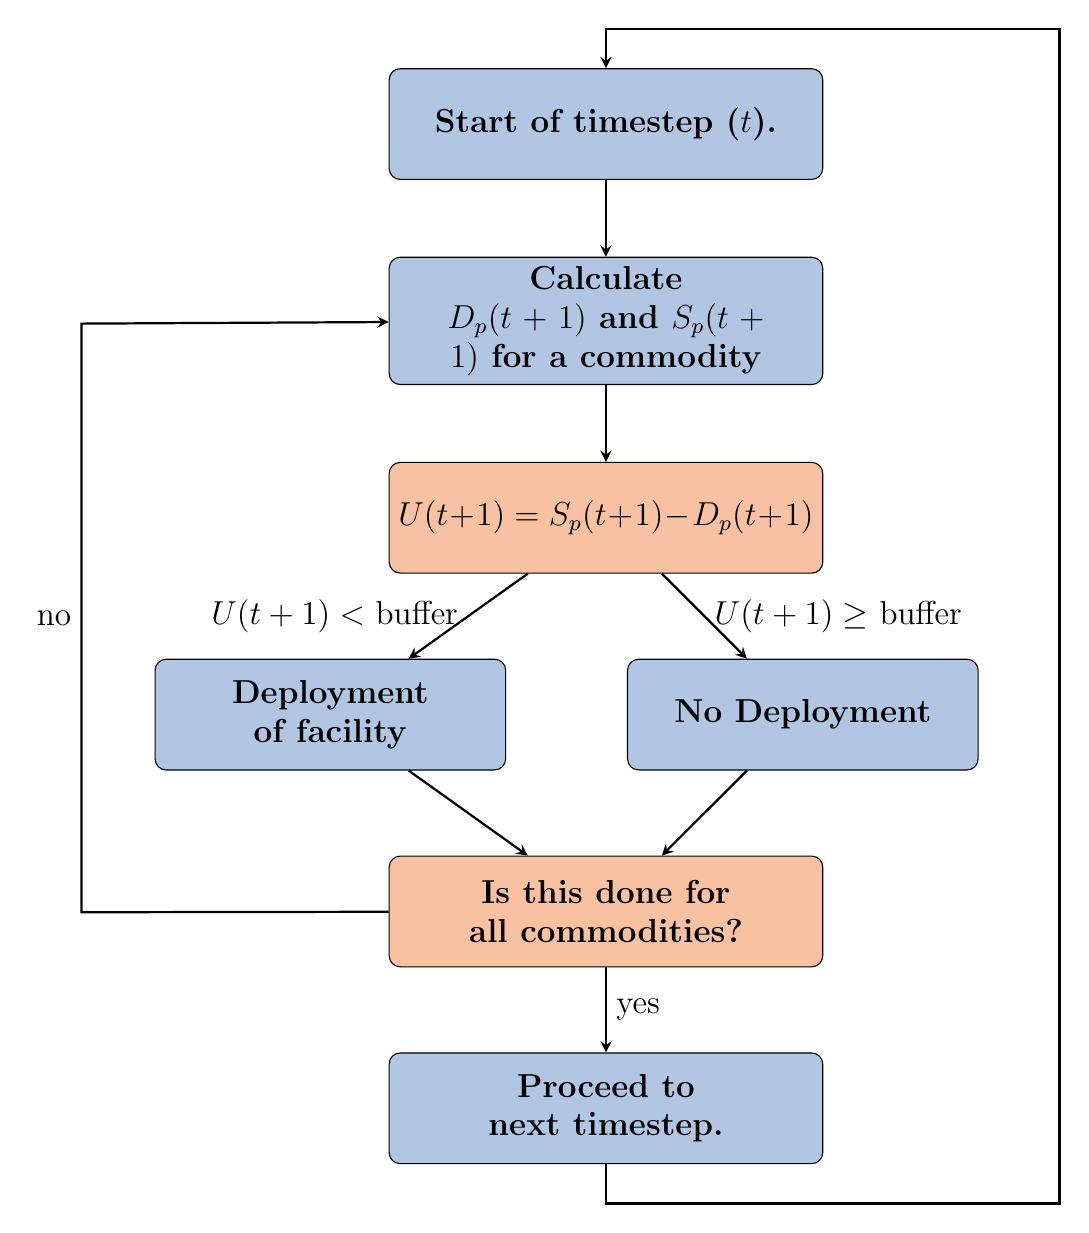
\begin{tikzpicture}[node distance=2.5cm]
        \tikzstyle{every node}=[font=\large]
        \node (Start) [bblock] {\textbf{Start of timestep ($t$).}};
        \node (Predict) [bblock, below of=Start] {\textbf{Calculate \\ $D_p(t+1)$ and $S_p(t+1)$ for a commodity}};
        \node (IsThere) [oblock, below of=Predict]{\textbf{$U(t+1) = S_p(t+1)-D_p(t+1)$}};
        \node (Deploy) [sbblock, below of=IsThere, xshift = -3.5cm]{\textbf{Deployment \\ of facility}};
        \node (NoDeploy) [sbblock, right of=Deploy, xshift = 3.5cm]{\textbf{No Deployment} };
        \node (All) [oblock, below of=Deploy, xshift = 3.5cm] {\textbf{Is this done for all commodities?}};
        \node (End) [bblock, below of=All] {\textbf{Proceed to next timestep.}};
        
        \draw [arrow] (Start) -- (Predict); 
        \draw [arrow] (Predict) -- (IsThere);
        \draw [arrow] (IsThere) -- node[anchor=east] {$U(t+1) <$ buffer} (Deploy);
        \draw [arrow] (IsThere) -- node[anchor=west] {$U(t+1) \geq$ buffer} (NoDeploy);
        \draw [arrow] (Deploy) -- (All);
        \draw [arrow] (NoDeploy) -- (All);
        \draw [arrow] (All) -- node[anchor=west] {yes} (End);
        \draw [arrow] (All) -- ([shift={(-3.9cm,0.7cm)}]All.south west)-- node[anchor=east] {no} ([shift={(-3.9cm,-0.85cm)}]Predict.north west)--(Predict);
        \draw [arrow] (End) |-([shift={(3cm,-0.5cm)}]End.south east)-- ([shift={(3cm,0.5cm)}]Start.north east)-|(Start);
    \end{tikzpicture}
\end{figure}

\deploy's overall objective is to ensure that there is no 
undersupply of power. 
The sub-objectives are : (1) to minimize the number of time 
steps of undersupply or under capacity of any 
commodity, (2): to minimize excessive oversupply of all commodities.
This is a reflection of reality in which it is important to 
never have an undersupply of power on the grid by ensuring power 
plants are never undersupplied of fuel, while not 
having excessive over supply resulting in a burden to store unused 
supplies. 
One of the key issues that \gls{NFCSim}s face is that despite
sufficient installed reactor capacity to meet the power 
demand, there is insufficient supply of fabricated/reprocessed 
fuel at certain timesteps, resulting in idle capacity.  

\subsubsection{\textbf{Structure}}
%Description of front end and back end of fuel cycle 
%Demand Driven vs. Supply Driven 
In \deploy, two different institutions were implemented for 
front-end and back-end fuel cycle facilities: 
\texttt{DemandDrivenDeploymentInst} and 
\texttt{SupplyDriven} 
\noindent
\texttt{DeploymentInst} respectively. 
This distinction was made because front-end facilities 
are deployed to meet demand for the commodity they produce. 
Whereas, back-end facility are deployed to meet supply for the 
commodity they provide capacity for. 
For example, for front end facilities, a reactor facility 
demands fuel and \texttt{DemandDrivenDeploymentInst} 
triggers deployment of fuel fabrication facilities to create 
supply meeting demand for fuel to prevent undersupply. 
For back end facilities, the reactor generates spent fuel and 
\texttt{SupplyDrivenDeploymentInst} triggers deployment of 
waste storage facilities to create capacity meeting the supply 
of spent fuel to prevent under capacity. 

\subsubsection{\textbf{Input Variables}}
Table \ref{tab:inputs} lists and gives examples of the input 
variables \deploy accepts. 
Essentially, the user must define the facilities controlled by 
\deploy, their respective capacities, the driving commodity, 
its demand equation, deployment driving method, and prediction method 
for supply and demand. 
The user also has the optional option to define supply/capacity buffers 
for each commodity, facility preferences, and facility constraints. 
In-depth descriptions of the deployment driving method, prediction 
methods, preferences, and buffers are provided in the subsequent sections. 

\begin{table}[]
    \centering
	\resizebox{0.7\textwidth}{!}{%
	\begin{tabular}{|l|l|p{7cm}|}
	\hline
											  & \textbf{Input Parameter}                                                           & \textbf{Examples}                                                                                                          \\ \hline
	\multirow{5}{*}{\textbf{Required}} & Demand driving commodity                                                           & Power, Fuel, Plutonium, etc.                                                                                                                      \\ \cline{2-3} 
											  & Demand equation                                                                    & P(t) = 10000, sin(t), 10000*t                                                                                                                 \\ \cline{2-3} 
											  & Facilities it controls                                                             & Fuel Fab, LWR reactor, SFR reactor, Waste repository, etc.                                                                                                      \\ \cline{2-3} 
											  & Capacities of the facilities                                                       & 3000 kg, 1000 MW, 50000 kg                                                                                                     \\ \cline{2-3} 
											  & Prediction method                                                                  & \begin{tabular}[c]{@{}l@{}}Power: fast fourier transform\\ Fuel: moving average\\ Spent fuel: moving average\end{tabular} \\ \cline{2-3} 
											  & Deployment driven by & Installed Capacity/Supply                                                                                                                    \\ \hline
	\multirow{4}{*}{\textbf{Optional}} & Supply/Capacity Buffer type                                                                        & Absolute                                                                                                                  \\ \cline{2-3} 
											  & Supply/Capacity Buffer size                                                                        & \begin{tabular}[c]{@{}l@{}}Power: 3000 MW\\ Fuel: 0 kg \\ Spent fuel: 0 kg\end{tabular}                                   \\ \cline{2-3} 
											  & Facility preferences                                                               & \begin{tabular}[c]{@{}l@{}}LWR reactor = 100-t\\ SFR reactor = t-100 \end{tabular}          \\ \cline{2-3} 
											  & Facility constraint                                                              & SFR reactor constraint = 5000kg of Pu            \\ \hline	
			
											\end{tabular}%
	}
	\caption{\deploy's required and optional input parameters with examples.}
	\label{tab:inputs}
    \end{table}

    \subsubsection{\textbf{Deployment Driving Method}}
    The user has the choice of deploying facilities based on the difference 
    between predicted supply and demand, or predicted demand and 
    installed capacity. 
    There are two advantages of using installed capacity over predicted 
    supply. 
    First, to prevent over deployment of facilities that have an
    intermittent supply. 
    For example, reactor facilities have a periodic refueling time. 
    A user might not want \deploy to deploy more reactor facilities 
    to make up for the lack of power supply caused by the gap in 
    supply during refueling. 
    Second, to prevent infinite deployment of a facility that uses 
    a commodity that is no longer available in the simulation. 
    For example, in a transition scenario from \gls{LWR}s to \gls{SFR}s, 
    the reprocessing plant that fabricates \gls{SFR} fuel might demand 
    Pu after the inventory accumulated by \gls{LWR}s is used up 
    and there are no more \gls{LWR} facilities to generate Pu. 
    This will result in \deploy deploying infinite reprocessing 
    facilities to generate \gls{SFR} fuel despite the lack of input Pu 
    to generate it. 
    This can be avoided by using \deploy's facility constraint capability 
    to constrain \gls{SFR} deployment until a sizable inventory of Pu 
    is accumulated in the simulation. 
    
    \subsubsection{\textbf{Supply/Capacity Buffer}}
    In \texttt{DemandDrivenDeploymentInst}, the user has the option 
    to provide a supply buffer for each commodity so that 
    \deploy will deploy facilities to meet predicted demand and the
    additional buffer value. 
    In \texttt{SupplyDrivenDeploymentInst}, the user has the option 
    to provide a capacity buffer to specific commodities so that 
    \deploy will deploy facilities to meet predicted supply and the
    additional buffer.
    For example, the user could set the power commodity's supply buffer 
    to be 2000 MW. 
    If predicted demand is 10000 MW, \deploy will deploy reactor 
    facilities to meet the predicted demand and supply buffer, resulting 
    in a power supply of 12000 MW.  
    The buffer can be defined as a percentage (equation \ref{eq:perc}) 
    or absolute value (equation \ref{eq:abs}). 
    
    \begin{equation}
        \label{eq:perc}
        S_{pwb} = S_{p}*(1+d)
    \end{equation}
    \begin{equation}
        \label{eq:abs}
        S_{pwb} = S_{p}+a
    \end{equation}
    where $S_{pwb}$ is predicted supply/capacity with buffer, 
    $S_p$ is the predicted supply/capacity without buffer, 
    $d$ is the percentage value in decimal form, 
    and $a$ is the absolute value of the buffer. 
    
    Using a combination of this buffer capability with the 
    installed capacity deployment driving method in a transition 
    scenario simulation is effective in minimizing undersupply of a 
    commodity without having excessive over supply. 
    This is demonstrated in section \ref{sec:demo}. 
    
    \subsubsection{\textbf{Preferences}}
    % Need to explain the order of preferences for deployment 
    % Constraint, pref, minimize number of facilities and minimize 
    % over supply 
    The user has the option to provide each facility with
    a time dependent preference equation that governs preference for 
    that facility compared to other facilities that provide the same 
    commodity. 
    In the example for facility preferences in table \ref{tab:inputs}, 
    the \gls{LWR} reactor has a preference of $100-t$ and the 
    \gls{SFR} reactor has a preference of $t-100$. 
    Thus, the \gls{LWR} is preferred before time step 100 and \gls{SFR}
    is preferred after. 
    
    The user also has the option to provide each facility with a 
    commodity constraint. 
    In the example for facility constraint in table \ref{tab:inputs}, 
    the \gls{SFR} has a commodity constraint of 5000kg of Pu. 
    This constrains \gls{SFR} deployment by the size of the Pu inventory 
    in the simulation. 
    Once, the 5000kg Pu inventory is first met, \gls{SFR} reactors can 
    henceforth be deployed. 
    
    One of the key issues faced in transition scenarios is the lack 
    of Pu in a scenario that results in idle advanced reactor capacity. 
    Therefore, the facility preferences and constraint capabilities 
    are useful and necessary for modeling transition scenarios. 
    An ideal transition year is selected using the facility 
    preferences, however the transition will only begin when there 
    is sufficient Pu inventory (set by facility constraint) 
    to avoid Pu shortages. 
    
    Therefore, when \deploy predicts an undersupply of a commodity, 
    it deploys available facilities to meet the predicted demand. 
    It will deploy the facility with the highest preference first, 
    unless it does not meet it's constrained criteria, then it will 
    deploy the second most, and so on. 
    If the facilities do not have preferences or constraints, \deploy 
    will deploy the available facilities to minimize the number of 
    deployed facilities while minimizing oversupply of the commodity.

\subsubsection{\textbf{Prediction Methods}}

\subsection{\deploy Demonstration}
\label{sec:demo}

This section will demonstrate \deploy's capability 
to effectively conduct simple transition scenario analysis
for constant, linearly increasing, and 
sinusoidal power demand simulations.
These simulations are basic transition scenarios that only include 
three types of facilities: \texttt{source}, \texttt{reactor}, and 
\texttt{sink}. 
All simulations have ten initial \texttt{reactor} facilities 
(\texttt{reactor1} to \texttt{reactor10}). 
These reactors have staggered cycle lengths and lifetimes to prevent 
simultaneous refueling and set up gradual decommissioning. 
\deploy is set up to deploy \texttt{new reactor} facilities
to meet the loss of power supply introduced from the decommissioning 
of the initial \texttt{reactor} facilities. 
The \deploy input parameters for each simulation is shown in Table 
\ref{tab:demonstrations}. 
Figure \ref{fig:powerplots} shows the user-defined power demand curves 
that \deploy needs to deploy facilities meet for each simulation.

\begin{table}[]
    \resizebox{\textwidth}{!}{%
    \begin{tabular}{|l|l|c|l|l|}
    \hline
    \multirow{2}{*}{}                         & \multicolumn{1}{c|}{\multirow{2}{*}{\textbf{Input Parameter}}} & \multicolumn{3}{c|}{\textbf{Simulation Description}}                                                                                                                                                                                                                                                       \\ \cline{3-5} 
                                              & \multicolumn{1}{c|}{}                                          & \multicolumn{1}{l|}{\textbf{Constant Power}}                                                                 & \textbf{\begin{tabular}[c]{@{}l@{}}Linearly Increasing \\ Power\end{tabular}}                  & \textbf{Sinusoidal Power}                                                                  \\ \hline
    \multirow{5}{*}{\textbf{Required Inputs}} & Demand driving commodity                                       & \multicolumn{3}{c|}{Power}                                                                                                                                                                                                                                                                                 \\ \cline{2-5} 
                                              & Demand equation                                                & \multicolumn{1}{l|}{10000 MW}                                                                                & \begin{tabular}[c]{@{}l@{}}t\textless 40: 10000 MW\\ t\textgreater{}=40: 250*t MW\end{tabular} & 1000*$\sin(\pi*t/3)$+10000                                                                 \\ \cline{2-5} 
                                              & Facilities it controls                                         & \multicolumn{3}{c|}{Source, reactor, sink}                                                                                                                                                                                                                                                                 \\ \cline{2-5} 
                                              & Prediction method                                              & \multicolumn{1}{l|}{\begin{tabular}[c]{@{}l@{}}Power: FFT\\ Fuel: MA\\ Spent fuel: MA\end{tabular}}          & \begin{tabular}[c]{@{}l@{}}Power: FFT\\ Fuel: MA\\ Spent fuel: FFT\end{tabular}                & \begin{tabular}[c]{@{}l@{}}Power: HW\\ Fuel: MA\\ Spent fuel: FFT\end{tabular}             \\ \cline{2-5} 
                                              & Deployment Driving Method                                      & \multicolumn{3}{c|}{Installed Capacity}                                                                                                                                                                                                                                                                    \\ \hline
    \multirow{2}{*}{\textbf{Optional Inputs}} & Buffer type                                                    & \multicolumn{3}{c|}{Absolute}                                                                                                                                                                                                                                                                              \\ \cline{2-5} 
                                              & Buffer size                                                    & \multicolumn{1}{l|}{\begin{tabular}[c]{@{}l@{}}Power: 3000 MW\\ Fuel: 0 kg \\ Spent fuel: 0 kg\end{tabular}} & \begin{tabular}[c]{@{}l@{}}Power: 2000 MW\\ Fuel: 1000 kg \\ Spent fuel: 0 kg\end{tabular}     & \begin{tabular}[c]{@{}l@{}}Power: 2000 MW\\ Fuel: 1000 kg \\ Spent fuel: 0 kg\end{tabular} \\ \hline
    \end{tabular}%
    }
    \caption{\deploy's input parameters for the basic transition scenarios.}
    \label{tab:demonstrations}
    \end{table}

    \begin{figure}[]
        \begin{center}
            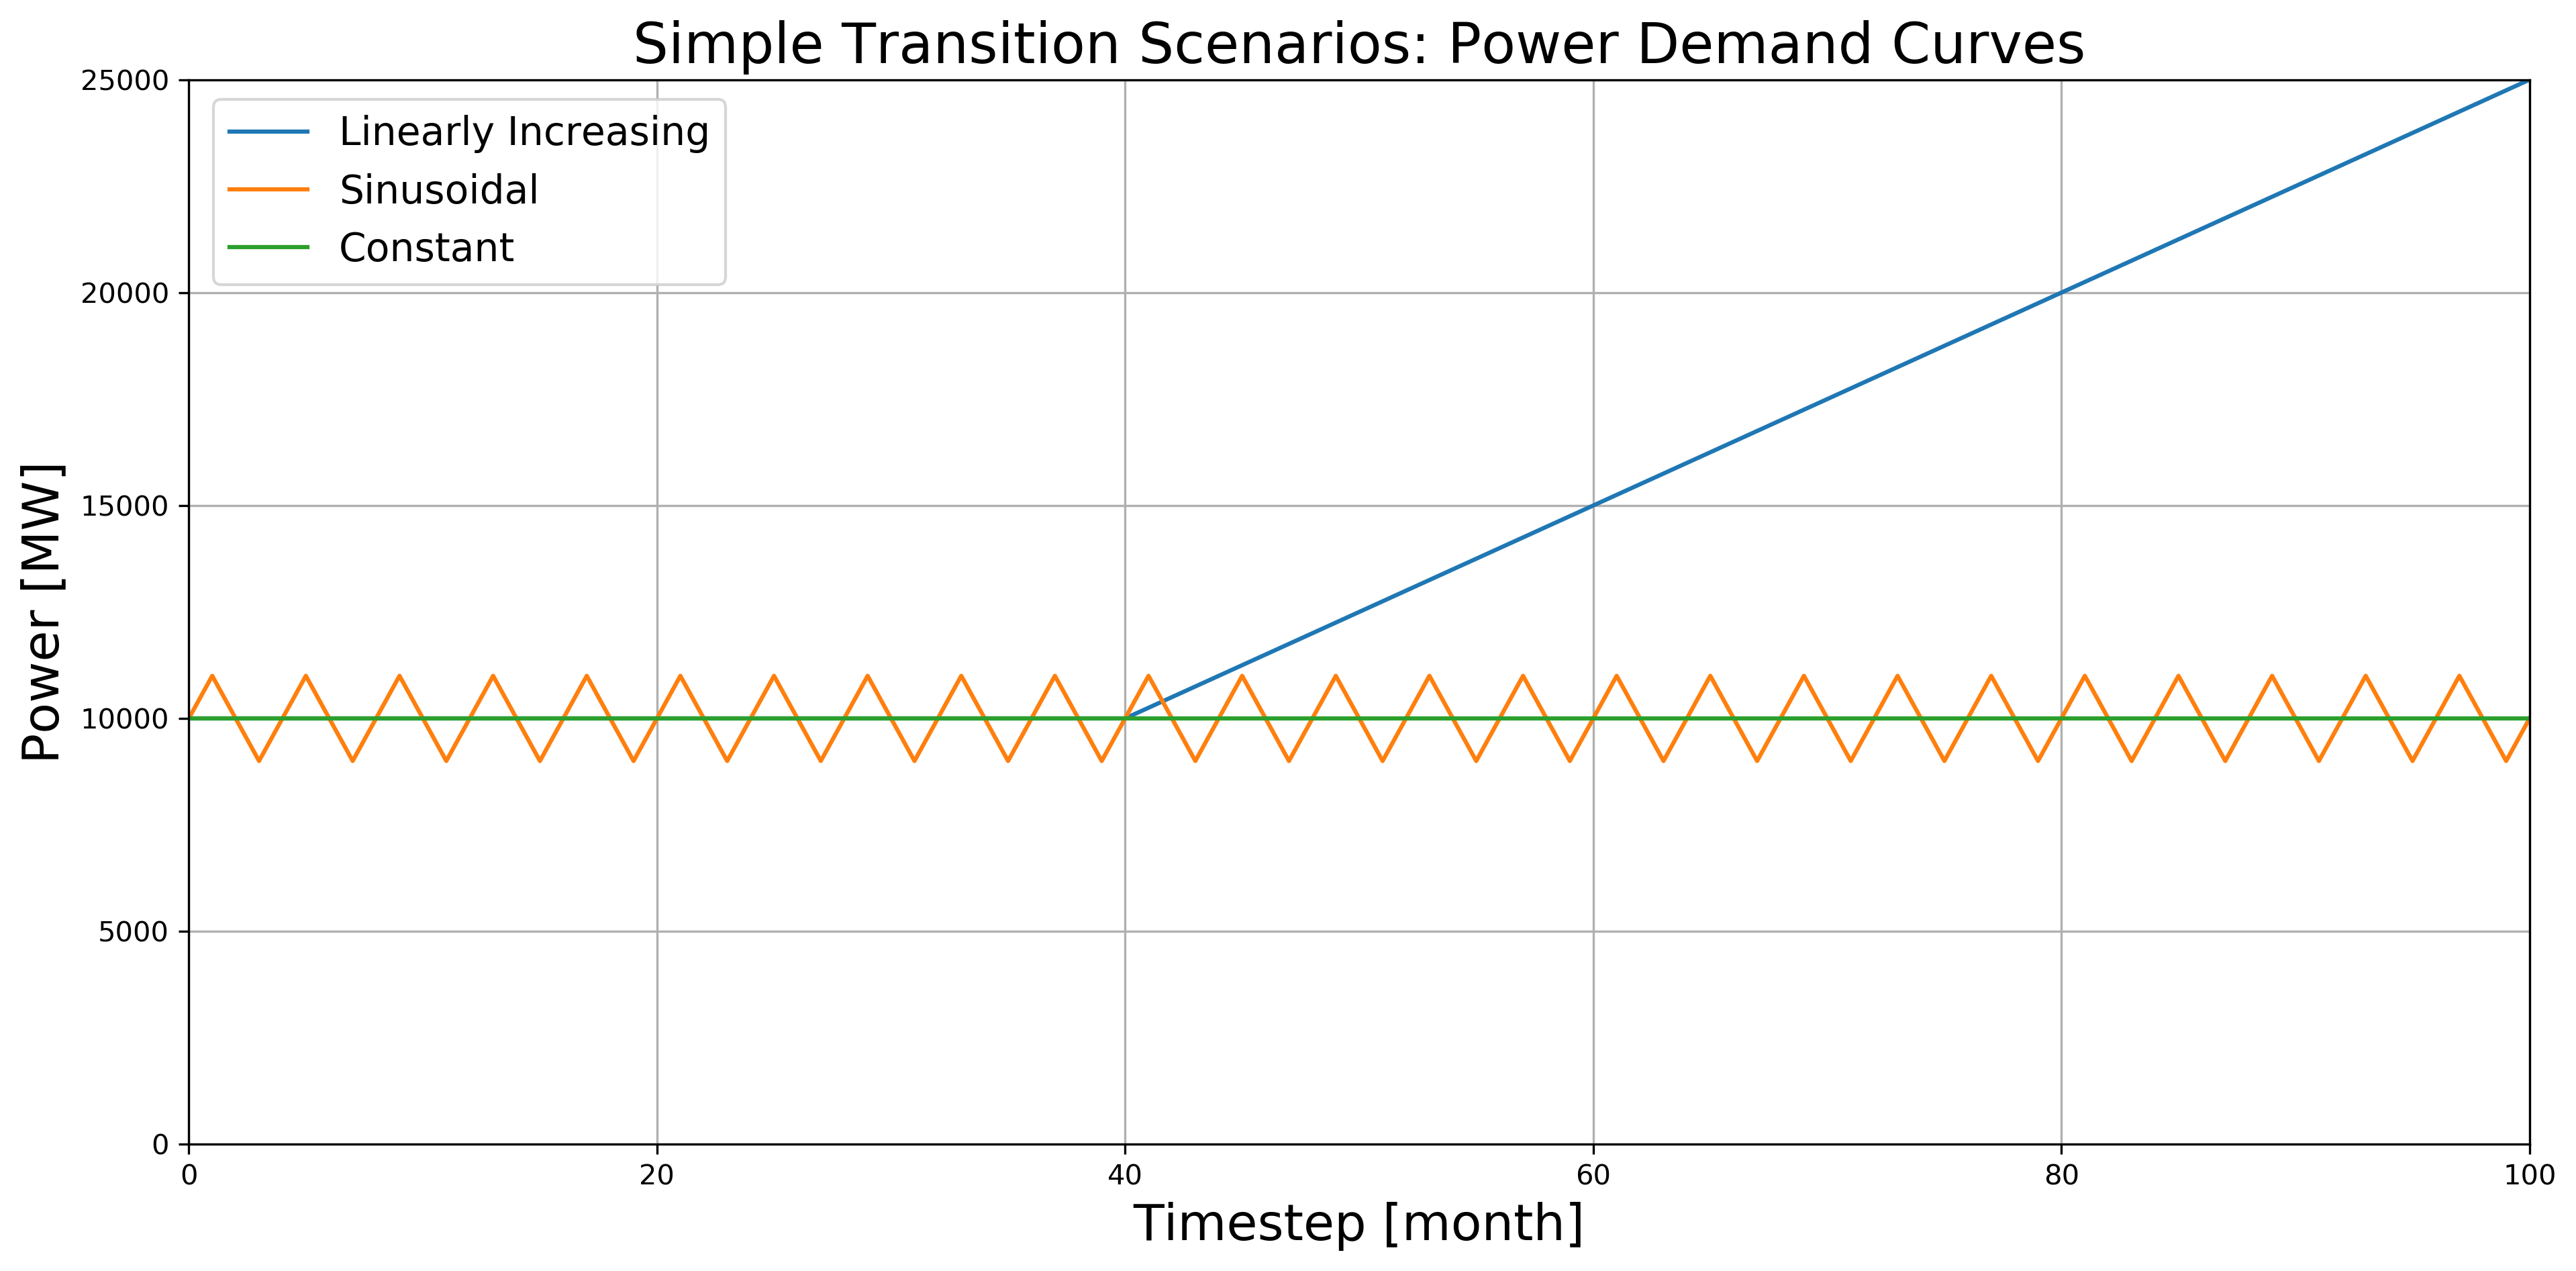
\includegraphics[scale=0.37]{./figures/powerplots.png}
        \end{center}
            \caption{Power demand curves for basic transition scenarios.}
        \label{fig:powerplots}
    \end{figure}

\subsubsection{\textbf{Basic Transition Scenario Simulation: Constant Demand}}
Figures \ref{fig:constanttransition-power}, \ref{fig:constanttransition-fuel}
and \ref{fig:constanttransition-spentfuel} demonstrate \deploy's capability 
to deploy reactor and supporting facilities to meet the user 
determined constant power demand and subsequently demanded 
secondary commodities with minimal undersupply. 
Table \ref{tab:transition-scenario-results} shows the number of 
undersupplied timesteps. 
Figure \ref{fig:constanttransition-power} demonstrates that
the main objective of \deploy (section \ref{sec:d3ploy}) 
was met since there are no timesteps
in which the supply of power falls under demand.
By using a combination of the fast fourier transform method for 
predicting demand and setting the supply buffer to 3000MW 
(the capacity of 3 reactors), the user minimizes the number of 
undersupplied timesteps for every commodity.

In figure \ref{fig:constanttransition-fuel},
a facility with a large fuel throughput is initially
deployed to meet the large initial fuel demand for the starting
up of ten reactors. 
\deploy is prevented from deploying many supporting
facilities that end up being redundant at the later parts of 
the simulation, by having an initial facility with a large throughput
exist for the first few timesteps in the simulation.
This is a reflection of reality in which reactor manufacturers will 
accumulate an appropriate amount of fuel inventory before starting 
up reactors. 
There is one timestep where there is an undersupply after the 
decommissioning of the large initial facility.  
This is unavoidable since the prediction methods in \deploy are 
unable to predict this sudden drop in demand. 

    \begin{figure}[]
        \centering
        \begin{subfigure}[t]{\textwidth}
        \centering
            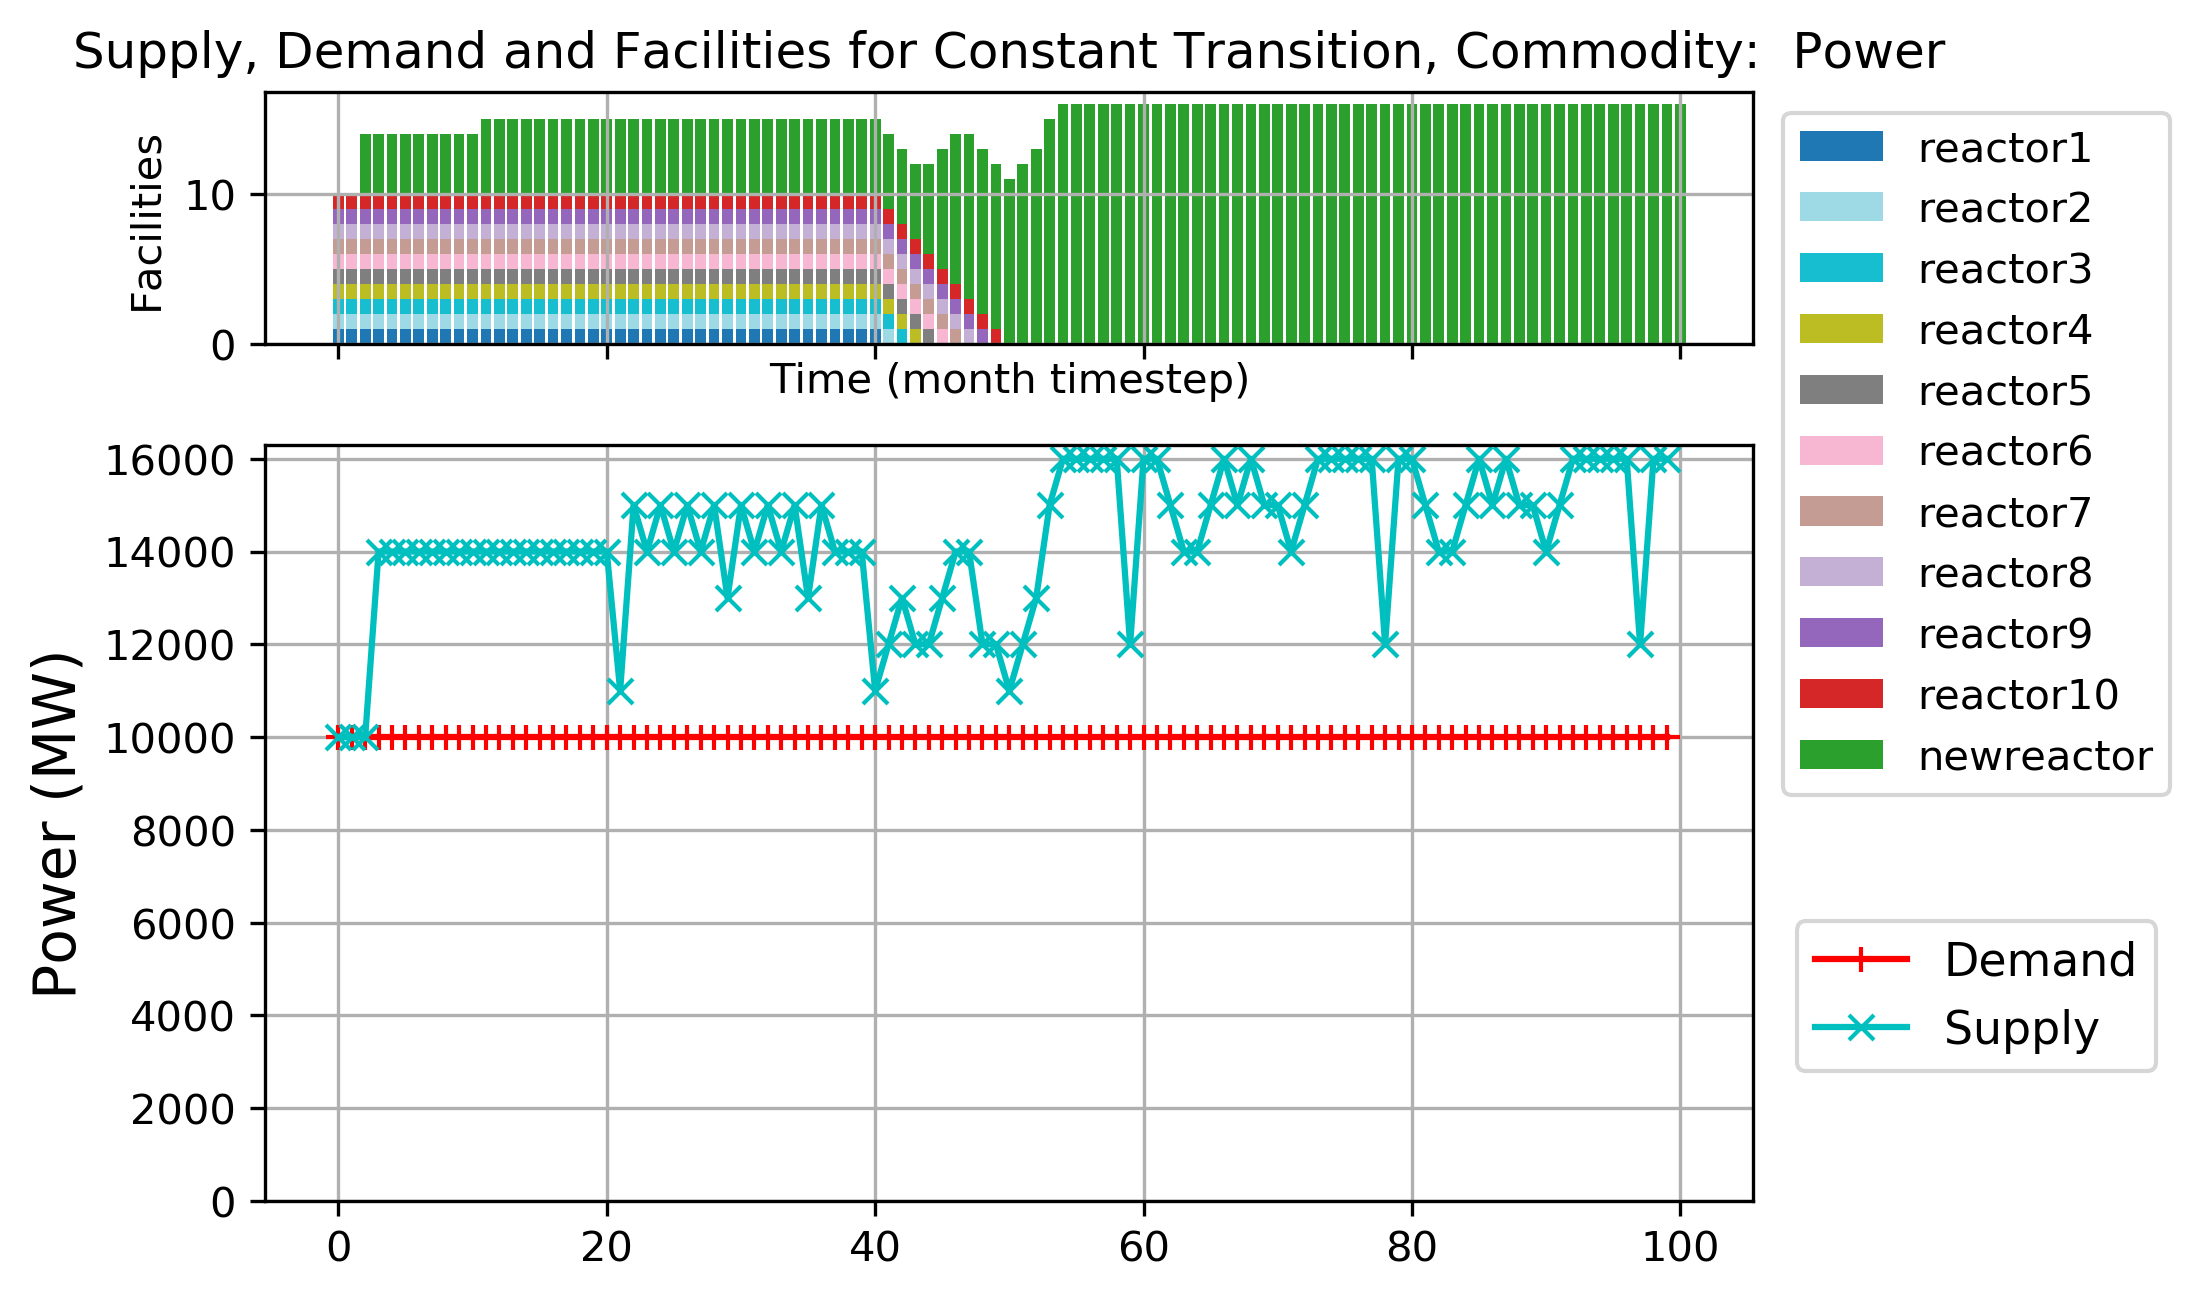
\includegraphics[width=0.7\linewidth]{figures/constanttransition-power.png} 
            \caption{The power demand is a user-defined equation and power is supplied by the reactors.}
            \label{fig:constanttransition-power}
        \end{subfigure}
        \begin{subfigure}[t]{0.6\textwidth}
            \centering
            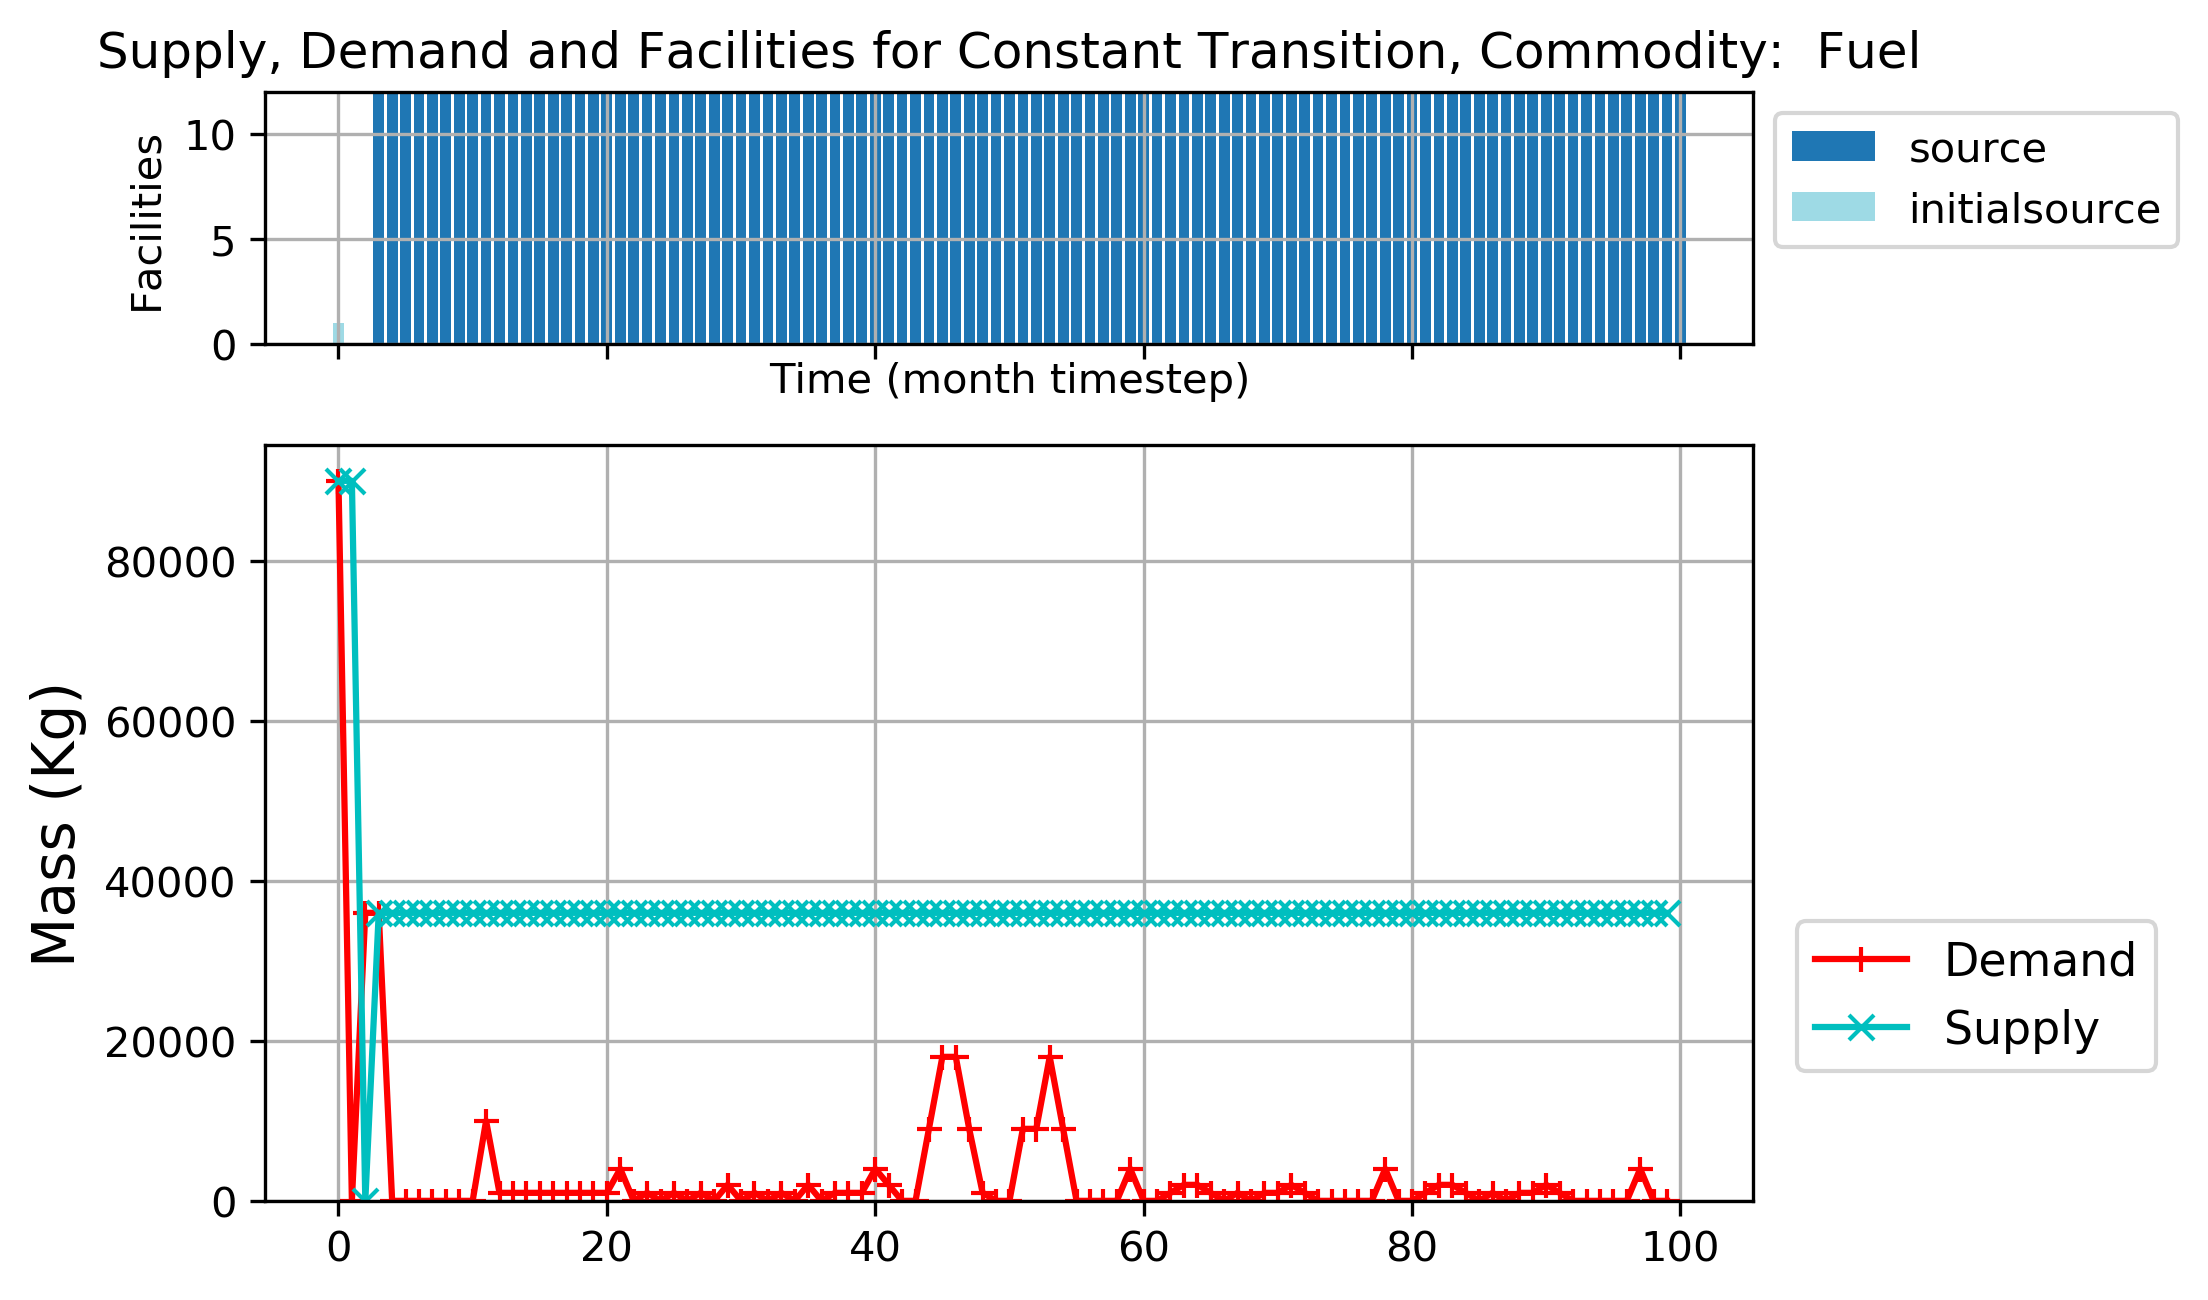
\includegraphics[width=\linewidth]{figures/constanttransition-fuel.png} 
            \caption{Fuel is demanded by reactors and supplied by source facilities.}
            \label{fig:constanttransition-fuel}
        \end{subfigure}
        \begin{subfigure}[t]{0.6\textwidth}
            \centering
            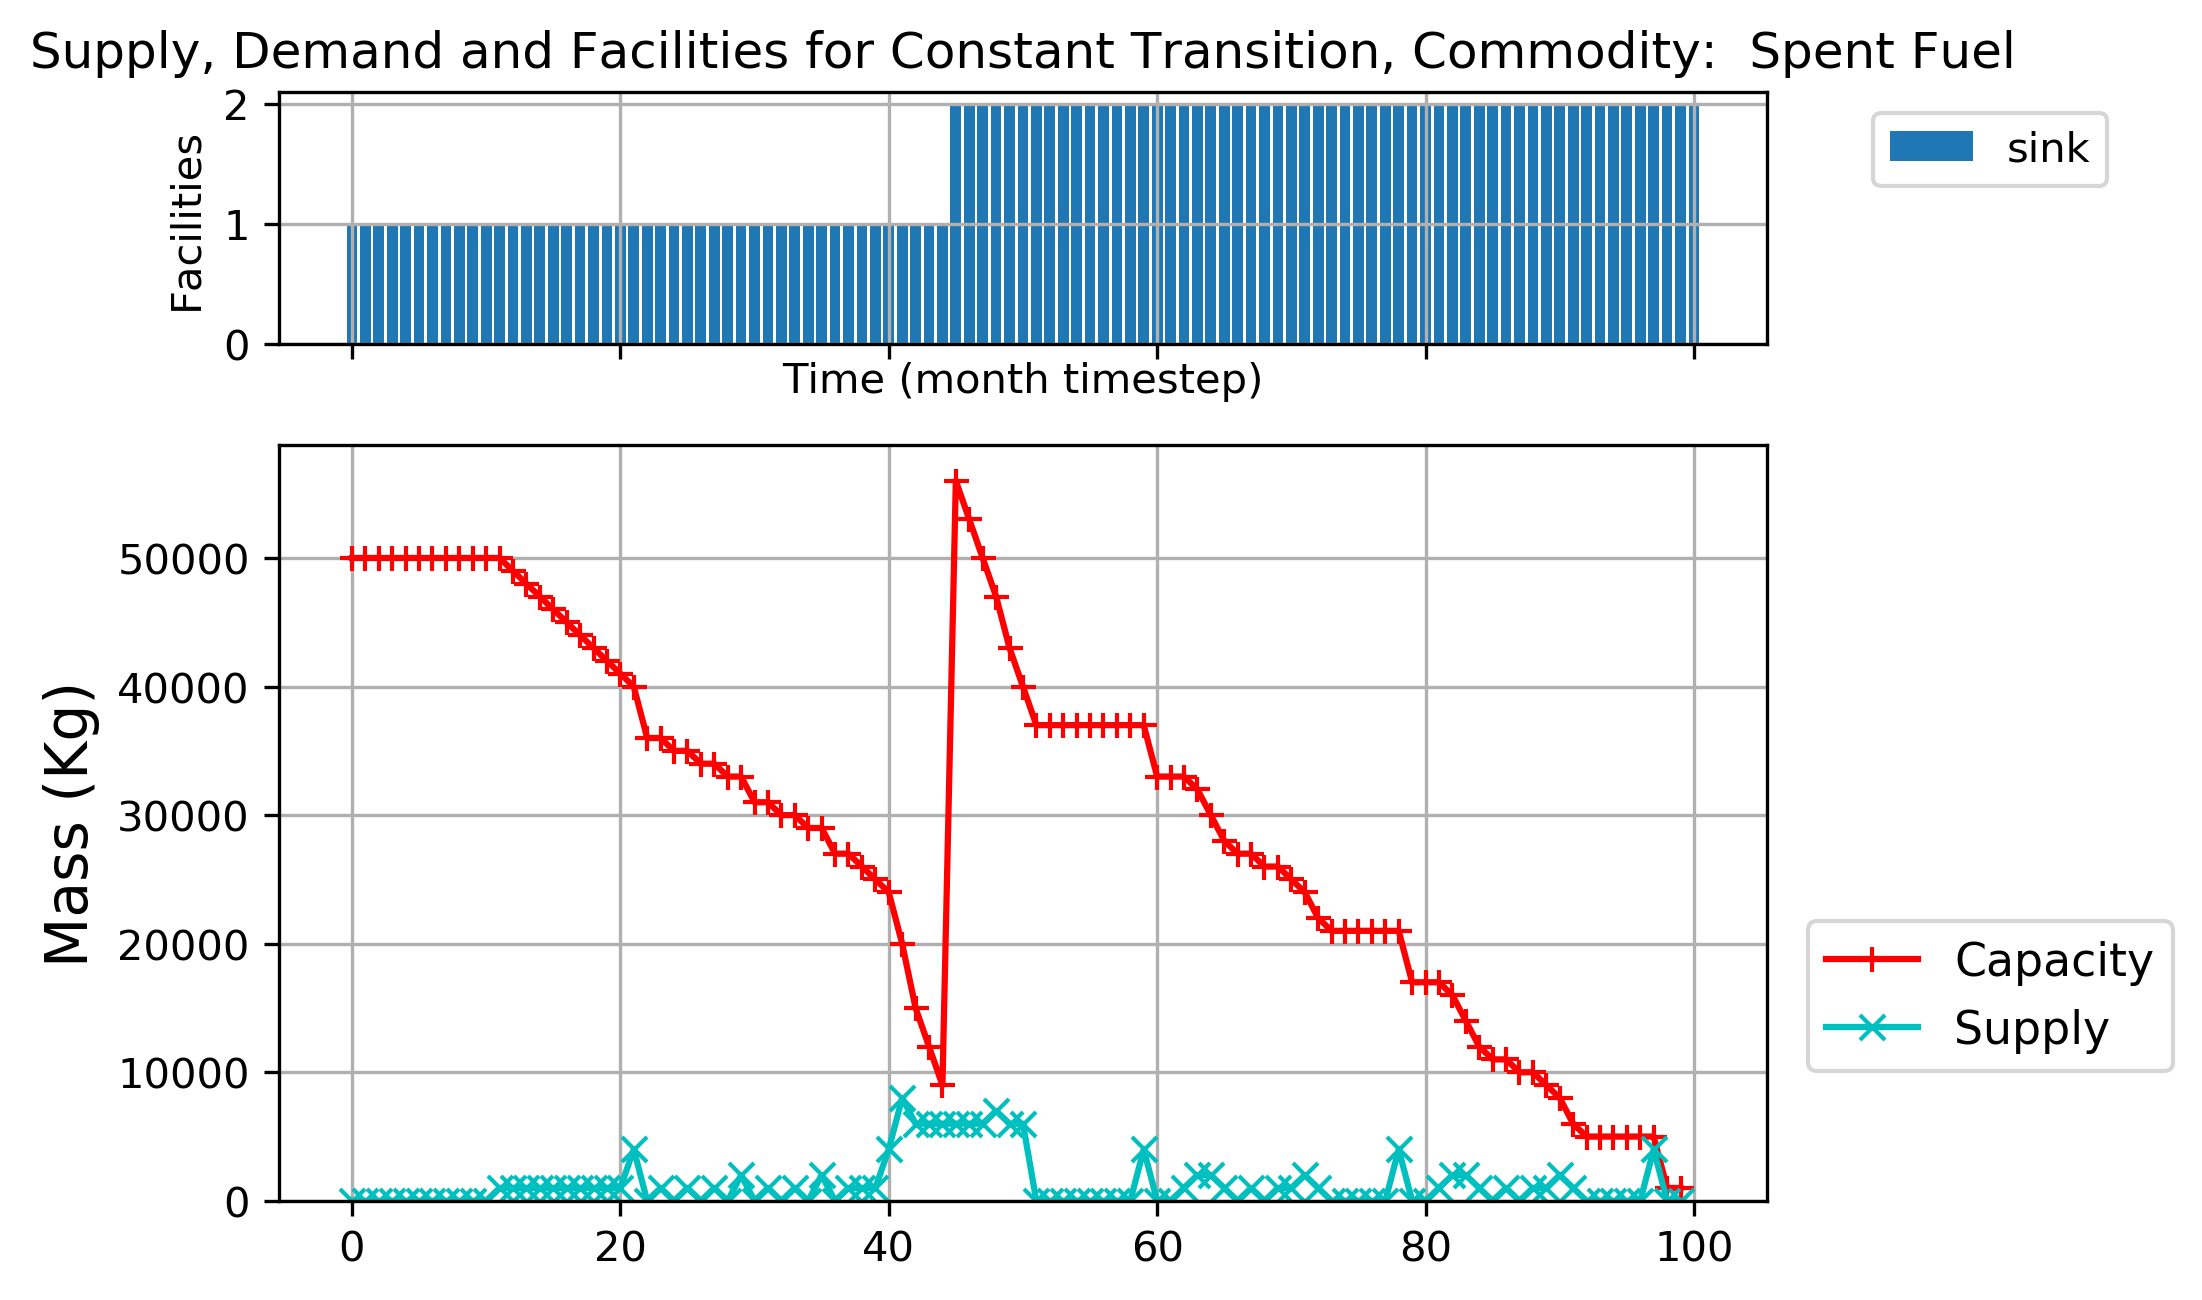
\includegraphics[width=\linewidth]{figures/constanttransition-spentfuel.png} 
            \caption{Spent Fuel is supplied by reactors and the capacity is provided by sink facilities.}
            \label{fig:constanttransition-spentfuel}
        \end{subfigure}
        \caption{Transition Scenario: Constant Power Demand of 10000MW}
    \end{figure}

    \subsubsection{\textbf{Basic Transition Scenario Simulation: Linearly Increasing Demand}}

    Figures \ref{fig:growingtransition-power}, \ref{fig:growingtransition-fuel}
    and \ref{fig:growingtransition-spentfuel} demonstrate the capability 
    of \deploy to deploy reactor and supporting facilities to meet the
    power demand and subsequently demanded secondary commodities 
    for a linearly increasing power demand. 
    A smaller supply buffer could be used while still minimizing under supply.
    Table \ref{tab:transition-scenario-results} shows the number of 
    undersupplied timesteps. 
    Figure \ref{fig:growingtransition-power} demonstrates that
    the main objective of \deploy (section \ref{sec:d3ploy}) 
    was met since there are no timesteps
    in which the supply of power falls under demand.
    
    \begin{figure}[]
        \centering
        \begin{subfigure}[t]{\textwidth}
        \centering
            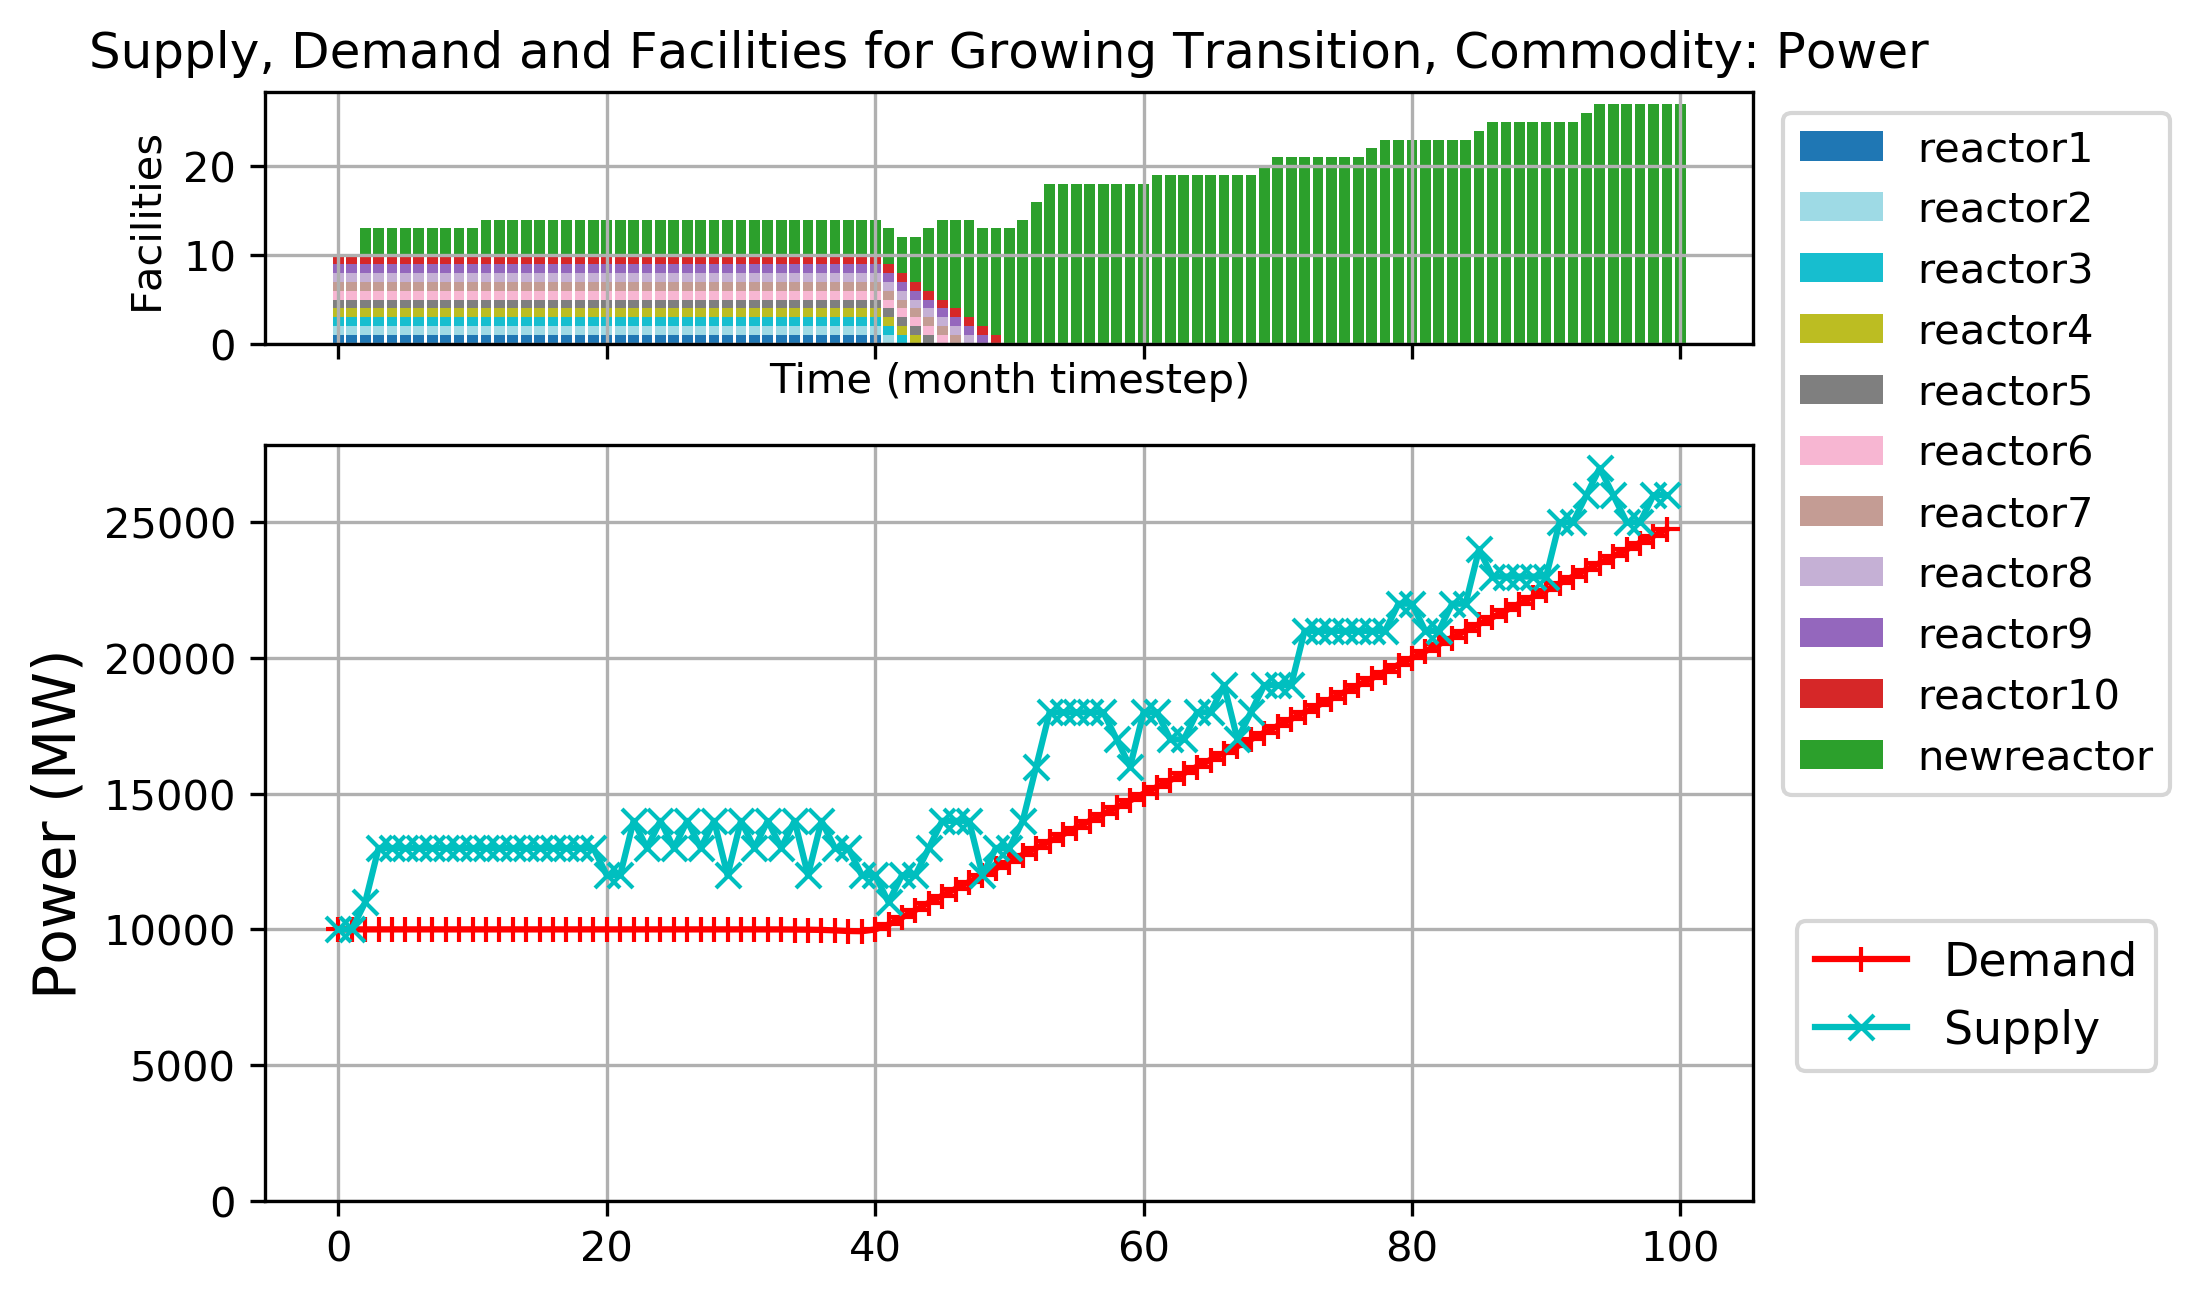
\includegraphics[width=0.7\linewidth]{figures/growingtransition-power.png} 
            \caption{The power demand is a user-defined equation and power is supplied by the reactors.}
            \label{fig:growingtransition-power}
        \end{subfigure}
        \begin{subfigure}[t]{0.6\textwidth}
            \centering
            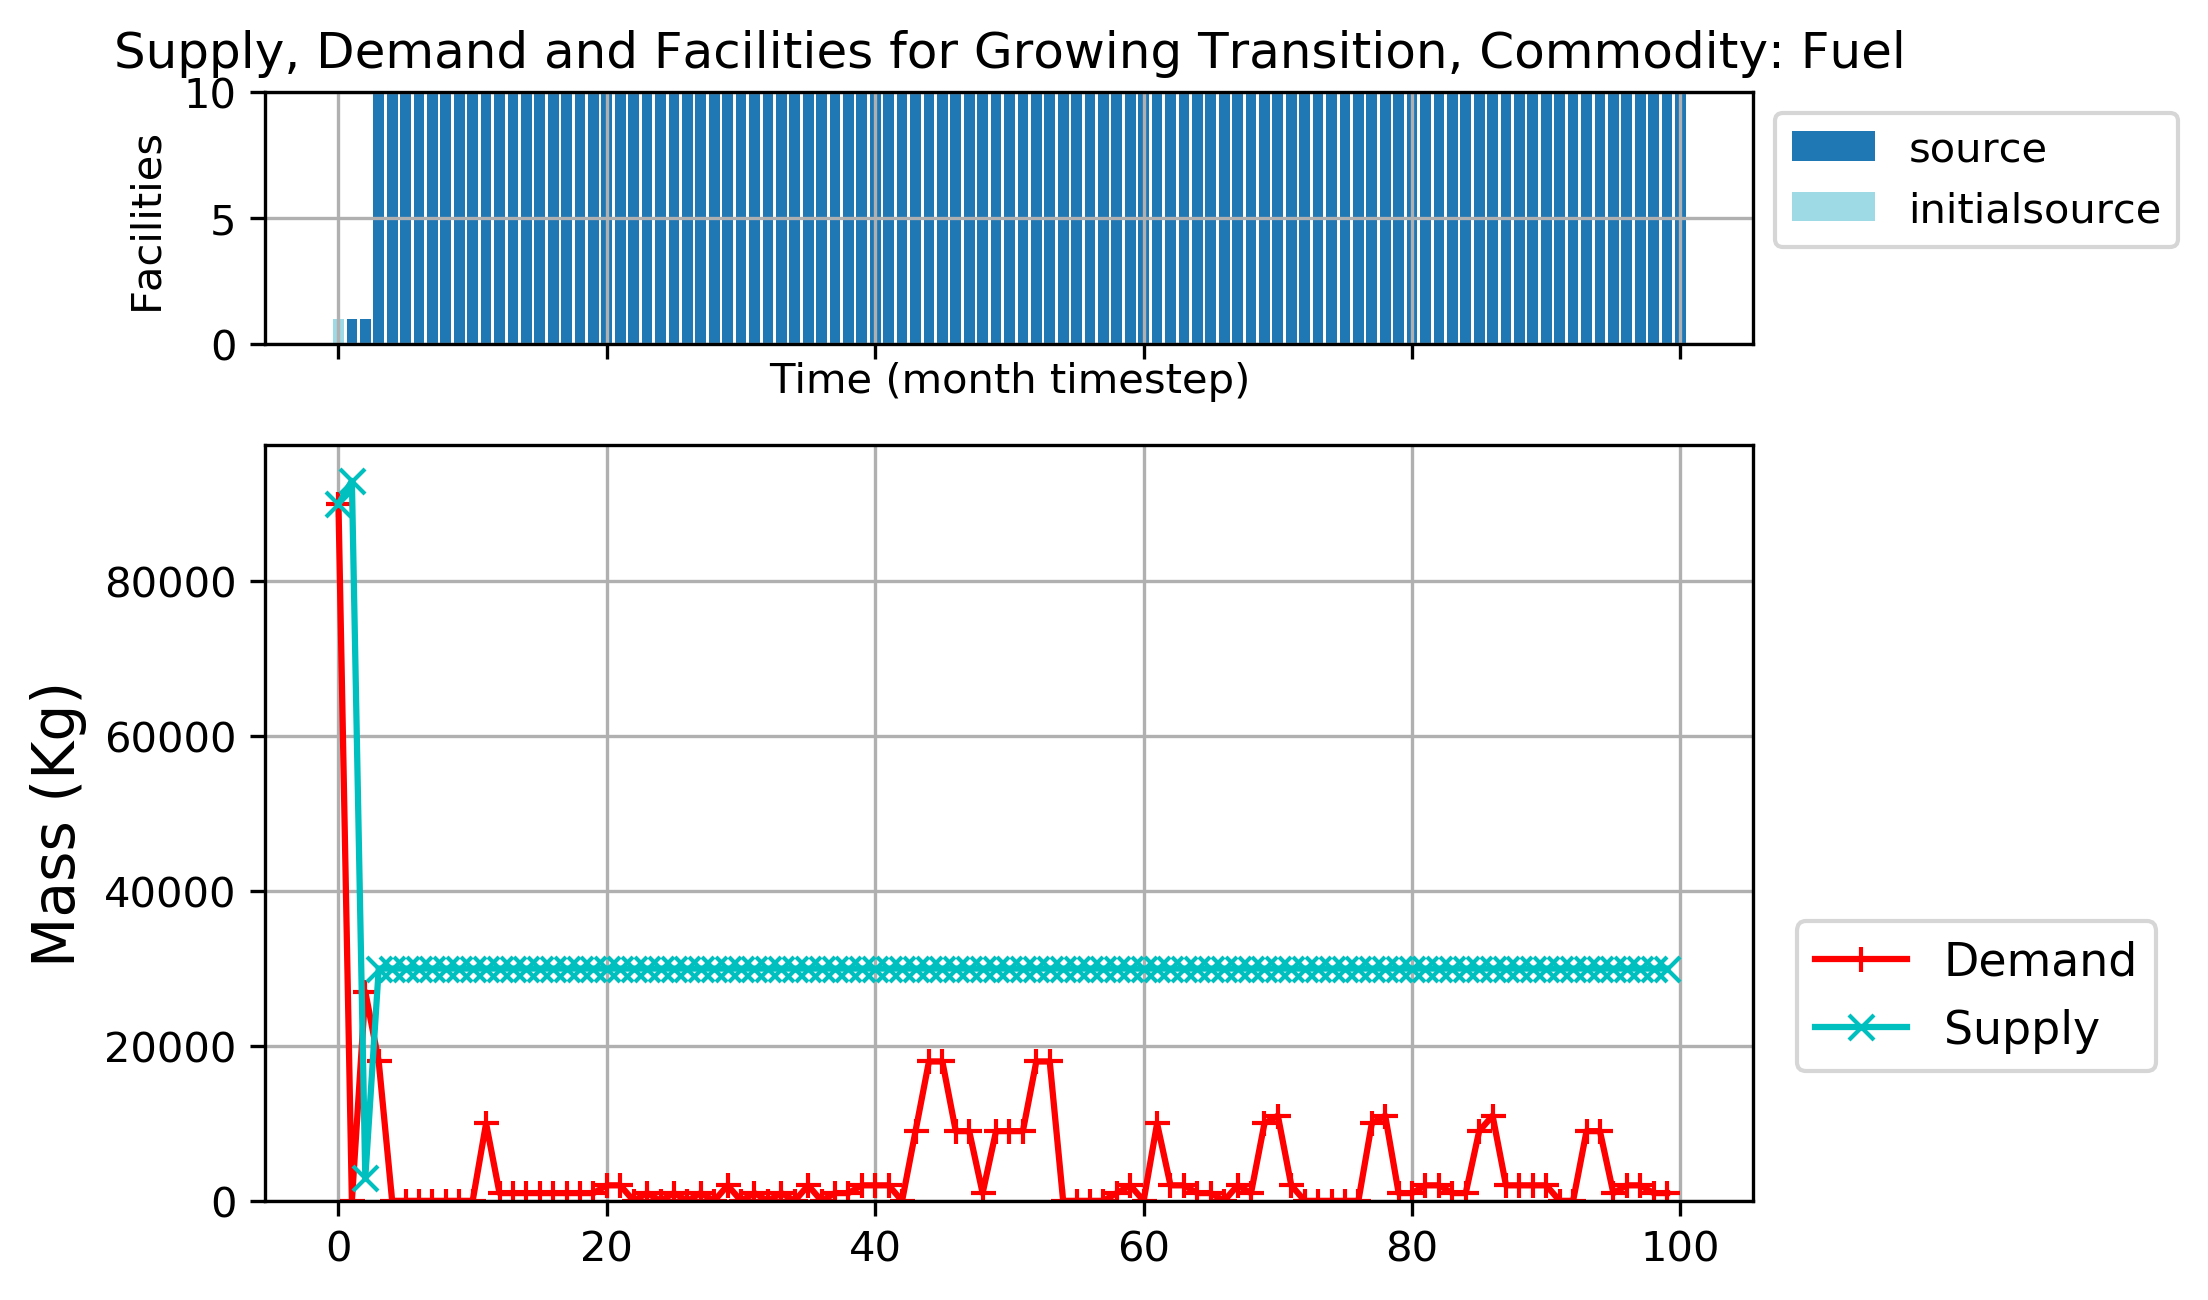
\includegraphics[width=\linewidth]{figures/growingtransition-fuel.png} 
            \caption{Fuel is demanded by reactors and supplied by source facilities.}
            \label{fig:growingtransition-fuel}
        \end{subfigure}
        \begin{subfigure}[t]{0.6\textwidth}
            \centering
            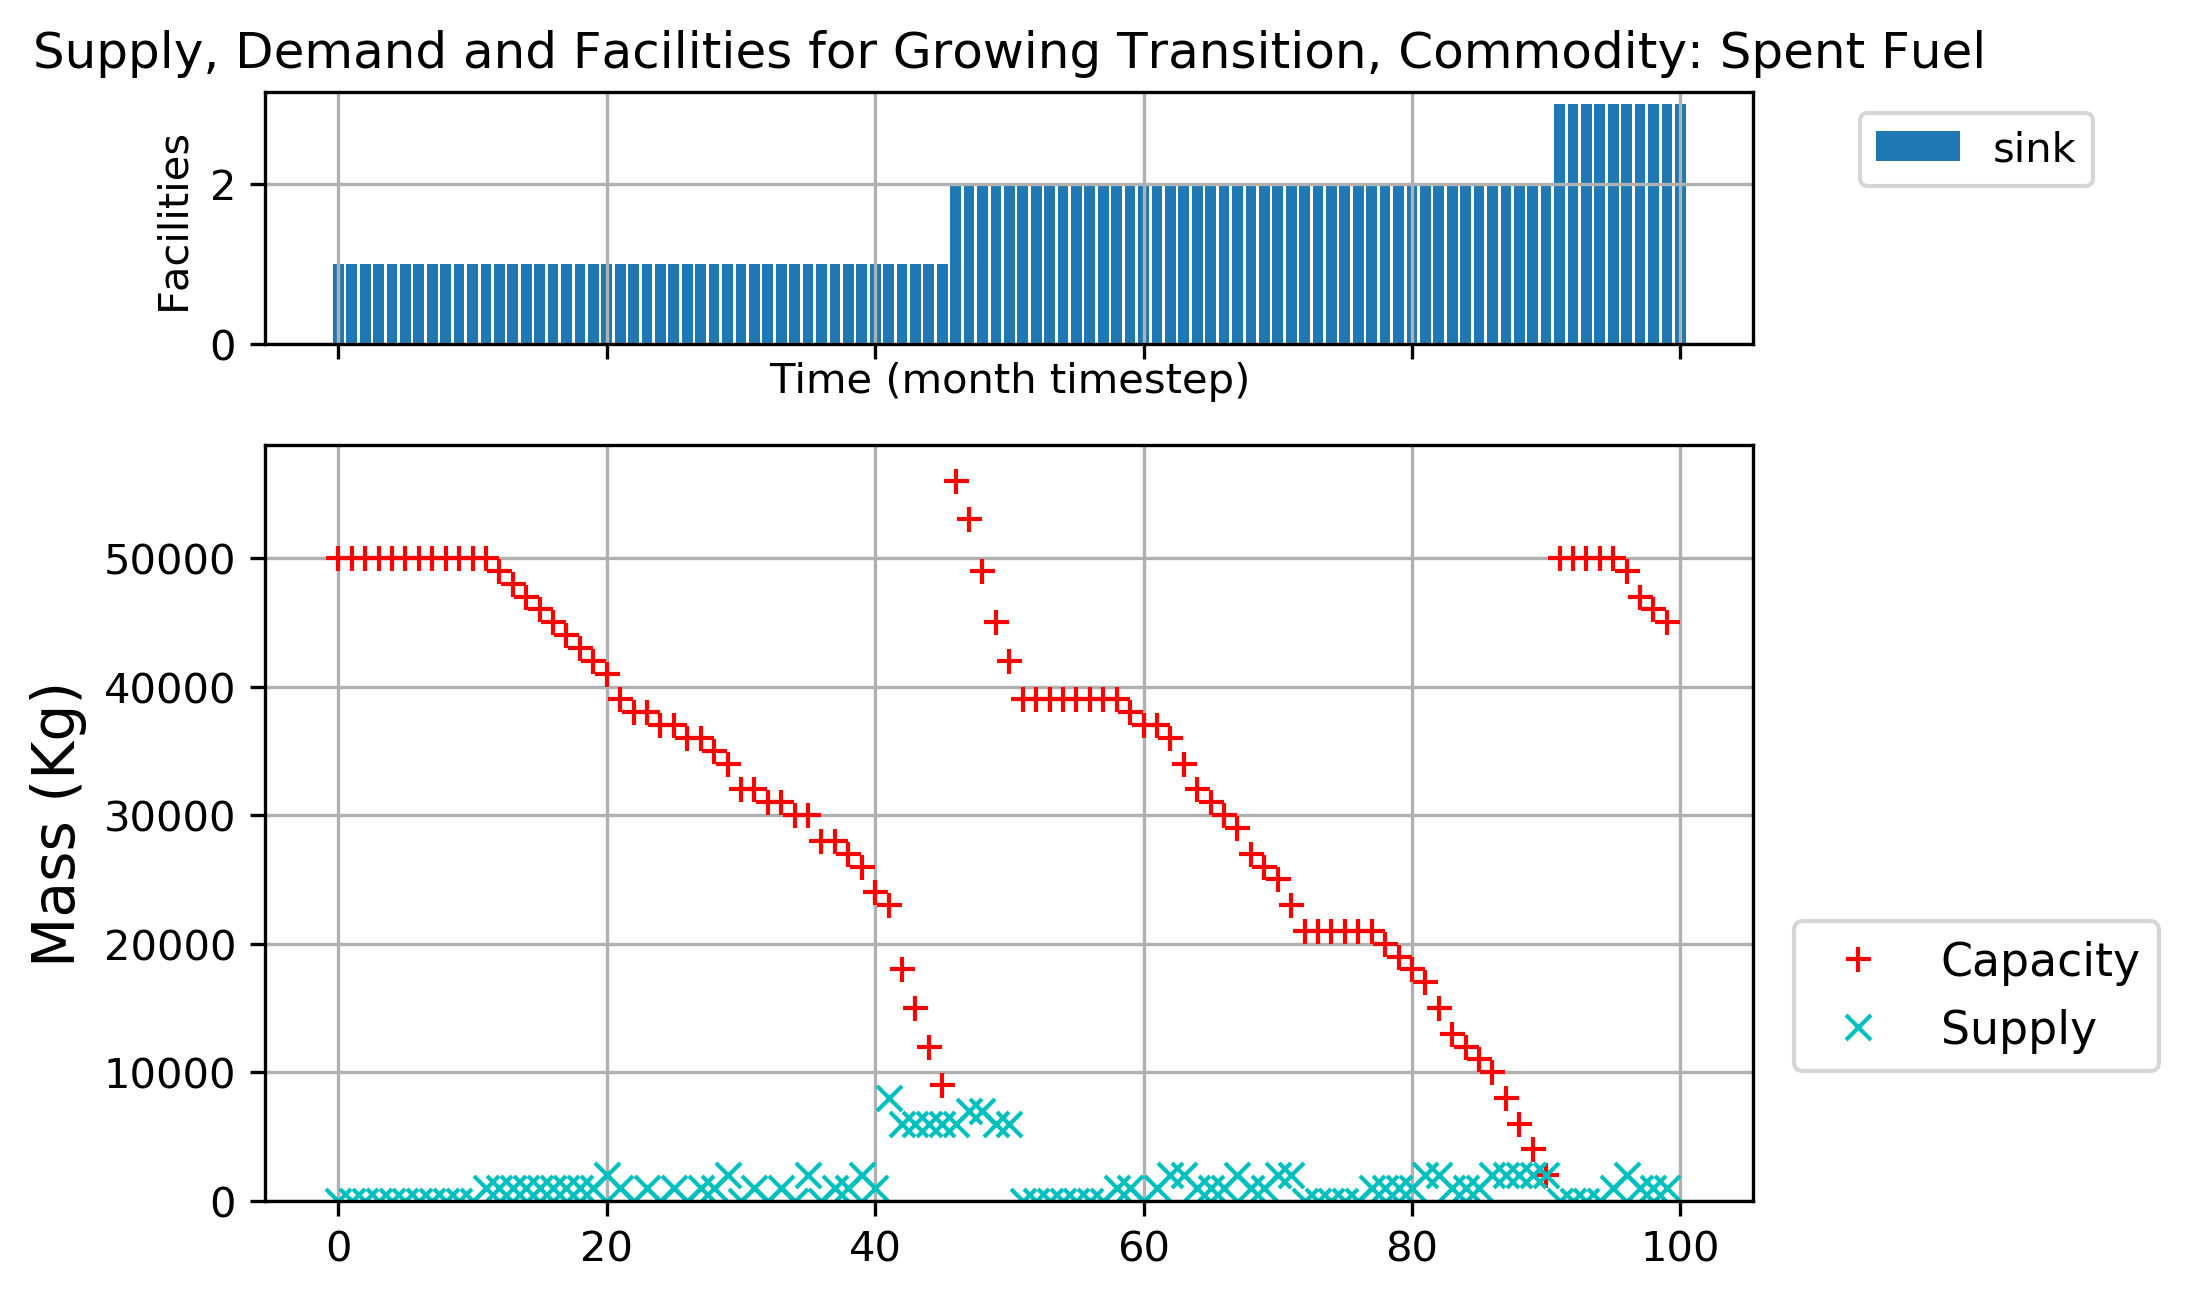
\includegraphics[width=\linewidth]{figures/growingtransition-spentfuel.png} 
            \caption{Spent Fuel is supplied by reactors and the capacity is provided by sink facilities.}
            \label{fig:growingtransition-spentfuel}
        \end{subfigure}
        \caption{Transition Scenario: Linearly increasing power demand.}
    \end{figure}
    
    \subsubsection{\textbf{Basic Transition Scenario Simulation: Sinusoidal Demand}}
    A sinusoidal power demand is the reflection of power demand in 
    the real world where power usage is higher in the winter and summer
    and lower in the spring and fall. 
    Figures \ref{fig:sinetransition-power}, \ref{fig:sinetransition-fuel}
    and \ref{fig:sinetransition-spentfuel} demonstrate the capability 
    of \deploy to deploy reactor and supporting facilities to meet the
    power demand and subsequently demanded secondary commodities 
    for a sinusoidal power demand. 
    Table \ref{tab:transition-scenario-results} shows the number of 
    undersupplied timesteps.
    
    For a sinusoidal power demand, the use of the triple exponential method
    for predicting demand is more effective than the 
    fast fourier transform method which was used for the constant 
    and linearly increasing power demand transition scenarios. 
    This is because the triple exponential smoothing method excels in
    forecasting data points for repetitive seasonal series of data. 
    
    \begin{figure}[]
        \centering
        \begin{subfigure}[t]{\textwidth}
        \centering
            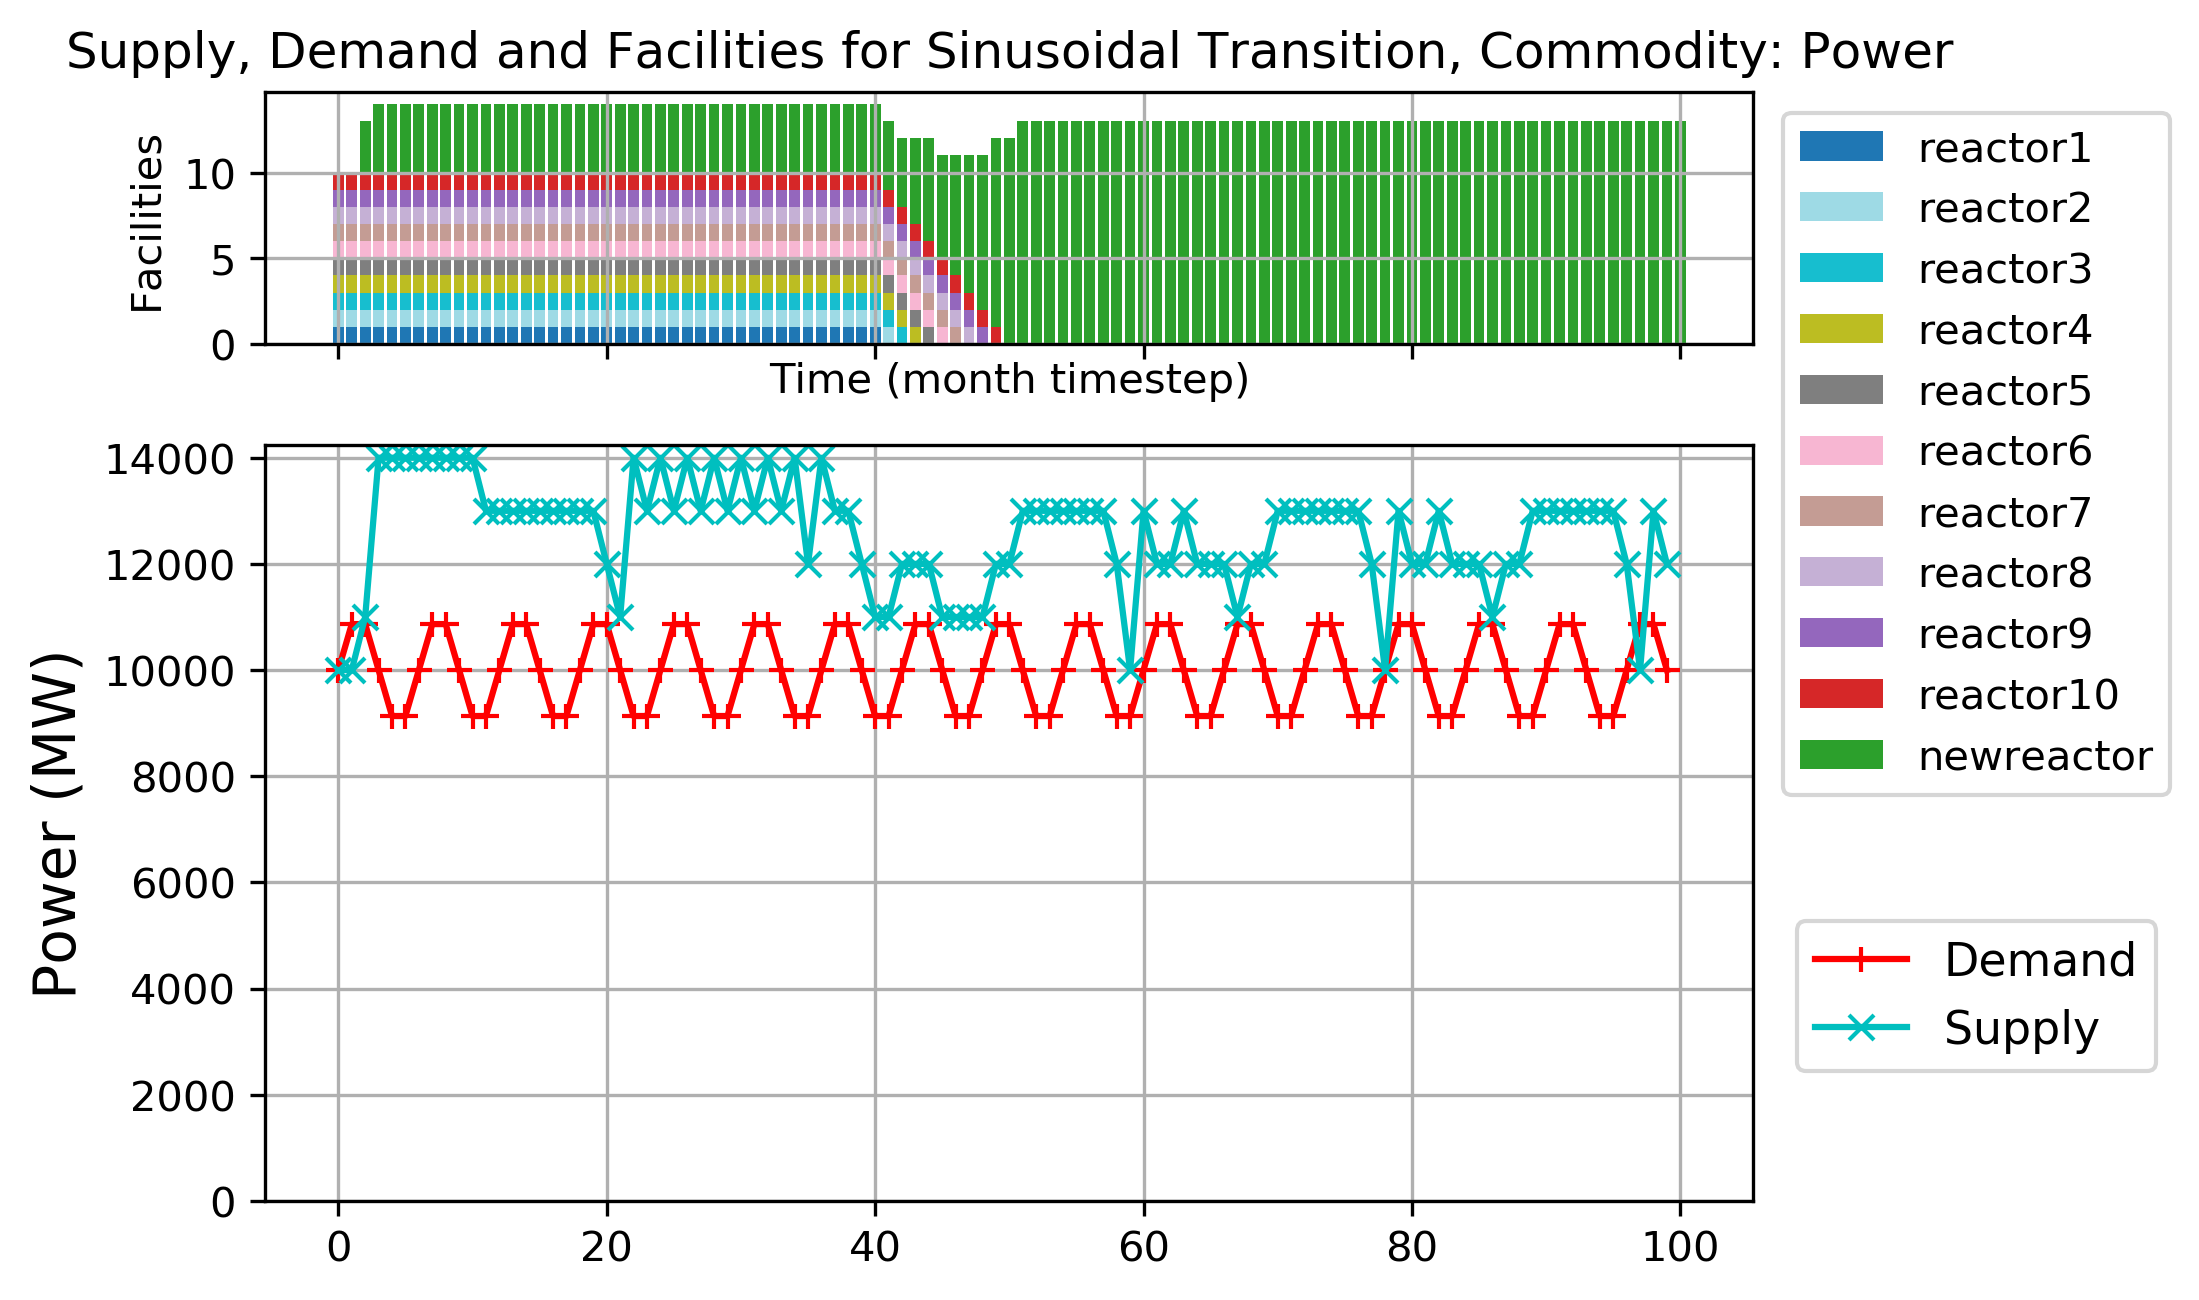
\includegraphics[width=0.7\linewidth]{figures/sinetransition-power.png} 
            \caption{The power demand is a user-defined equation and power is supplied by the reactors.}
            \label{fig:sinetransition-power}
        \end{subfigure}
        \begin{subfigure}[t]{0.6\textwidth}
            \centering
            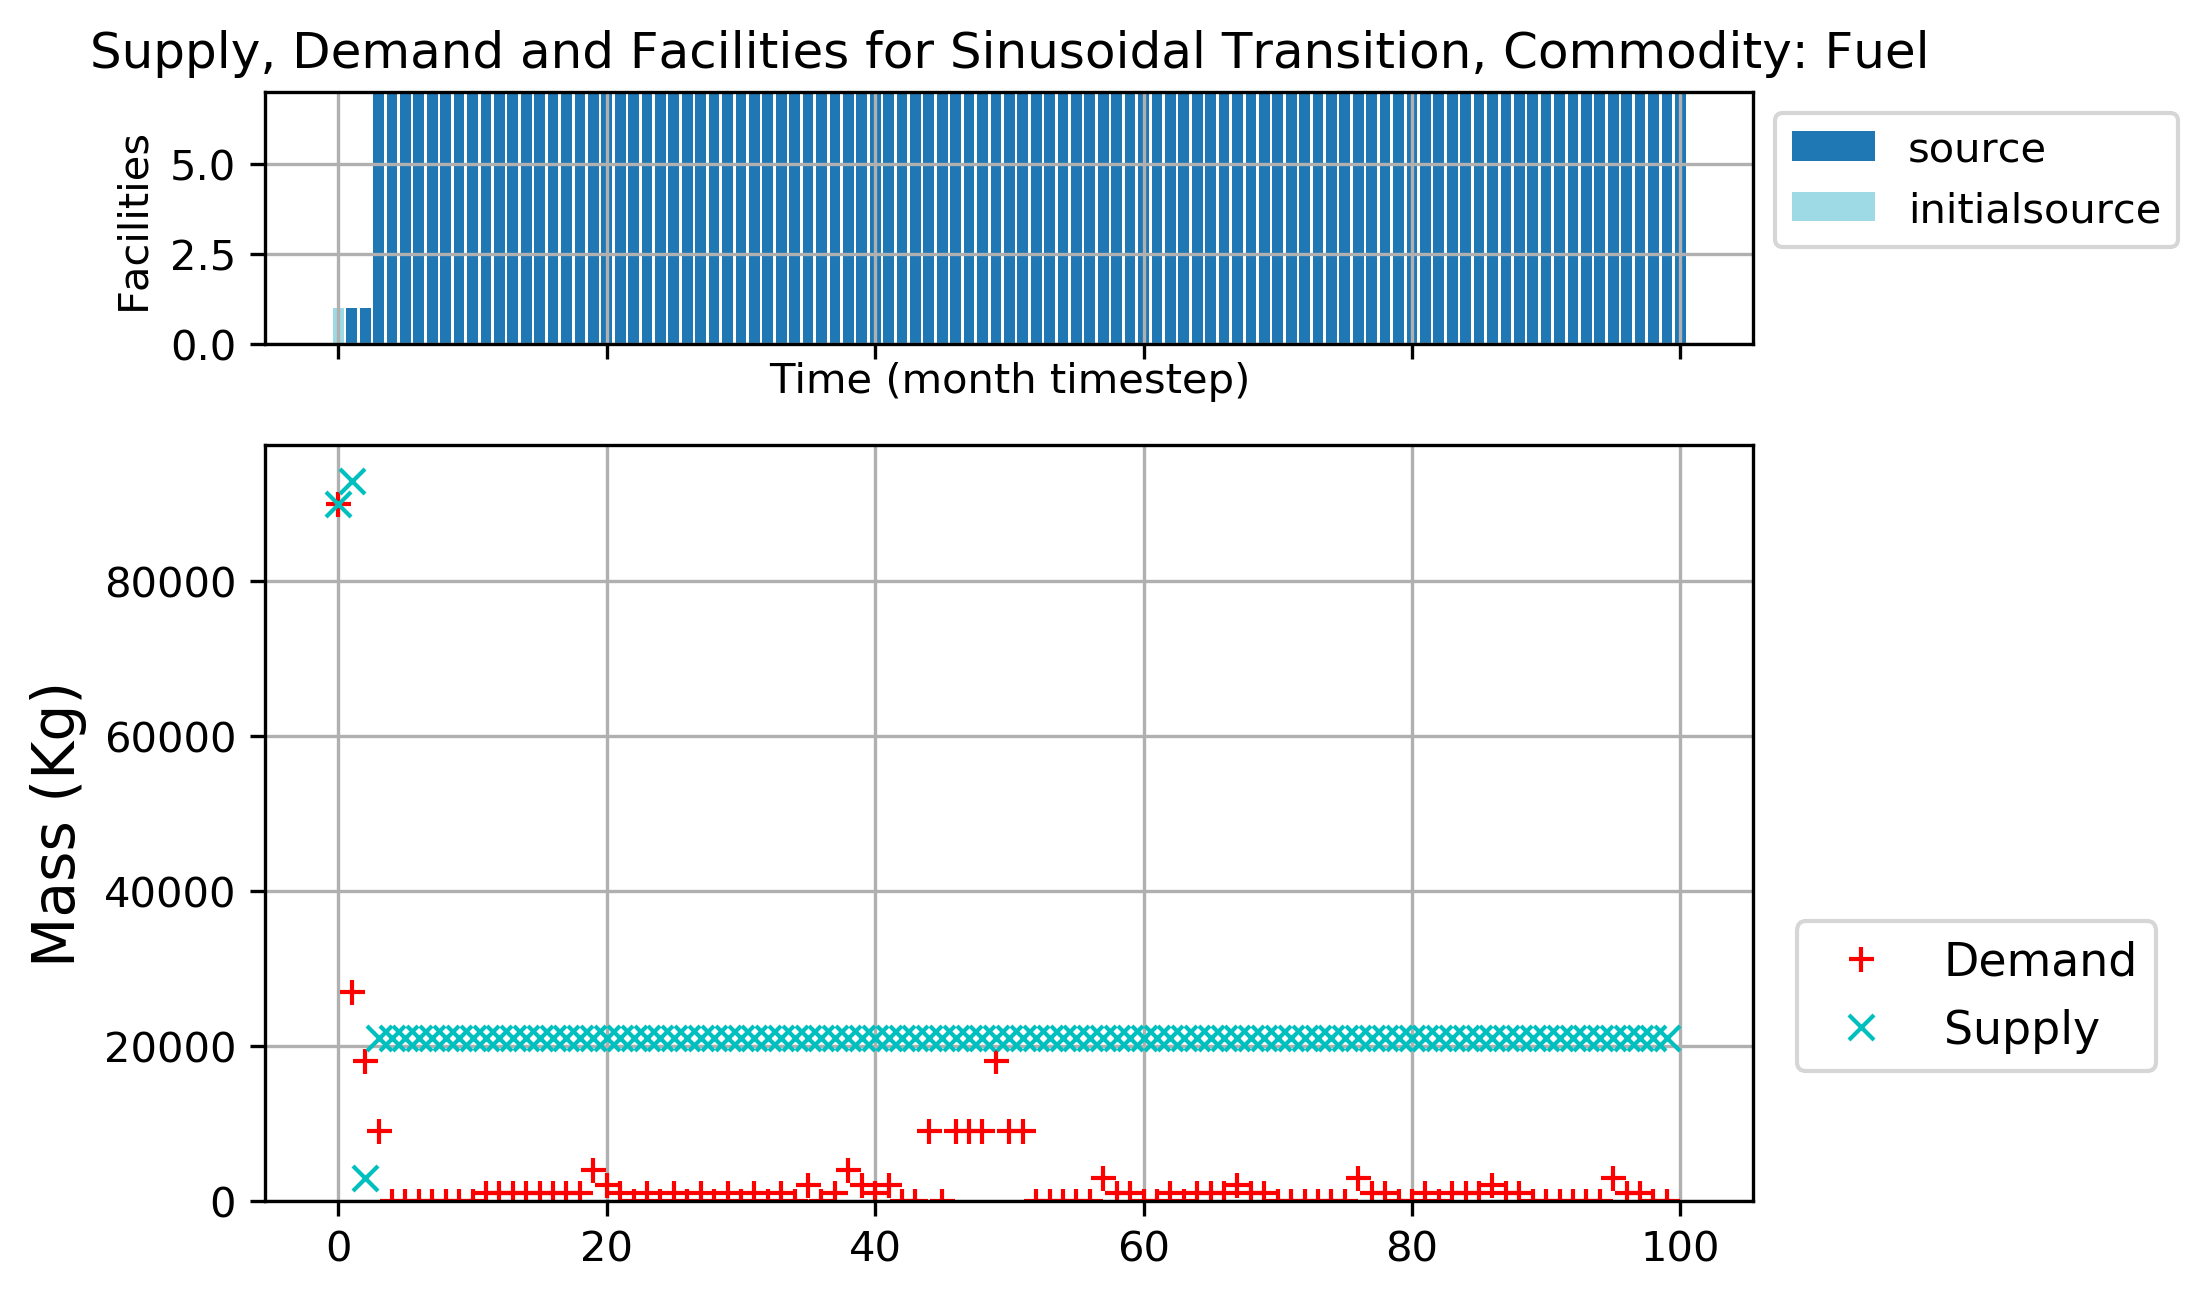
\includegraphics[width=\linewidth]{figures/sinetransition-fuel.png} 
            \caption{Fuel is demanded by reactors and supplied by source facilities.}
            \label{fig:sinetransition-fuel}
        \end{subfigure}
        \begin{subfigure}[t]{0.6\textwidth}
            \centering
            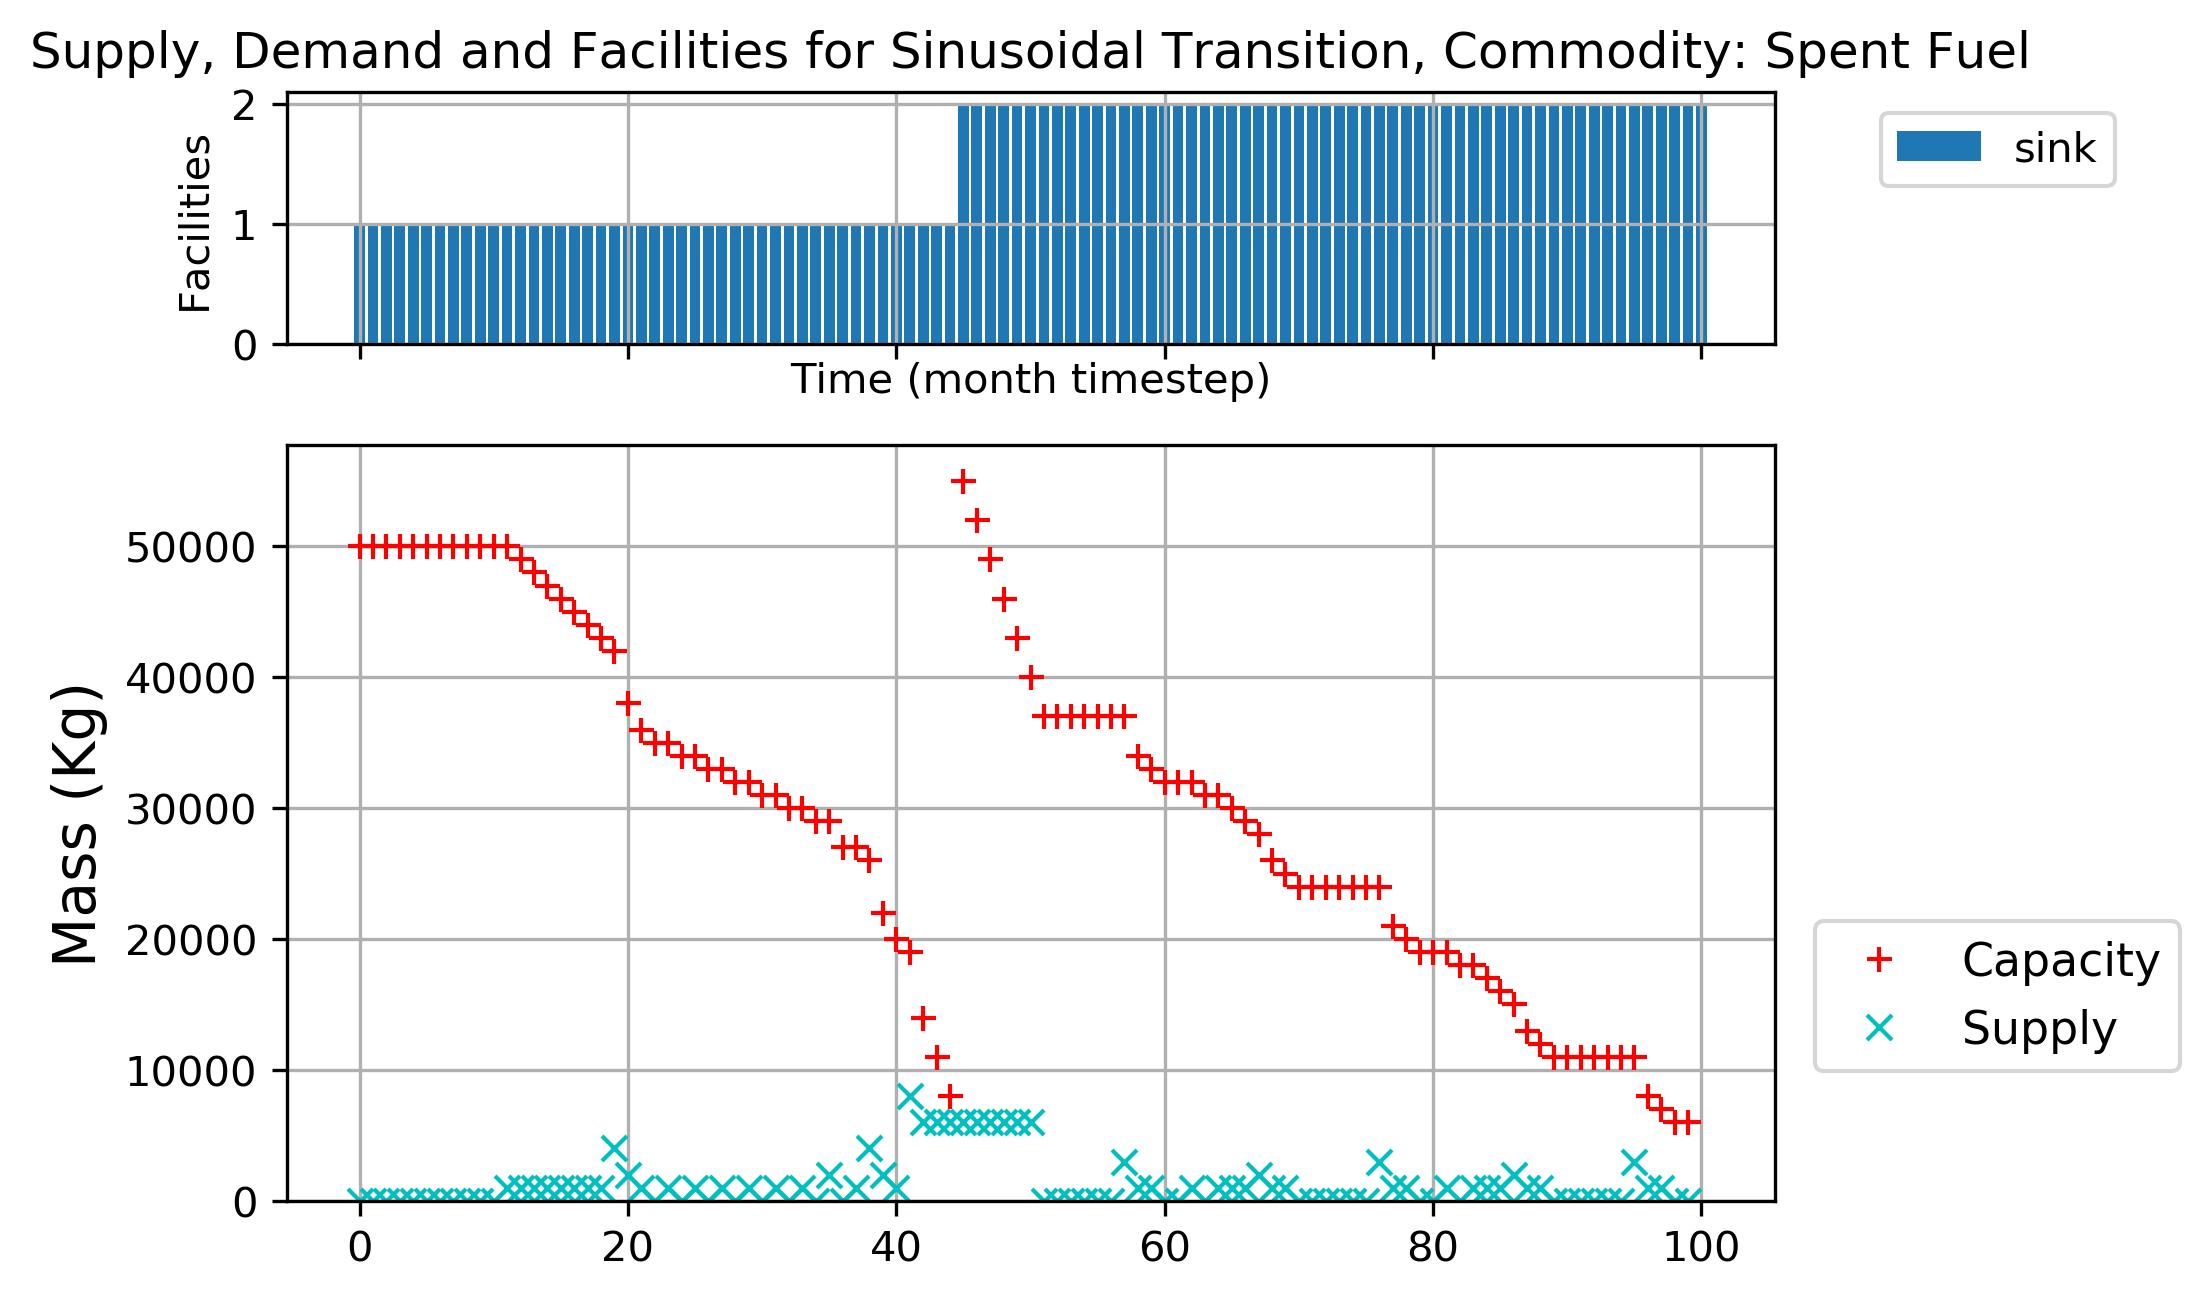
\includegraphics[width=\linewidth]{figures/sinetransition-spentfuel.png} 
            \caption{Spent Fuel is supplied by reactors and the capacity is provided by sink facilities.}
            \label{fig:sinetransition-spentfuel}
        \end{subfigure}
        \caption{Transition Scenario: Sinusoidal Power Demand}
    \end{figure}
    
    \begin{table}[]
        \centering
        \caption {Undersupply results for each commodity in each scenario}
        \label{tab:transition-scenario-results}
        \begin{tabular}{|l|l|p{4cm}|}
        \hline
        \textbf{Basic Transition Scenario}    & \textbf{Commodity}    & \textbf{No. of timesteps with undersupply} \\ \hline
        \multirow{2}{*}{\textbf{Constant Power}} & Fuel & 1 \\ \cline{2-3}
                                                 & Power & 0 \\ \cline{2-3}
                                                 & Spent Fuel & 0 \\ \hline
        \multirow{2}{*}{\textbf{Linearly Increasing Power}} & Fuel & 1 \\ \cline{2-3}
                                                 & Power & 0 \\ \cline{2-3}
                                                 & Spent Fuel & 0 \\ \hline
        \multirow{2}{*}{\textbf{Sinusoidal Power}} & Fuel & 1 \\ \cline{2-3}
                                                 & Power & 1 \\ \cline{2-3}
                                                 & Spent Fuel & 0 \\ \hline
        \end{tabular}
    \end{table}

\section{DYMOND}
DYMOND \cite{yacout_modeling_2005} is a \gls{NFCSim} run within 
the AnyLogic software with Microsoft Excel templates for 
data input and output. 
The major inputs to this code are reactor and fuel cycle 
characteristics, and time-dependent power demand 
\cite{feng_standardized_2016}.   
The code calls ORIGEN \cite{bell_origen_1973} during the simulation 
to conduct reactor depletion calculations. 
The mass flows and inventories are recorded at a system-level
and individual isotopes are tracked. 
DYMOND's main design objective is ease of understanding it's 
behavior and variables. 

In DYMOND, reactor facilities are automatically deployed to 
meet a user-defined power demand and the user can define 
the targeted shares of energy for up to five reactor types. 
The user also defines the fuel loading model used to calculate 
reactor spent fuel compositions, the type of reprocessing 
technology that is used for each reactor type, and the length 
of used fuel cooling time etc. 
In DYMOND, the user must define the deployment schedule for 
the reprocessing plants and the cooling pools and storage pools 
are all assumed to have infinite capacities. 
DYMOND does not have demand-driven deployment capabilities for 
supporting fuel cycle facilities. 

The difference between \Cyclus and DYMOND is that \Cyclus uses 
agent-based modeling for all facilities and mass flows, 
whereas DYMOND uses fleet-based modeling for all facilities and 
mass flows with exception of reactor facilities. 
\Cyclus has the advantage of flexibility and customization, 
and DYMOND has the advantage of ease of use. 

\section{Sensitivity Analysis Capabilities}
In this work, \Cyclus and DYMOND were coupled with Dakota 
\cite{eldred_dakota_2010} to give the \glspl{NFCSim} \gls{SA}, 
\gls{UQ}, and optimization capabilities. 
\chapter{Results}
This chapter will give results on the sensitivity of various 
input parameters of a \gls{NFC} transition scenario. 
Various types of \gls{SA} are conducted. 
The sensitivity analysis was conducted using the Dakota-\Cyclus
and Dakota-Dymond coupling. 
This chapter is broken into five main sections: 
\begin{enumerate}
    \item Sensitivity Analysis Evaluation Criteria 
    \item Transition Scenario Specification 
    \item One-at-a-time \gls{SA} results 
    \item Synergistic \gls{SA} results
    \item Global \gls{SA} results 
\end{enumerate}


\section{Sensitivity Analysis Evaluation Criteria}
Table \ref{tab:category-output-DD} shows which output variables 
the evaluation criteria are associated with. 

\begin{table}[]
    \centering
	\caption {Evaluation criteria and their associated output variables for Dymond-Dakota sensitivity analysis.}
	\label{tab:category-output-DD}
        \footnotesize
        \begin{tabularx}{\textwidth}{l|LL}	
            	\hline
            \textbf{Evaluation Metrics} & \textbf{Output Variable} & \textbf{Indicators}\\
            \hline
            \textbf{Waste Management} & \begin{tabular}[c]{@{}l@{}}Total \gls{HLW} Inventory\\ Depleted Uranium\end{tabular} & \begin{tabular}[c]{@{}l@{}}Final \& Transition Final\\ Final \& Transition Final\end{tabular}\\
            \hline
            \textbf{Proliferation Risk} &  \begin{tabular}[c]{@{}l@{}}Pu in cooling pools\\ Separated Pu in storage \\ Separated Pu in HLW \\Fissile Pu in cooling pools \\ 
            Fissile Separated Pu in storage \\ Fissile Separated Pu in HLW \\\end{tabular} & 
            \begin{tabular}[c]{@{}l@{}} Max, Year, Quality, Slope\\ Max, Year, Quality, Slope \\ Max, Year, Quality, Slope \\ Max, Year, Slope \\ Max, Year, Slope \\ Max, Year, Slope\end{tabular} \\
            
            \hline
            \textbf{Resource Utilization} & Uranium ore consumed & Sum, Transition Sum\\
            \hline
            \textbf{Goodness of Transition} & \begin{tabular}[c]{@{}l@{}}Total Idle Capacity\\ Date of Idle Capacity \\ Length of transition\end{tabular} & \begin{tabular}[c]{@{}l@{}}Sum \\ Final \\ -\end{tabular} \\ 
            \hline
            \end{tabularx}
\end{table}

To quantify the impact of the variation of an input parameter 
on an output parameter, it is necessary to define output indicators 
to measure this impact \cite{noauthor_effects_2017}. 
Output indicators are introduced because the output variables
are a time series resulting in a need for a single value that 
is representative of the output parameter's time series.  
Five types of output indicators are introduced 
\cite{noauthor_effects_2017}: 
(1) final value at end of simulation
(2) maximum value during simulation, 
(3) minimum value during simulation, 
(4) cumulative sum over the whole simulation, and 
(5) slope of the final 50 points of the simulation.
Depending on the nature of the output parameter, a different 
output indicator will be used. 
The slope indicator determines if a variable is increasing or 
decreasing at the end of the simulation. 
Indicators with transition refer to the indicator value during the 
transition period. 
The transition period is defined as from the year when the first 
transition reactor is built till the year of last idle capacity. 

\subsection{Transition Scenario Specification}

\subsection{One-at-a-time Sensitivity Analysis}

\subsection{Synergistic Sensitivity Analysis}

\subsection{Global Sensitivity Analysis}
\chapter{Results: Sensitivity Analysis}
In this chapter, DYMOND and \Cyclus are used to conduct 
sensitivity analysis studies of the 
EG01-30 \gls{NFC} transition scenario. 
Dakota-\Cyclus (\texttt{dcwrapper}) 
and Dakota-DYMOND coupling (\texttt{ddwrapper})
perform  
one-at-a-time sensitivity analysis (SA), synergistic 
SA, and global SA. 
This chapter has six sections: 
\begin{enumerate}
    \item Transition Scenario Specifications 
    \item Sensitivity Analysis Evaluation Metrics 
    \item One-at-a-time \gls{SA}
    \item Synergistic \gls{SA}
    \item Global \gls{SA}
    \item Main Takeaways 
\end{enumerate}

\section{Transition Scenario Specification}
% improve this section 
Both DYMOND and \Cyclus sensitivity analyses 
use the EG01-30 transition scenario.
Slight differences lie in the values of some input variables. 

\subsection{DYMOND}
The specifications of the EG01-30 transition scenario used in the 
DYMOND sensitivity analysis
are described in the DYMOND OECD benchmark transition 
scenario presented at the 17th Meeting of Expert Group on Advanced 
Fuel Cycle Scenarios in France in 2017 
\cite{oecd_nuclear_energy_agency_wpfc_nodate}. 
The OECD benchmark scenario is based on the EG01-30 transition scenario 
in which a \gls{PWR} fleet is transitioned to
a mixed fleet of \gls{MOX} \glspl{PWR} and \glspl{SFR}. 
Table \ref{tab:dymondinputs} describe high-level OECD benchmark transition 
scenario specifications. 

\begin{table}[H]
    \centering
    \doublespacing
    \caption{OECD Benchmark Transition Scenario
	Specifications \cite{oecd_nuclear_energy_agency_wpfc_nodate}}
	\label{tab:dymondinputs}
    \small
    \begin{tabular}{ll}
    \hline
                               \textbf{Input Parameter}            & \textbf{Value}            \\ \hline
    Demand driving commodity   & Power              \\
                               Demand equation {[}TWhe/y{]}   & 430        \\
                               Transition Start Date [Year] & 80\\ 
                               Fleet share ratio [\%] & \gls{MOX} \gls{PWR}: 15\%, \gls{SFR}: 85\%\\ \hline
    \end{tabular}%
    \end{table}

\subsection{\Cyclus}
\Cyclus transition scenario sensitivity analysis uses 
the linearly increasing power demand EG01-30 transition scenario 
(described in Section \ref{sec:eg01-30}).  
Figure \ref{fig:30flow} shows the facility and mass flow 
for this transition scenario in \Cyclus. 
Tables \ref{tab:bestinputs} and \ref{tab:facinputs}
shows the input parameters for \deploy and facilities
in the transition scenario. 
The \texttt{reactor} facility used in the \Cyclus simulation 
is a recipe reactor; it accepts a fresh fuel recipe and outputs 
a spent fuel recipe. 
The recipes used for the \gls{LWR}, \gls{MOX} \gls{LWR}, and 
\gls{SFR} are based on recipes generated by VISION 
\cite{chee_arfc/transition-scenarios_2018}
that closely match EG30 scenario specifications in 
Appendix B of the \gls{DOE} Evaluation and Screening Study 
(E\&S study) \cite{wigeland_nuclear_2014}. 

\begin{table}[H]
    \centering
    \doublespacing
    \caption{\Cyclus facility input parameters for
	EG01-EG30 transition scenario
	that minimizes undersupply for power and minimizes 
	the undersupply and under capacity for other facilities. }
	\label{tab:facinputs}
    \small
    \begin{tabular}{lll}
        \hline
        \textbf{Facility}                 & \textbf{Input Parameter}                    & \textbf{Value} \\ \hline
        \multirow{4}{*}{\textbf{LWR}}     & Lifetime {[}months{]}              & 960   \\
                                 & Cycle time {[}months{]}            & 18    \\
                                 & Refuel time {[}months{]}           & 1     \\
                                 & Rated Power {[}MWe{]}              & 1000  \\ \hline
        \multirow{2}{*}{\textbf{MOX LWR}} & Lifetime {[}months{]}              & 960   \\
                                 & Cycle time {[}months{]}            & 18    \\
                                 & Refuel time {[}months{]}           & 1     \\
                                 & Rated Power {[}MWe{]}              & 1000  \\ \hline
        \multirow{4}{*}{\textbf{SFR}}     & Lifetime {[}months{]}              & 720   \\
                                 & Cycle time {[}months{]}            & 12    \\
                                 & Refuel time {[}months{]}           & 1     \\
                                 & Rated Power {[}MWe{]}              & 333   \\ \hline
        \textbf{Cooling Pools}            & Used fuel storage time {[}years{]} & 3  \\ \hline
        \end{tabular}
    \end{table}

\section{Sensitivity Analysis: Evaluation Metrics}
Important optimization metrics and their associated output variables 
must be defined to determine the basis of comparison for sensitivity 
analysis of \gls{NFC} transition scenarios.
The E\&S study \cite{wigeland_nuclear_2014} evaluated transition 
scenarios using nine metrics: nuclear waste 
management, proliferation risk, nuclear material security risk, 
safety, environmental impact, resource utilization, development 
and deployment risk, institutional issues, financial risk, and 
economics. 
These nine metrics can be narrowed down into four categories
 \cite{passerini_systematic_2014}: environmental 
impact, economics, proliferation risk and resource utilization. 

It is necessary to define output indicators to measure the 
impact of the variation of an input parameter on an output 
parameter \cite{noauthor_effects_2017}. 
Output indicators are introduced because the output variables
are a time series resulting in a need for a single value that 
is representative of the output parameter's time series.  
Four types of output indicators are introduced 
\cite{noauthor_effects_2017}: 
(1) final value at the end of simulation
(2) maximum value during simulation,  
(3) cumulative sum over the whole simulation, and 
(4) quality of Plutonium (equation \ref{eq:pu}). 
A different output indicator is used depending on 
the nature of the output parameter.

\begin{align}
    \label{eq:pu}
Quality\ of\ Pu = \frac{Pu_{239}+Pu_{241}}{Pu_{238}+Pu_{240}+Pu_{242}+Pu_{243}+Pu_{244}}
\end{align}

Table \ref{tab:category-output-DD} shows the four evaluation 
metrics and the associated output variables used in this work. 

\begin{table}[H]
    \centering
    \doublespacing
    \caption {Evaluation metrics and their associated output 
    variables for sensitivity analysis.}
	\label{tab:category-output-DD}
        \small
        \begin{tabular}{lll}	
            	\hline
            \textbf{Evaluation Metrics} & \textbf{Output Variable} & \textbf{Indicators}\\
            \hline
            \textbf{Waste Management} & \begin{tabular}[c]{@{}l@{}}Total High Level Waste Inventory\\ Depleted Uranium\end{tabular} & \begin{tabular}[c]{@{}l@{}}Final \\ Final \end{tabular}\\
            \hline
            \textbf{Proliferation Risk} &  \begin{tabular}[c]{@{}l@{}}Pu in Cooling Pools\\ Separated Pu in Storage \\ Separated Pu in HLW \\ 
            \end{tabular} & 
        \begin{tabular}[c]{@{}l@{}} Max, Quality\\ Max, Quality \\ Max, Quality \end{tabular} \\
            
            \hline
            \textbf{Resource Utilization} & Uranium ore consumed & Sum\\
            \hline
            \textbf{Goodness of Transition} & \begin{tabular}[c]{@{}l@{}}Total Idle Capacity\\ Date of Final Idle Capacity \\ Length of transition\end{tabular} & \begin{tabular}[c]{@{}l@{}}Sum \\ Final \\ -\end{tabular} \\ 
            \hline
            \end{tabular}
\end{table}

The operational conditions for the advanced reactors and
the specifics of the transition scenario are variable
since the fuel cycle simulator is modeling future 
trajectories. 
In the transition scenarios, we vary the following 
input parameters: 
\begin{itemize}
    \item Length of used fuel cooling time 
    \item Fleet share ratio of PWR MOX and SFR reactors 
	\item Introduction date of advanced reactor technology
\end{itemize}

In the following sections, 
we conduct one-at-a-time, synergistic, and global
sensitivity analysis of these three input parameters and 
quantify the evaluation metric impact.  

\section{One-at-a-time Sensitivity Analysis}
\label{sec:oat}

\subsection{Length of cooling time for used fuel}
In the DYMOND and \Cyclus EG01-30 transition scenarios, 
we varied used fuel cooling time from 0 to 8 years. 
These simulations are compared based on the evaluation 
metrics described in Table \ref{tab:category-output-DD}.

\subsubsection{\textbf{DYMOND}}
Tables \ref{tab:dymond-ct-1} and \ref{tab:dymond-ct-2} show 
the absolute values of 
output variables associated with the environmental impact, 
resource utilization, and goodness of transition evaluation 
metrics for each scenario. 
Tables \ref{tab:dymond-ct-sa-1} and \ref{tab:dymond-ct-sa-2} 
show each scenario's percentage 
difference compared with the base case of `Cooling Time = 2 years'
scenario.

In Table \ref{tab:dymond-ct-1}, total idle capacity 
in the simulation increases for used fuel cooling time of 3 years 
onwards. 
This is because the fuel management strategy in the 
DYMOND OECD benchmark scenario was 
manually edited to work best with a 2 year used fuel cooling time.
The idle capacity in cooling time of 3 years onwards could be 
avoided by manually changing the fuel management strategy
in the DYMOND input file for the scenario. 
We did not manually change the fuel management strategy
because this is a one-at-a-time \gls{SA} study 
and, thus, only used fuel cooling time was varied. 

In Table \ref{tab:dymond-ct-sa-2}, compared to the base case, 
as cooling time increases, maximum Pu in the cooling pools increases.
This is expected since there is a larger inventory of used fuel 
in the cooling pools when cooling time increases. 
The quality of Pu in the cooling pools also increases as cooling time 
increases. 
% add more description?  

\begin{table}[H]
    \centering
    \caption{DYMOND: Assessment of how variation of used fuel cooling times
    impacts evaluation metrics (waste management, resource utilization, 
    and goodness of transition) for OECD benchmark transition scenario.}
	\label{tab:dymond-ct-1}
        \scriptsize
        \begin{tabularx}{\textwidth}{R|RR|R|RRR}	
            \hline
            \textbf{} & \multicolumn{2}{c|}{\textbf{Environmental Impact}}                                                                                                                                                                                                                                                      & \textbf{Resource Utilization}                                                                                        & \multicolumn{3}{c}{\textbf{Goodness of Transition}}                                                                                                                                                                                 \\ \hline
\textbf{Scenario: Used Fuel Cooling Time [Year]} & \textbf{Final HLW [kg] } & \textbf{Final Depleted U [kg]} &  \textbf{Total Mined Uranium Ore [kg]}  & \textbf{Total Idle Capacity[kg]} & \textbf{Year of Final Idle Capacity} & \textbf{Length of Transition [years]} \\ \hline
 0  &           1103.2 &                             916933.4 &                       16188.8 &                                    30148.8 &                      301 &                     227 \\ 
 1  &           1101.6 &                             916618.2 &                       16188.8 &                                    30148.8 &                      301 &                     227 \\ 
 2  &           1105.7 &                             916237.60 &                       16188.8 &                                    30148.8 &                      301 &                     227 \\ 
 3  &           1108.3 &                             916268.7 &                       16188.8 &                                   256588.8 &                      301 &                     227 \\ 
 4  &           1099.8 &                             916962.4 &                       16188.8 &                                 1338604.8 &                      301 &                     227 \\ \hline
\end{tabularx}%
\end{table}

\begin{table}[H]
    \centering
    \caption{DYMOND: Assessment of how variation of used fuel cooling times
    impacts evaluation metrics (proliferation risk) for OECD benchmark
	transition scenario.}
	\label{tab:dymond-ct-2}
        \scriptsize
        \begin{tabularx}{\textwidth}{R|RRRRRR}	
            \hline
            \textbf{} & \multicolumn{6}{c}{\textbf{Proliferation Risk}}  \\ \hline
\textbf{Scenario: Used Fuel Cooling Time [Year]} & \textbf{Max Pu in cooling pools [kg] } & \textbf{Pu Quality at max Pu in cooling pools [kg]} &  \textbf{Max Pu in HLW [kg]}  & \textbf{Pu Quality at max Pu in HLW [kg]} & \textbf{Max Pu in Rpr facilities [kg]} & \textbf{Pu Quality at max Pu in Rpr facilities [kg]} \\ \hline
 0  &           0.0 &                             0 &                       18.374 &                                    0.650 &                      208.6 &                     - \\ 
 1  &           105.2 &                             0.652 &                       18.385 &                                    0.652 &                      208.6 &                     - \\ 
 2  &           196.8 &                             0.622 &                       18.409 &                                    0.653 &                      208.6 &                     - \\ 
 3  &           264.8 &                             0.659 &                       18.189 &                                   0.654 &                      208.6 &                     - \\ 
 4  &           348.2 &                             0.671 &                       16.805 &                                 0.658 &                      208.6 &                     - \\ \hline
\end{tabularx}%
\end{table}

\begin{table}[H]
    \caption{DYMOND: Sensitivity analysis of how variation of used fuel 
    cooling times impacts evaluation metrics (waste management, resource utilization, 
    and goodness of transition) for OECD benchmark transition scenario.
    The numbers in the table represent the percentage difference between 
    an output variable from each scenario and the base case scenario (Cooling time = 2 years).}
    \label{tab:dymond-ct-sa-1}
    \scriptsize
    \begin{tabularx}{\textwidth}{R|RR|R|RRR}	
		\hline
        \textbf{} & \multicolumn{2}{c|}{\textbf{Environmental Impact}}                                    & \textbf{Resource Utilization}                                                                                       & \multicolumn{3}{c}{\textbf{Goodness of Transition}}                                                                                                                                                                                 \\ \hline
        \textbf{Scenario: Used Fuel Cooling Time [Year]} & \textbf{Final HLW [\%] } & \textbf{Final Depleted U [\%]} &  \textbf{Total Mined Uranium Ore [\%]]}  & \textbf{Total Idle Capacity [\%]} & \textbf{Year of Final Idle Capacity [\%]} & \textbf{Length of Transition [\%]} \\ \hline
         0  &             \cellcolor[HTML]{67FD9A}-0.221736 &                                   \cellcolor[HTML]{67FD9A}0.075939 &                                                            \cellcolor[HTML]{67FD9A}0.0 &                 \cellcolor[HTML]{67FD9A}0.000000 &                                           \cellcolor[HTML]{67FD9A}0.0 & \cellcolor[HTML]{67FD9A}0.0 \\
		 1  &             \cellcolor[HTML]{67FD9A}-0.363540 &                                    \cellcolor[HTML]{67FD9A}0.041532 &                                                           \cellcolor[HTML]{67FD9A}0.0 &                 \cellcolor[HTML]{67FD9A}0.000000 &                                          \cellcolor[HTML]{67FD9A}0.0 & \cellcolor[HTML]{67FD9A}0.0 \\ 
		 2  &              \cellcolor[HTML]{000000}0.000000 &                                     \cellcolor[HTML]{000000}0.000000 &                                                              \cellcolor[HTML]{000000}0.0 &                 \cellcolor[HTML]{000000}0.000000 &                                         \cellcolor[HTML]{000000}0.0 & \cellcolor[HTML]{000000}0.0 \\ 
		 3  &              \cellcolor[HTML]{67FD9A}0.234524 &                                    \cellcolor[HTML]{67FD9A}0.003389 &                                                              \cellcolor[HTML]{67FD9A}0.0 &               \cellcolor[HTML]{FD6864}751.074670 &                                         \cellcolor[HTML]{67FD9A}0.0 & \cellcolor[HTML]{67FD9A}0.0 \\ 
		 4  &             \cellcolor[HTML]{67FD9A}-0.529033 &                                   \cellcolor[HTML]{67FD9A}0.079102 &                                                        \cellcolor[HTML]{67FD9A}0.0 &              \cellcolor[HTML]{FD6864}4339.993632 &                                        \cellcolor[HTML]{67FD9A}0.0 & \cellcolor[HTML]{67FD9A}0.0 \\ \hline
	\end{tabularx}%
    
    \resizebox{0.3\textwidth}{!}{
    \fbox{\begin{tabular}{ll}
        \textcolor{green}{$\blacksquare$} & $sensitivity \leq 1\%$ \\
        \textcolor{orange}{$\blacksquare$} & $1\% < sensitivity < 10\%$ \\
        \textcolor{red}{$\blacksquare$} & $sensitivity \geq 10\%$
        \end{tabular}}}
    \end{table}

    \begin{table}[H]
        \caption{DYMOND: Sensitivity analysis of how variation of used fuel 
        cooling times impacts evaluation metrics (proliferation risk)for OECD benchmark transition scenario.
        The numbers in the table represent the percentage difference between 
    an output variable from each scenario and the base case scenario (Cooling time = 2 years).}
        \label{tab:dymond-ct-sa-2}
        \scriptsize
        \begin{tabularx}{\textwidth}{R|RRRRRR}	
            \hline
            \textbf{} & \multicolumn{6}{c}{\textbf{Proliferation Risk}}  \\ \hline
\textbf{Scenario: Used Fuel Cooling Time [Year]} & \textbf{Max Pu in cooling pools [\%] } & \textbf{Pu Quality at max Pu in cooling pools [\%]} &  \textbf{Max Pu in HLW [\%]}  & \textbf{Pu Quality at max Pu in HLW [\%]} & \textbf{Max Pu in Rpr facilities [\%]} & \textbf{Pu Quality at max Pu in Rpr facilities [\%]} \\ \hline
             0  &             \cellcolor[HTML]{FD6864}-100 &                                   \cellcolor[HTML]{FD6864}-100 &                                                            \cellcolor[HTML]{67FD9A}-0.19 &                 \cellcolor[HTML]{67FD9A}-0.459 &                                           \cellcolor[HTML]{67FD9A}0.0 & \cellcolor[HTML]{67FD9A}- \\
             1  &             \cellcolor[HTML]{FD6864}-46.5 &                                    \cellcolor[HTML]{FE996B}4.82 &                                                           \cellcolor[HTML]{67FD9A}-0.13 &                 \cellcolor[HTML]{67FD9A}-0.153 &                                          \cellcolor[HTML]{67FD9A}0.0 & \cellcolor[HTML]{67FD9A}- \\ 
             2  &              \cellcolor[HTML]{000000}0.000000 &                                     \cellcolor[HTML]{000000}0.000000 &                                                              \cellcolor[HTML]{000000}0.0 &                 \cellcolor[HTML]{000000}0.000000 &                                         \cellcolor[HTML]{000000}0.0 & \cellcolor[HTML]{000000}0.0 \\ 
             3  &              \cellcolor[HTML]{FD6864}34.5 &                                    \cellcolor[HTML]{FE996B}5.95 &                                                              \cellcolor[HTML]{FE996B}-1.20 &               \cellcolor[HTML]{FD6864}0.153 &                                         \cellcolor[HTML]{67FD9A}0.0 & \cellcolor[HTML]{67FD9A}- \\ 
             4  &             \cellcolor[HTML]{FD6864}76.9 &                                   \cellcolor[HTML]{FE996B}7.88 &                                                        \cellcolor[HTML]{FE996B}-8.71 &              \cellcolor[HTML]{FD6864}0.766 &                                        \cellcolor[HTML]{67FD9A}0.0 & \cellcolor[HTML]{67FD9A}- \\ \hline
        \end{tabularx}%
        
        \resizebox{0.3\textwidth}{!}{
        \fbox{\begin{tabular}{ll}
            \textcolor{green}{$\blacksquare$} & $sensitivity \leq 1\%$ \\
            \textcolor{orange}{$\blacksquare$} & $1\% < sensitivity < 10\%$ \\
            \textcolor{red}{$\blacksquare$} & $sensitivity \geq 10\%$
            \end{tabular}}}
        \end{table}

    
\subsubsection{\textbf{\Cyclus}}

Tables \ref{tab:cyclus-ct-1} and \ref{tab:cyclus-ct-2} show 
the absolute values of 
output variables associated with the environmental impact, 
resource utilization, and goodness of transition evaluation 
metrics for each scenario. 
Tables \ref{tab:cyclus-ct-sa-1} and \ref{tab:cyclus-ct-sa-2} 
show each scenario's percentage 
difference compared with the base case of `Cooling Time = 2 years'
scenario.

In Table \ref{tab:cyclus-ct-sa-1}, most evaluation metrics do not change 
for variation in the used fuel cooling time, with exception of the final 
HLW amount in the scenario. 
Final HLW amount decreases for a longer used fuel cooling time.
In Table \ref{tab:cyclus-ct-sa-2}, compared to the base case, 
as cooling time increases, maximum Pu in the cooling pools increases.
This is similar to the result for the DYMOND transition scenario (table 
\ref{tab:dymond-ct-sa-2}). 
This is expected since there will be a larger inventory of used fuel 
in the cooling pools when cooling time increases. 
The quality of Pu in the cooling pools decreases as cooling time 
increases. 
Maximum Pu in HLW and reprocessing facilities, and their corresponding 
Pu quality, decrease for a longer cooling time. 

\begin{table}[H]
    \centering
    \caption{\Cyclus: Assessment of how variation of used fuel cooling times
    impacts evaluation metrics (waste management, resource utilization, 
    and goodness of transition) for OECD benchmark transition scenario.}
	\label{tab:cyclus-ct-1}
        \scriptsize
        \begin{tabularx}{\textwidth}{R|RR|R|RRR}
            \hline	
            \textbf{} & \multicolumn{2}{c|}{\textbf{Environmental Impact}}                                                                                                                                                                                                                                                      & \textbf{Resource Utilization}                                                                                        & \multicolumn{3}{c}{\textbf{Goodness of Transition}}                                                                                                                                                                                 \\ \hline
\textbf{Scenario: Used Fuel Cooling Time [Year]} & \textbf{Final HLW [kg] } & \textbf{Final Depleted U [kg]} &  \textbf{Total Mined Uranium Ore [kg]}  & \textbf{Total Idle Capacity[kg]} & \textbf{Year of Final Idle Capacity} & \textbf{Length of Transition [years]} \\ \hline

0  & 13223828.1 & 798818620.4      & 1.437e11    & 135.1               & 962                     & 2                      \\
2  & 13073261.2 & 798818620.4      & 1.437e11    & 135.1               & 962                     & 2                      \\
4  & 12906058.3 & 798818620.4      & 1.437e11    & 135.1               & 962                     & 2                      \\
6  & 12795682.5 & 798818620.4      & 1.437e11    & 135.1               & 962                     & 2                      \\
8  & 12726528.6 & 798818620.4      & 1.437e11    & 135.1               & 962                     & 2                     \\ \hline 
        \end{tabularx}
\end{table}

\begin{table}[H]
    \centering
    \caption{\Cyclus: Assessment of how variation of used fuel cooling times
    impacts evaluation metrics (proliferation risk) for OECD benchmark
	transition scenario.}
	\label{tab:cyclus-ct-2}
        \scriptsize
        \begin{tabularx}{\textwidth}{R|RRRRRR}	
            \hline
            \textbf{} & \multicolumn{6}{c}{\textbf{Proliferation Risk}}  \\ \hline
\textbf{Scenario: Used Fuel Cooling Time [Year]} & \textbf{Max Pu in cooling pools [kg] } & \textbf{Pu Quality at max Pu in cooling pools [kg]} &  \textbf{Max Pu in HLW [kg]}  & \textbf{Pu Quality at max Pu in HLW [kg]} & \textbf{Max Pu in Rpr facilities [kg]} & \textbf{Pu Quality at max Pu in Rpr facilities [kg]} \\ \hline
0  & 48979.28         & 0.66                           & 44426.65      & 0.62                        & 2800580.69        & 0.49                            \\
2  & 199036.06        & 0.6                            & 43629.18      & 0.62                        & 2637125.07        & 0.48                            \\
4  & 368405.04        & 0.58                           & 42844.4       & 0.62                        & 2460403.99        & 0.48                            \\
6  & 554321.66        & 0.57                           & 42646.72      & 0.62                        & 2290857.92        & 0.47                            \\
8  & 733483.85        & 0.56                           & 42858.1       & 0.62                        & 2111786.28        & 0.47                           \\ \hline
\end{tabularx}%
\end{table}

% add color 
\begin{table}[H]
    \caption{\Cyclus: Sensitivity analysis of how variation of used fuel 
    cooling times impacts evaluation metrics (environmental impact, resource
    utilization, and goodness of transition) for OECD benchmark 
    transition scenario.
    The numbers in the table represent the percentage difference between 
    an output variable from each scenario and the base case scenario (Cooling time = 2 years).}
    \label{tab:cyclus-ct-sa-1}
    \scriptsize
    \begin{tabularx}{\textwidth}{R|RR|R|RRR}	
		\hline
        \textbf{} & \multicolumn{2}{c|}{\textbf{Environmental Impact}}                                    & \textbf{Resource Utilization}                                                                                       & \multicolumn{3}{c}{\textbf{Goodness of Transition}}                                                                                                                                                                                 \\ \hline
        \textbf{Scenario: Used Fuel Cooling Time [Year]} & \textbf{Final HLW [\%] } & \textbf{Final Depleted U [\%]} &  \textbf{Total Mined Uranium Ore [\%]]}  & \textbf{Total Idle Capacity [\%]} & \textbf{Year of Final Idle Capacity [\%]} & \textbf{Length of Transition [\%]} \\ \hline0  & \cellcolor[HTML]{FE996B}1.15      & \cellcolor[HTML]{67FD9A}0.0              & \cellcolor[HTML]{67FD9A}0.0               & \cellcolor[HTML]{67FD9A}0.0                 & \cellcolor[HTML]{67FD9A}0.0                     & \cellcolor[HTML]{67FD9A}0.0                    \\
        2  & \cellcolor[HTML]{000000}0.0       & \cellcolor[HTML]{000000}0.0              & \cellcolor[HTML]{000000}0.0               & \cellcolor[HTML]{000000}0.0                 & \cellcolor[HTML]{000000}0.0                     & \cellcolor[HTML]{000000}0.0                    \\
        4  & \cellcolor[HTML]{FE996B}-1.28       & \cellcolor[HTML]{67FD9A}0.0              & \cellcolor[HTML]{67FD9A}0.0               & \cellcolor[HTML]{67FD9A}0.0                 & \cellcolor[HTML]{67FD9A}0.0                     & \cellcolor[HTML]{67FD9A}0.0                    \\
        6  & \cellcolor[HTML]{FE996B}-2.12     & \cellcolor[HTML]{67FD9A}0.0              & \cellcolor[HTML]{67FD9A}0.0               & \cellcolor[HTML]{67FD9A}0.0                 & \cellcolor[HTML]{67FD9A}0.0                     & \cellcolor[HTML]{67FD9A}0.0                    \\
        8  & \cellcolor[HTML]{FE996B}-2.65     & \cellcolor[HTML]{67FD9A}0.0              & \cellcolor[HTML]{67FD9A}0.0               & \cellcolor[HTML]{67FD9A}0.0                 & \cellcolor[HTML]{67FD9A}0.0                     & \cellcolor[HTML]{67FD9A}0.0                   \\ \hline 
                \end{tabularx}%
    
    \resizebox{0.3\textwidth}{!}{
    \fbox{\begin{tabular}{ll}
        \textcolor{green}{$\blacksquare$} & $sensitivity \leq 1\%$ \\
        \textcolor{orange}{$\blacksquare$} & $1\% < sensitivity < 10\%$ \\
        \textcolor{red}{$\blacksquare$} & $sensitivity \geq 10\%$
        \end{tabular}}}
    \end{table}

    \begin{table}[H]
        \caption{\Cyclus: Sensitivity analysis of how variation of used fuel 
        cooling times impacts evaluation metrics (proliferation risk) for OECD benchmark transition scenario.
        The numbers in the table represent the percentage difference between 
        an output variable from each scenario and the base case scenario (Cooling time = 2 years).}
        \label{tab:cyclus-ct-sa-2}
        \scriptsize
        \begin{tabularx}{\textwidth}{R|RRRRRR}	
            \hline
            \textbf{} & \multicolumn{6}{c}{\textbf{Proliferation Risk}}  \\ \hline
            \textbf{Scenario: Used Fuel Cooling Time [Year]} & \textbf{Max Pu in cooling pools [\%] } & \textbf{Pu Quality at max Pu in cooling pools [\%]} &  \textbf{Max Pu in HLW [\%]}  & \textbf{Pu Quality at max Pu in HLW [\%]} & \textbf{Max Pu in Rpr facilities [\%]} & \textbf{Pu Quality at max Pu in Rpr facilities [\%]} \\ \hline
            0  & \cellcolor[HTML]{FD6864}-75.39           & \cellcolor[HTML]{FE996B}8.99                           & \cellcolor[HTML]{FE996B}1.83          & \cellcolor[HTML]{67FD9A}0.08                        & \cellcolor[HTML]{FE996B}6.2               & \cellcolor[HTML]{FE996B}1.45                            \\
2  &\cellcolor[HTML]{000000}0.0              & \cellcolor[HTML]{000000}0.0                            & \cellcolor[HTML]{000000}0.0           & \cellcolor[HTML]{000000}0.0                         & \cellcolor[HTML]{000000}0.0               & \cellcolor[HTML]{000000}0.0                             \\
4  & \cellcolor[HTML]{FD6864}85.09            & \cellcolor[HTML]{FE996B}-3.34                          & \cellcolor[HTML]{FE996B}-1.8          & \cellcolor[HTML]{67FD9A}-0.12                       & \cellcolor[HTML]{FE996B}-6.7              & \cellcolor[HTML]{FE996B}-1.06                           \\
6  & \cellcolor[HTML]{FD6864}178.5            & \cellcolor[HTML]{FE996B}-5.55                          & \cellcolor[HTML]{FE996B}-2.25         & \cellcolor[HTML]{67FD9A}-0.15                       & \cellcolor[HTML]{FD6864}-13.13            & \cellcolor[HTML]{FE996B}-2.11                           \\
8  & \cellcolor[HTML]{FD6864}268.52           & \cellcolor[HTML]{FE996B}-7.23                          & \cellcolor[HTML]{FE996B}-1.77         & \cellcolor[HTML]{67FD9A}-0.22                       & \cellcolor[HTML]{FD6864}-19.92            & \cellcolor[HTML]{FE996B}-3.0                           \\ \hline
        \end{tabularx}
        \end{table}

\subsection{Fleet share ratio of PWR MOX and SFR reactors}

The fleet share ratio of \gls{MOX} \glspl{PWR} and \glspl{SFR}
was varied from 0\% to 20\% of \gls{MOX} \glspl{PWR} for the 
\Cyclus EG01-30 transition scenario. 
These simulations are compared based on the evaluation 
metrics described in Table \ref{tab:category-output-DD}. 

Tables \ref{tab:cyclus-fs-1} and \ref{tab:cyclus-fs-2} show 
the absolute values of 
output variables associated with the environmental impact, 
resource utilization, and goodness of transition evaluation 
metrics for each scenario. 
Tables \ref{tab:cyclus-fs-sa-1} and \ref{tab:cyclus-fs-sa-2} 
show each scenario's percentage 
difference compared with the base case of `Fleet share = 15\% 
\gls{MOX} \glspl{PWR}' scenario. 

In Table \ref{tab:cyclus-fs-sa-1}, most evaluation metrics do not change 
for variation in fleet share ratio, except for the final 
amount of HLW in the scenario. 
The final amount of HLW is largest for 0\% fleet share of \gls{MOX} 
\glspl{PWR} and decreases as the fleet share of \gls{MOX} \glspl{PWR} 
increases. 
In Table \ref{tab:cyclus-fs-sa-2}, maximum Pu in cooling pools and 
reprocessing facility 
decreases for increasing fleet share ratio of \gls{MOX} \glspl{PWR}; 
however, the quality of Pu increases. 
Maximum Pu in HLW increases for a decreasing fleet share ratio
of \gls{MOX} \glspl{PWR}, while the quality of Pu decreases slightly.
Therefore, if minimizing proliferation risk is a high priority, 
a transition scenario 
with a smaller fleet share of \gls{MOX} \glspl{PWR} is recommended
to minimize the Pu amount in the cooling pools and reprocessing facilities. 

% correct stuff 
\begin{table}[H]
    \centering
    \caption{\Cyclus: Assessment of how variation of fleet share ratio
    of PWR MOX and SFR reactors
    impacts evaluation metrics (environmental impact, resource
    utilization, and goodness of transition) for EG01-30 transition scenario.}
	\label{tab:cyclus-fs-1}
        \scriptsize
        \begin{tabularx}{\textwidth}{R|RR|R|RRR}
            \hline	
            \textbf{} & \multicolumn{2}{c|}{\textbf{Environmental Impact}}                                                                                                                                                                                                                                                      & \textbf{Resource Utilization}                                                                                        & \multicolumn{3}{c}{\textbf{Goodness of Transition}}                                                                                                                                                                                 \\ \hline
\textbf{Scenario: PWR MOX Fleet Share [\%]} & \textbf{Final HLW [kg] } & \textbf{Final Depleted U [kg]} &  \textbf{Total Mined Uranium Ore [kg]}  & \textbf{Total Idle Capacity[kg]} & \textbf{Year of Final Idle Capacity} & \textbf{Length of Transition [years]} \\ \hline

0  & 13153061.6 & 798818620.4      & 1.437e11    & 135.1               & 962                     & 2                      \\
5  & 13056988.7 & 798818620.4      & 1.437e11    & 135.1               & 962                     & 2                      \\
10 & 13051896.3 & 798818620.4      & 1.437e11    & 135.1               & 962                     & 2                      \\
15 & 12959554.1 & 798818620.4      & 1.437e11    & 135.1               & 962                     & 2                      \\
20 & 13002120.9 & 798818620.4      & 1.437e11    & 135.1               & 962                     & 2                     \\ \hline
        \end{tabularx}
\end{table}

% correct stuff 
\begin{table}[H]
    \centering
    \caption{\Cyclus: Assessment of how variation of fleet share ratio
    of PWR MOX and SFR reactors
    impacts evaluation metrics (proliferation risk) for EG01-30 transition scenario.}
	\label{tab:cyclus-fs-2}
        \scriptsize
        \begin{tabularx}{\textwidth}{R|RRRRRR}	
            \hline
            \textbf{} & \multicolumn{6}{c}{\textbf{Proliferation Risk}}  \\ \hline
\textbf{Scenario: PWR MOX Fleet Share [\%]} & \textbf{Max Pu in cooling pools [kg] } & \textbf{Pu Quality at max Pu in cooling pools [kg]} &  \textbf{Max Pu in HLW [kg]}  & \textbf{Pu Quality at max Pu in HLW [kg]} & \textbf{Max Pu in Rpr facilities [kg]} & \textbf{Pu Quality at max Pu in Rpr facilities [kg]} \\ \hline
0  & 256794.03        & 0.66                           & 45816.02      & 0.62                        & 2357604.01        & 0.55                            \\
5  & 273733.13        & 0.62                           & 44338.72      & 0.62                        & 2461421.31        & 0.51                            \\
10 & 279694.78        & 0.61                           & 44055.54      & 0.62                        & 2513133.76        & 0.5                             \\
15 & 285794.85        & 0.59                           & 42905.59      & 0.62                        & 2552142.82        & 0.48                            \\
20 & 291786.54        & 0.58                           & 43133.61      & 0.62                        & 2605589.02        & 0.47                           \\ \hline
\end{tabularx}%
\end{table}

% correct stuff 
\begin{table}[H]
    \caption{\Cyclus: Sensitivity analysis of how variation of fleet share 
    ratio impacts evaluation metrics (environmental impact, resource
    utilization, and goodness of transition) for OECD benchmark 
    transition scenario.
    The numbers in the table represent the percentage difference between 
    an output variable from each scenario and the base case scenario 
    (PWR MOX fleet share = 15\%).}
    \label{tab:cyclus-fs-sa-1}
    \scriptsize
    \begin{tabularx}{\textwidth}{R|RR|R|RRR}	
		\hline
        \textbf{} & \multicolumn{2}{c|}{\textbf{Environmental Impact}}                                    & \textbf{Resource Utilization}                                                                                       & \multicolumn{3}{c}{\textbf{Goodness of Transition}}                                                                                                                                                                                 \\ \hline
        \textbf{Scenario: PWR MOX Fleet Share [\%]} & \textbf{Final HLW [\%] } & \textbf{Final Depleted U [\%]} &  \textbf{Total Mined Uranium Ore [\%]]}  & \textbf{Total Idle Capacity [\%]} & \textbf{Year of Final Idle Capacity [\%]} & \textbf{Length of Transition [\%]} \\ \hline
        0  & \cellcolor[HTML]{FE996B}1.49      & \cellcolor[HTML]{67FD9A}0.0              & \cellcolor[HTML]{67FD9A}0.0               & \cellcolor[HTML]{67FD9A}0.0                 & \cellcolor[HTML]{67FD9A}0.0                     & \cellcolor[HTML]{67FD9A}0.0                    \\
        5  & \cellcolor[HTML]{67FD9A}0.75      & \cellcolor[HTML]{67FD9A}0.0              & \cellcolor[HTML]{67FD9A}0.0               & \cellcolor[HTML]{67FD9A}0.0                 & \cellcolor[HTML]{67FD9A}0.0                     & \cellcolor[HTML]{67FD9A}0.0                    \\
        10 & \cellcolor[HTML]{67FD9A}0.71      & \cellcolor[HTML]{67FD9A}0.0              & \cellcolor[HTML]{67FD9A}0.0               & \cellcolor[HTML]{67FD9A}0.0                 & \cellcolor[HTML]{67FD9A}0.0                     & \cellcolor[HTML]{67FD9A}0.0                    \\
        15 & \cellcolor[HTML]{000000}0.0       & \cellcolor[HTML]{000000}0.0              & \cellcolor[HTML]{000000}0.0               & \cellcolor[HTML]{000000}0.0                 & \cellcolor[HTML]{000000}0.0                     & \cellcolor[HTML]{000000}0.0                    \\
        20 & \cellcolor[HTML]{67FD9A}0.33      & \cellcolor[HTML]{67FD9A}0.0              & \cellcolor[HTML]{67FD9A}0.0               & \cellcolor[HTML]{67FD9A}0.0                 & \cellcolor[HTML]{67FD9A}0.0                     & \cellcolor[HTML]{67FD9A}0.0                   \\ \hline
                       \end{tabularx}%
    
    \resizebox{0.3\textwidth}{!}{
    \fbox{\begin{tabular}{ll}
        \textcolor{green}{$\blacksquare$} & $sensitivity \leq 1\%$ \\
        \textcolor{orange}{$\blacksquare$} & $1\% < sensitivity < 10\%$ \\
        \textcolor{red}{$\blacksquare$} & $sensitivity \geq 10\%$
        \end{tabular}}}
    \end{table}

    % correct stuff 
\begin{table}[H]
    \caption{\Cyclus: Sensitivity analysis of how variation of fleet share 
    ratio impacts evaluation metrics (proliferation risk) for OECD benchmark 
    transition scenario.
    The numbers in the table represent the percentage difference between 
    an output variable from each scenario and the base case scenario
    (PWR MOX fleet share = 15\%).}
    \label{tab:cyclus-fs-sa-2}
    \scriptsize
    \begin{tabularx}{\textwidth}{R|RRRRRR}	
		\hline
        \textbf{} & \multicolumn{6}{c}{\textbf{Proliferation Risk}}  \\ \hline
        \textbf{Scenario: PWR MOX Fleet Share [\%]} & \textbf{Max Pu in cooling pools [\%] } & \textbf{Pu Quality at max Pu in cooling pools [\%]} &  \textbf{Max Pu in HLW [\%]}  & \textbf{Pu Quality at max Pu in HLW [\%]} & \textbf{Max Pu in Rpr facilities [\%]} & \textbf{Pu Quality at max Pu in Rpr facilities [\%]} \\ \hline
0  & \cellcolor[HTML]{FD6864}-10.15           & \cellcolor[HTML]{FD6864}10.63                          & \cellcolor[HTML]{FE996B}6.78          & \cellcolor[HTML]{67FD9A}-0.48                       & \cellcolor[HTML]{FE996B}-7.62             & \cellcolor[HTML]{FD6864}14.05                           \\
        5  & \cellcolor[HTML]{FE996B}-4.22            & \cellcolor[HTML]{FE996B}4.34                           & \cellcolor[HTML]{FE996B}3.34          & \cellcolor[HTML]{67FD9A}-0.21                       & \cellcolor[HTML]{FE996B}-3.55             & \cellcolor[HTML]{FE996B}6.57                            \\
        10 & \cellcolor[HTML]{FE996B}-2.13            & \cellcolor[HTML]{FE996B}2.15                           & \cellcolor[HTML]{FE996B}2.68          & \cellcolor[HTML]{67FD9A}-0.09                       & \cellcolor[HTML]{FE996B}-1.53             & \cellcolor[HTML]{FE996B}3.35                            \\
        15 & \cellcolor[HTML]{000000}0.0              & \cellcolor[HTML]{000000}0.0                            & \cellcolor[HTML]{000000}0.0           & \cellcolor[HTML]{000000}0.0                         & \cellcolor[HTML]{000000}0.0               & \cellcolor[HTML]{000000}0.0                             \\
        20 & \cellcolor[HTML]{FE996B}2.1              & \cellcolor[HTML]{FE996B}-2.02                          & \cellcolor[HTML]{67FD9A}0.53          & \cellcolor[HTML]{67FD9A}0.13                        & \cellcolor[HTML]{FE996B}2.09              & \cellcolor[HTML]{FE996B}-2.9                           \\ \hline
                           \end{tabularx}%
    
    \resizebox{0.3\textwidth}{!}{
    \fbox{\begin{tabular}{ll}
        \textcolor{green}{$\blacksquare$} & $sensitivity \leq 1\%$ \\
        \textcolor{orange}{$\blacksquare$} & $1\% < sensitivity < 10\%$ \\
        \textcolor{red}{$\blacksquare$} & $sensitivity \geq 10\%$
        \end{tabular}}}
    \end{table}


\subsection{Introduction year of advanced reactor technology}
The introduction year of advanced reactor technology
was varied from year 80 to 84 for the \Cyclus 
EG01-30 transition scenario. 
These simulations are compared based on the evaluation 
metrics described in Table \ref{tab:category-output-DD}.

Tables \ref{tab:cyclus-ty-1} and \ref{tab:cyclus-ty-2} show 
the absolute values of 
output variables associated with the environmental impact, 
resource utilization, and goodness of transition evaluation 
metrics for each scenario. 
Tables \ref{tab:cyclus-ty-sa-1} and \ref{tab:cyclus-ty-sa-2} 
show each scenario's percentage 
difference compared with the base case of `Transition Year = 80'
scenario. 

In Table \ref{tab:cyclus-ty-sa-1}, total idle capacity 
in the simulation is minimized at an advanced reactor 
introduction year of 82 onwards. 
Final HLW and depleted uranium increases for a later 
advanced reactor introduction year.
In Table \ref{tab:cyclus-ty-sa-2}, maximum Pu in cooling 
pools has a mostly constant trend after advanced reactor 
introduction year of 80. 
For a later advanced reactor introduction year, 
maximum Pu in HLW increases, while maximum Pu in reprocessing facilities 
decreases; the quality of Pu is constant. 
A later advanced reactor introduction year should be 
selected to ensure minimal idle capacity

% correct stuff
\begin{table}[H]
    \centering
    \caption{\Cyclus: Assessment of how variation of introduction date of 
    advanced reactor technology
    impacts evaluation metrics (environmental impact, resource
    utilization, and goodness of transition) for EG01-30 transition scenario.}
	\label{tab:cyclus-ty-1}
        \scriptsize
        \begin{tabularx}{\textwidth}{R|RR|R|RRR}
            \hline	
            \textbf{} & \multicolumn{2}{c|}{\textbf{Environmental Impact}}                                                                                                                                                                                                                                                      & \textbf{Resource Utilization}                                                                                        & \multicolumn{3}{c}{\textbf{Goodness of Transition}}                                                                                                                                                                                 \\ \hline
\textbf{Scenario: Intro date of advanced tech [Year]} & \textbf{Final HLW [kg] } & \textbf{Final Depleted U [kg]} &  \textbf{Total Mined Uranium Ore [kg]}  & \textbf{Total Idle Capacity [MW]} & \textbf{Year of Final Idle Capacity} & \textbf{Length of Transition [years]} \\ \hline

80  & 12959554.6 & 798818620.4      & 1.437e11    & 135.1               & 962                     & 2                      \\
81  & 13069177.0 & 798818620.4      & 1.437e11    & 120.9               & 972                     & 0                      \\
82  & 13220184.0 & 803332630.7      & 1.437e11    & 121.1               & 980                     & 0                      \\
83  & 13360033.7 & 807846641.1      & 1.437e11    & 121.1               & 980                     & 0                      \\
84 & 13337086.8 & 807846641.1      & 1.437e11    & 121.1               & 980                     & 0                     \\ \hline
        \end{tabularx}
\end{table}

% correct stuff 
\begin{table}[H]
    \centering
    \caption{\Cyclus: Assessment of how variation of introduction date of 
    advanced reactor technology
    impacts evaluation metrics (proliferation risk) 
    for EG01-30 transition scenario.}
	\label{tab:cyclus-ty-2}
        \scriptsize
        \begin{tabularx}{\textwidth}{R|RRRRRR}
            \hline	
            \textbf{} & \multicolumn{6}{c}{\textbf{Proliferation Risk}}  \\ \hline
            \textbf{Scenario: PWR MOX Fleet Share [\%]} & \textbf{Max Pu in cooling pools [kg] } & \textbf{Pu Quality at max Pu in cooling pools [kg]} &  \textbf{Max Pu in HLW [kg]}  & \textbf{Pu Quality at max Pu in HLW [kg]} & \textbf{Max Pu in Rpr facilities [kg]} & \textbf{Pu Quality at max Pu in Rpr facilities [kg]} \\ \hline
            80  & 285794.85        & 0.59                           & 42905.59      & 0.62                        & 2552142.82        & 0.48                            \\
81  & 269666.8         & 0.60                            & 44291.11      & 0.62                        & 2530146.38        & 0.48                            \\
82  & 273313.41        & 0.60                            & 45673.72      & 0.62                        & 2489776.12        & 0.48                            \\
83  & 273307.72        & 0.59                           & 46848.37      & 0.62                        & 2475855.63        & 0.48                            \\
84 & 269414.41        & 0.60                            & 46714.21      & 0.62                        & 2455878.54        & 0.48                           \\ \hline
        \end{tabularx}
\end{table}

% correct stuff
\begin{table}[H]
    \caption{\Cyclus: Sensitivity analysis of how variation of advanced reactor 
    introduction year impacts evaluation metrics (environmental impact, resource
    utilization, and goodness of transition) for OECD benchmark 
    transition scenario.
    The numbers in the table represent the percentage difference between 
    an output variable from each scenario and the base case scenario
    (transition year = 80).}
    \label{tab:cyclus-ty-sa-1}
    \scriptsize
    \begin{tabularx}{\textwidth}{R|RR|R|RRR}	
		\hline
        \textbf{} & \multicolumn{2}{c|}{\textbf{Environmental Impact}}                                    & \textbf{Resource Utilization}                                                                                       & \multicolumn{3}{c}{\textbf{Goodness of Transition}}                                                                                                                                                                                 \\ \hline
        \textbf{Scenario: Intro date of advanced tech [Year]} & \textbf{Final HLW [\%] } & \textbf{Final Depleted U [\%]} &  \textbf{Total Mined Uranium Ore [\%]]}  & \textbf{Total Idle Capacity [\%]} & \textbf{Year of Final Idle Capacity [\%]} & \textbf{Length of Transition [\%]} \\ \hline
        80  & \cellcolor[HTML]{000000}0.0       & \cellcolor[HTML]{000000}0.0              & \cellcolor[HTML]{000000}0.0               & \cellcolor[HTML]{000000}0.0                 & \cellcolor[HTML]{000000}0.0                     & \cellcolor[HTML]{000000}0.0                    \\
        81  & \cellcolor[HTML]{67FD9A}0.85      & \cellcolor[HTML]{67FD9A}0.0              & \cellcolor[HTML]{67FD9A}0.0               & \cellcolor[HTML]{FD6864}-10.51              & \cellcolor[HTML]{FE996B}1.04                    & \cellcolor[HTML]{FD6864}-100.0                 \\
        82  & \cellcolor[HTML]{FE996B}2.01      & \cellcolor[HTML]{67FD9A}0.57             & \cellcolor[HTML]{67FD9A}0.0               & \cellcolor[HTML]{FD6864}-10.36              & \cellcolor[HTML]{FE996B}1.87                    & \cellcolor[HTML]{FD6864}-100.0                 \\
        83  & \cellcolor[HTML]{FE996B}3.09      & \cellcolor[HTML]{FE996B}1.13             & \cellcolor[HTML]{67FD9A}0.0               & \cellcolor[HTML]{FD6864}-10.36              & \cellcolor[HTML]{FE996B}1.87                    & \cellcolor[HTML]{FD6864}-100.0                 \\
        84 & \cellcolor[HTML]{FE996B}2.91      & \cellcolor[HTML]{FE996B}1.13             & \cellcolor[HTML]{67FD9A}0.0               & \cellcolor[HTML]{FD6864}-10.36              & \cellcolor[HTML]{FE996B}1.87                    & \cellcolor[HTML]{FD6864}-100.0                \\ \hline
                   \end{tabularx}%
    
    \resizebox{0.3\textwidth}{!}{
    \fbox{\begin{tabular}{ll}
        \textcolor{green}{$\blacksquare$} & $sensitivity \leq 1\%$ \\
        \textcolor{orange}{$\blacksquare$} & $1\% < sensitivity < 10\%$ \\
        \textcolor{red}{$\blacksquare$} & $sensitivity \geq 10\%$
        \end{tabular}}}
    \end{table}

    % correct stuff
    \begin{table}[H]
        \caption{\Cyclus: Sensitivity analysis of how variation of advanced reactor 
        introduction year impacts evaluation metrics (proliferation risk) for OECD benchmark 
        transition scenario.
        The numbers in the table represent the percentage difference between 
    an output variable from each scenario and the base case scenario (transition year = 80).}
        \label{tab:cyclus-ty-sa-2}
        \scriptsize
        \begin{tabularx}{\textwidth}{R|RRRRRR}	
            \hline
            \textbf{} & \multicolumn{6}{c}{\textbf{Proliferation Risk}} \\ \hline
            \textbf{Scenario: Intro date of advanced tech [Year]} & \textbf{Max Pu in cooling pools [\%] } & \textbf{Pu Quality at max Pu in cooling pools [\%]} &  \textbf{Max Pu in HLW [\%]}  & \textbf{Pu Quality at max Pu in HLW [\%]} & \textbf{Max Pu in Rpr facilities [\%]} & \textbf{Pu Quality at max Pu in Rpr facilities [\%]} \\ \hline
            80  & \cellcolor[HTML]{000000}0.0       & \cellcolor[HTML]{000000}0.0              & \cellcolor[HTML]{000000}0.0               & \cellcolor[HTML]{000000}0.0                 & \cellcolor[HTML]{000000}0.0                     & \cellcolor[HTML]{000000}0.0                    \\
            81  & \cellcolor[HTML]{FE996B}-5.64            & \cellcolor[HTML]{67FD9A}0.67                           & \cellcolor[HTML]{FE996B}3.23          & \cellcolor[HTML]{67FD9A}-0.09                       & \cellcolor[HTML]{67FD9A}-0.86             & \cellcolor[HTML]{67FD9A}0.02                            \\
            82  & \cellcolor[HTML]{FE996B}-4.37            & \cellcolor[HTML]{FE996B}1.15                           & \cellcolor[HTML]{FE996B}6.45          & \cellcolor[HTML]{67FD9A}-0.15                       & \cellcolor[HTML]{FE996B}-2.44             & \cellcolor[HTML]{67FD9A}0.09                            \\
            83  & \cellcolor[HTML]{FE996B}-4.37            & \cellcolor[HTML]{67FD9A}0.07                           & \cellcolor[HTML]{FE996B}9.19          & \cellcolor[HTML]{67FD9A}-0.21                       & \cellcolor[HTML]{FE996B}-2.99             & \cellcolor[HTML]{67FD9A}-0.04                           \\
            84 & \cellcolor[HTML]{FE996B}-5.73            & \cellcolor[HTML]{67FD9A}0.98                           & \cellcolor[HTML]{FE996B}8.88          & \cellcolor[HTML]{67FD9A}-0.25                       & \cellcolor[HTML]{FE996B}-3.77             & \cellcolor[HTML]{67FD9A}0.07                           \\ \hline
           \end{tabularx}%
        \end{table}

\section{Synergistic Sensitivity Analysis}
\label{sec:synergistic}
Basic sensitivity analysis focuses on changing one-factor-at-a-time 
(OAT) to see the effect on the output variables. 
However, this approach does not fully explore the input space as
it does not consider the synergistic effects of the simultaneous 
variation of the input variables.
In this section, we explore the effect of synergistic sensitivity 
analysis on the evaluation metrics.

\subsection{Fleet Share Ratio and Introduction date of advanced 
reactor technology}
The fleet share ratio between PWR MOX and SFR 
reactors and the introduction date of advanced reactor 
technology was synergistically varied for 
the EG01-30 transition scenario. 

\subsubsection{\textbf{DYMOND}}
We evaluated 9 scenarios for a combination of fleet share ratio of 
2\%, 5\%, 8\% PWR MOX, and transition start date of year 162, 163, and 164.
These simulations are compared based on the evaluation
metrics described in table \ref{tab:category-output-DD}.
Tables with the absolute results of each scenario's performance 
for each evaluation metric are available in  \texttt{ddwrapper} github repository 
\cite{chee_gwenchee/ddwrapper_2019}. 

Figures \ref{fig:3d_sfc}, \ref{fig:3d_pf}, and \ref{fig:3d_hlw}
visualize the maximum amount of Pu in the spent fuel cooling, 
primary feed, and \gls{HLW} in storage inventories for varying 
fleet share and transition start year values. 
Pu in the spent fuel cooling inventory is minimized for PWR MOX
fleet share ratio of 2\% for all transition years
and PWR MOX fleet share ratio of 8\% for 
transition start year of 162 and 163.  
Pu in the primary feed inventory is minimized for PWR MOX
fleet share ratio of 5\% for all transition years and PWR MOX 
fleet share ratio of 8\% for 
transition start year of 163 and 164.                       
Pu in HLW in storage inventory is minimized for PWR MOX
fleet share ratio of 2\% for all transition years. 

\begin{figure}[H]
    \centering
    \begin{subfigure}[t]{\textwidth}
    \centering
        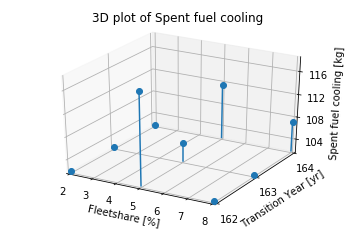
\includegraphics[width=0.4\linewidth]{figures/3d_sfc} 
        \caption{Inventory: Spent fuel cooling}
        \label{fig:3d_sfc}
    \end{subfigure}
    \begin{subfigure}[t]{0.4\textwidth}
        \centering
        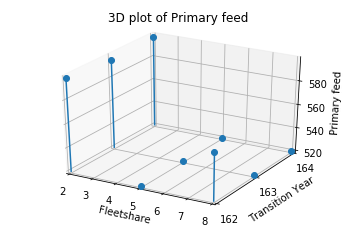
\includegraphics[width=\linewidth]{figures/3d_pf} 
        \caption{Inventory: Primary feed}
	    \label{fig:3d_pf}
    \end{subfigure}
    \begin{subfigure}[t]{0.4\textwidth}
        \centering
        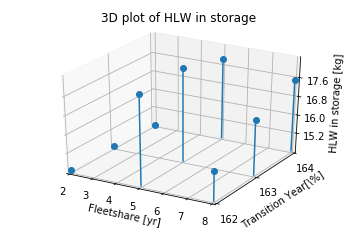
\includegraphics[width=\linewidth]{figures/3d_hlw} 
        \caption{Inventory: HLW in storage}
        \label{fig:3d_hlw}
    \end{subfigure}
    \caption{DYMOND EG01-30 Transition Scenario: ›Maximum amount of Pu [kg] in each inventory during each simulation for varying fleet share and transition start date.}
\end{figure}

Figures \ref{fig:3d_sfc}, \ref{fig:3d_pf}, and \ref{fig:3d_hlw}
communicate how fleet share ratio and introduction date of advanced 
reactor technology 
synergistically impact maximum Pu in various inventories in the 
\gls{NFC}. 
Similar synergistic studies can be conducted for the output variables in 
all the evaluation metrics to better utilize this information for decision making. 
The results from each study can be normalized, weighted, and 
combined to create an optimization surface similar 
to Figure \ref{fig:passerini_payoff} to determine the ideal fleet share 
ratio and transition year combination. 

\subsubsection{\textbf{Cyclus}}
We evaluated 25 scenarios for a combination of fleet share percentage 
of 0\%, 5\%, 10\%, 15\%, 20\% PWR MOX, and advanced reactor introduction 
date of year 80 to 84.
Figures \ref{fig:cyclus_3d_hlw}, \ref{fig:cyclus_3d_depu}, and 
\ref{fig:cyclus_3d_ic}
visualize the final amount of HLW, the final amount of depleted uranium, 
and the total amount of idle capacity in the scenario for varying 
fleet share and advanced reactor introduction date values. 

Figure \ref{fig:cyclus_3d_hlw} shows that for scenarios in which 
there is a smaller fleet share of \gls{MOX} \glspl{PWR}, and the 
transition begins later in the simulation, less high 
level waste produced. 
For a later transition year, we assume that the initial 
\glspl{LWR} have a longer lifetime
and thus, advanced reactors exist in the simulation for a shorter 
amount of time, resulting in a smaller production of reprocessing 
HLW waste. 
Also, \gls{MOX} \glspl{PWR} produce more \gls{HLW} than \glspl{SFR}. 
Figure \ref{fig:cyclus_3d_depu} shows that as the introduction date 
of advanced reactors is pushed back, more depleted uranium is produced 
due to the extended lifetime of the \glspl{LWR} that utilize enriched 
natural uranium fuel that generates depleted uranium. 
Figure \ref{fig:cyclus_3d_ic} shows that idle capacity is minimized 
for a later advanced reactor introduction date. 
Having a later introduction date of advanced reactor technology ensures 
that a sufficiently large inventory of transuranic elements is amassed
to produce fuel for the \gls{MOX} \glspl{PWR} and \glspl{SFR}.  
This ensures that there is no gap in the supply chain that results 
in idle advanced reactor capacity.

% replace transition year 
\begin{figure}[]
    \centering
    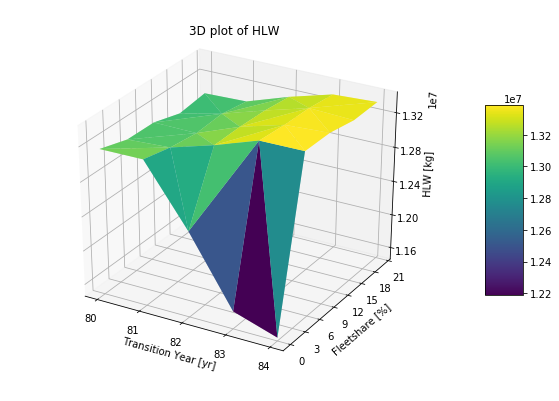
\includegraphics[width=0.7\linewidth]{cyclus_3d_hlw} 
    \caption{\Cyclus Transition Scenario: Final amount of HLW [kg] in the scenario during each simulation for varying fleet share and transition start date.}
    \label{fig:cyclus_3d_hlw}
\end{figure}

% replace transition year 
\begin{figure}[]
    \centering
    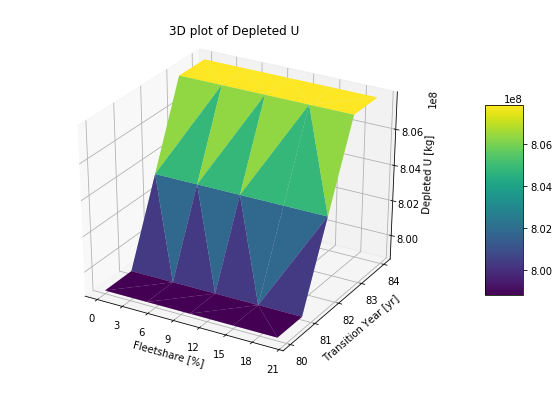
\includegraphics[width=0.7\linewidth]{cyclus_3d_depu} 
    \caption{\Cyclus Transition Scenario: Final amount of Depleted Uranium [kg] in the scenario during each simulation for varying fleet share and transition start date.}
    \label{fig:cyclus_3d_depu}
\end{figure}

% replace transition year 
\begin{figure}[]
    \centering
    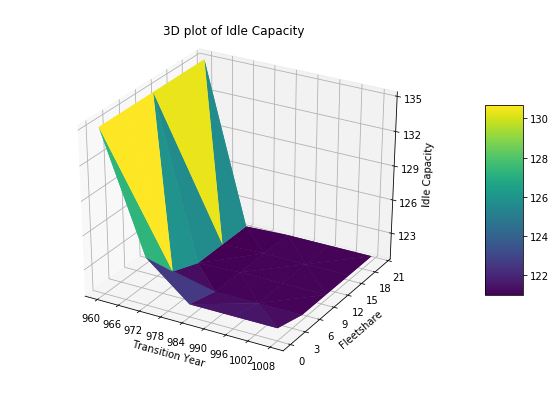
\includegraphics[width=0.7\linewidth]{cyclus_3d_ic} 
    \caption{\Cyclus Transition Scenario: Total amount of Idle Capacity [MW] in the scenario during each simulation for varying fleet share and transition start date.}
    \label{fig:cyclus_3d_ic}
\end{figure}

\section{Global Sensitivity Analysis}
\texttt{dcwrapper} was used to conduct a global sensitivity 
analysis study to generate Sobol indices, which tells us which 
input parameters have the most influence on an output variable.
Section \ref{sec:sobol} describes this type of sensitivity 
analysis.
It provides a more holistic view of the system 
than OAT (section \ref{sec:oat}) and 
synergistic (section \ref{sec:synergistic}) sensitivity 
analysis because it decomposes the variance of the 
output of the scenario simulation into fractions which can be 
attributed to each input, giving a better idea of the
most impactful input parameters. 
We could vary more than two variables in a synergistic 
sensitivity analysis, but it is difficult to visualize the results.

The input variables varied are fleet share ratio, 
transition start year, and used fuel cooling time.
The output variables considered are the final amount of HLW, 
the final amount of depleted uranium, and total idle capacity. 
Table \ref{tab:sobol} provides the Sobol indices that depict 
the impact of the variance of each input variable on each output 
variable. 
It provides a summary of the most influential input parameters 
for each output parameter. 
The Sobol indices are only comparable for each output variable 
(within each column). 
The fleet share has the largest impact on 
final HLW value, while the transition start year has the largest 
impact on final depleted uranium value and the total idle 
capacity value in the simulation. 
Transition start year and cooling time have some influence on 
the final value of HLW. 
Fleet share and cooling time do not influence the final 
depleted uranium value. 
    
    \begin{table}[H]
        \centering
        \doublespacing
        \caption{Sobol Indices for a global sensitivity analysis study of the impact of 
        fleet share \% of PWR MOX reactors, transition start year and cooling time on various output
        variables: final amount of HLW, final amount of depleted uranium, and total 
        idle capacity in the simulation. The Sobol Indices are only comparable within each column, 
        not within each row.}
        \label{tab:sobol}
            \small
            \begin{tabular}{l|lll}
                \hline	
                \multicolumn{4}{c}{\textbf{Sobol Indices for Output Variables}}   \\ \hline
                \textbf{Input Variables} & \textbf{Final HLW} & \textbf{Final depleted uranium} & \textbf{Total idle capacity} \\ \hline
                \textbf{Fleet Share} & 0.828     & 0                      & 0.00509             \\
                \textbf{Transition Year}                & 0.381     & 0.971                  & 1.505               \\
                \textbf{Cooling Time}                         & 0.126     & 0                      & 0                   \\ \hline

            \end{tabular}
    \end{table}

These global sensitivity analysis results give a good idea of the influence each 
input variable has on the output variables of interest. 
From Table \ref{tab:sobol}, we can inform the types of synergistic and one-at-a-time 
sensitivity analysis that should be done 
to understand the transition scenario system better. 
To better understand the impact of these three input parameters on final depleted 
uranium and total idle capacity, a one-at-a-time sensitivity analysis of transition 
year is sufficient. 
To better understand the impact of these three input parameters on the final HLW 
amount, a synergistic sensitivity analysis of share and cooling time is required.

\section{Main Takeaways}
\subsection{DYMOND Limitations}
For a transition scenario simulation in DYMOND, the user must 
manually edit the fuel management 
strategy to define which reactor the recycled 
part of each fuel type comes from for every year. 
Having the wrong fuel management strategy results in idle reactor
capacity due to the lack of fuel. 
Therefore, the user has to use trial and error to find a fuel 
management strategy to minimize or eliminate idle reactor capacity. 
With a 300-year simulation taking a few hours to run, it quickly 
becomes very tedious and time-consuming.  

This issue impacts sensitivity analysis conducted 
with DYMOND because the fuel management strategy was 
optimized manually for specificß scenario parameters, resulting in 
idle reactor capacity occurring when scenario parameters differed 
from it. 
An AI-based method (similar to \deploy) 
should be introduced to 
determine where the recycled part of each fuel comes from to 
minimize idle capacity in the simulation. 
This eases the setting up of transition scenarios, and enable 
more effective and accurate sensitivity analysis studies.

\subsection{Importance of Different Types of Sensitivity Analysis}
The OAT, synergistic, and global sensitivity analysis methods 
are all key to analyzing \gls{NFC} transition scenarios. 
In this chapter, we demonstrated each sensitivity analysis type. 
Each method has its advantage. 
When conducting a comprehensive sensitivity analysis of a specific 
transition scenario, 
global sensitivity analysis should be conducted first to 
determine which input variables are key to influencing the output 
variables of interest. 
OAT and synergistic sensitivity analysis can then be used together to 
do further analysis to determine the trends and quantitative impacts 
of specific input variables on specific output variables. 
Synergistic sensitivity analysis is useful for analyzing 
tightly coupled input variables.  

\chapter{Conclusion}

% difference between cyclus and dymond 
% cyclus is more flexible but harder to use 
% dymond is rigid in the type of scenarios to run 
% more comparisons of cyclus and dymond in this section 
%or after demonstration. 

\Cyclus is shown to be flexible in setting up successful transition 
scenarios when input parameters are slightly varied.
DYMOND is able to successfully set up a transition scenario, if the 
user ensures to set up a fuel management strategy correctly. 
It is important that \glspl{NFCSim} are flexible and resilient to 
perturbations in transition scenario input parameters. 
Despite 

% for sensitivity analysis 

%%%%%%%%%%%%%%%%%%%%%%%%%%%%%%%%%%%%%%%%%%%%%%%%%%%%%%%%%%%%%%%%%%%%%%%%%%%%%%%
% APPENDIX
%
%\appendix
%\include{apx}

\backmatter

%%%%%%%%%%%%%%%%%%%%%%%%%%%%%%%%%%%%%%%%%%%%%%%%%%%%%%%%%%%%%%%%%%%%%%%%%%%%%%%
% BIBLIOGRAPHY
%
%\bibliographystyle{IEEE_ECE}
\bibliographystyle{unsrt}
% Put references in BibTeX format in thesisrefs.bib.
\bibliography{thesisrefs}

\end{document}
\endinput
